% ============================================================
% Intervention-aware tests of useful emergence
% Target: Nature Machine Intelligence (single-column draft)
% Every number in this file is backed by a script + output file
% in the repository (see Methods and REPRODUCIBILITY.md).
% ============================================================
\documentclass[11pt]{article}

\usepackage[a4paper,margin=2.5cm]{geometry}
\usepackage{amsmath,amssymb,amsthm}
\usepackage{graphicx}
\usepackage{booktabs}
\usepackage{array}
\usepackage{multirow}
\usepackage{xcolor}
\usepackage[font=small,labelfont=bf]{caption}
\usepackage{microtype}
\usepackage[colorlinks=true,linkcolor=blue!60!black,citecolor=blue!60!black,urlcolor=blue!60!black]{hyperref}

\graphicspath{{./}{../figures/}}

\newtheorem{proposition}{Proposition}
\setcounter{proposition}{-1}   % Proposition 0 is the root definition
\newtheorem{corollary}{Corollary}
\theoremstyle{definition}
\newtheorem{definition}{Definition}

\newcommand{\dO}[1]{\mathrm{do}(#1)}
\newcommand{\KL}{\mathrm{KL}}
\newcommand{\JS}{\mathrm{JS}}
\newcommand{\TV}{\mathrm{TV}}
\newcommand{\EI}{\mathrm{EI}}
\newcommand{\CE}{\mathrm{CE}}
\newcommand{\Ptb}{P_t(B \mid s_t)}

\title{\textbf{Useful possibility collapse identifies adaptive\\emergent structure in learning systems}}
\author{[Authors]\\[2pt]\small [Affiliations]}
\date{}

\begin{document}
\maketitle

% ============================================================
\begin{abstract}
\noindent
Emergence is used to describe abrupt abilities, collective coordination,
representational phase changes, synergy and macro-causal efficacy, yet
these signatures often disagree. We propose an intervention-aware
framework that identifies \emph{adaptive emergence} in learning systems
as \emph{useful possibility collapse}: the endogenous formation and
stabilization of a valuable macro-structure in an open conditional
future distribution. A known trajectory-space substrate fixes what is
measured; the output is a six-component certificate plus a calibrated
continuous record whose dimensions demonstrably measure the constructs
they name against a ground-truth generator. The same frozen thresholds
identify learned systems and reject scripted and initialization
controls in three built domains and---under an externally timestamped
preregistration---in the public Overcooked-AI benchmark, where all
five registered predictions passed. Multivariate combinations of prior
measures with equal freedom fail to transfer to fresh systems, and a
future-distribution score prospectively discovers value-critical
decisions in uncurated human chess. Emergence becomes testable rather
than curve-read.
\end{abstract}

\vspace{1em}

% ============================================================
``Emergence'' may be the most load-bearing and least agreed-upon word
in the science of complex and learning
systems~\cite{anderson1972,bedau1997,holland1998,mitchell2009,crutchfield1994,batterman2002}.
Four communities measure it four ways: abrupt performance curves in
large language
models~\cite{kaplan2020,brown2020,bommasani2021,hoffmann2022,wei2022,ganguli2022,srivastava2023},
sudden representation jumps, informational
synergy~\cite{williamsbeer2010,bertschinger2014,lizier2018,rosas2020,mediano2021,luppi2022},
and macro-level causal efficacy under
intervention~\cite{hoel2013,hoel2025,barnett2023}.

These are not four estimators of one agreed-upon quantity but distinct
operational definitions that yield conflicting verdicts: Wei et
al.~\cite{wei2022} call LLM abilities emergent; Schaeffer et
al.~\cite{schaeffer2023} show the same curves can be artifacts of the
metric and sampling grid, and no performance curve carries information
about where an ability came from. Synergy and causal-emergence
measures quantify macro-structure without encoding whether it was
selected by the system, useful in context, or acquired rather than
imposed. Here we organize these signatures on systems with an explicit
trajectory law and value structure: each audited quantity is a
deterministic functional of the same trajectory-law family
(Proposition~\ref{prop:coverage}), yet none of them---alone
(Proposition~\ref{prop:nosingle}), in exact published form on fully
enumerated chains, or in fitted multivariate combination---reproduces
the predeclared labels on a controlled battery, because no projection
retains the value sign, the conditional selectivity, and the
provenance of the collapse together.

What, then, do we propose to measure? The claim is deliberately scoped:
we do not offer an observer-free definition of all emergence in nature,
but an identification framework for \emph{adaptive emergence acquired
during learning}. Its layers are explicit. A system holds an \emph{open
possibility space}---many future basins with non-trivial probability;
an \emph{endogenous trigger}---an action or learning event chosen by
the system, often locally costly---collapses that distribution
\emph{selectively} (conditioned on context) and \emph{specifically}
(triggered futures differ from non-triggered ones). This much is
\emph{structural collapse}, and it can occur in harmful or prewired
systems. The event qualifies as adaptive emergence only when the
collapse is also \emph{useful} (a positive value do-contrast, assessed
through model-based interventions~\cite{pearl2009}), \emph{endogenous}
and \emph{acquired} rather than prewired. In one sentence:
\emph{adaptive emergence is the stabilized, useful collapse of an
acquired behavioural structure in an open possibility space}. Six
components---potential, selectivity, specificity, usefulness,
endogeneity, acquisition---make this falsifiable; thresholds were
frozen before the confirmatory measurements to which they applied. The
layering preserves what a single conjunction would flatten: harmful
collapse and scripted coordination are structurally emergent but not
adaptive, and both cases are measured systems in our batteries rather
than rhetorical categories.

The mathematical starting point is honest about its lineage. The
trajectory-space object we use is a standard specific-information
quantity, the same posterior--prior divergence that defines Bayesian
surprise~\cite{ittibaldi2009,deweese1999}; related future-facing
quantities---empowerment as an action--future channel
capacity~\cite{klyubin2005,salge2014}, causal path-entropy
forces~\cite{wissnergross2013}, and semantic information as
viability-relevant syntactic information~\cite{kolchinsky2018}---have
long used information and intervention to separate valuable from
incidental structure. What these frameworks do not supply, and what
this paper adds, is an identification protocol for \emph{when} a
selective, valuable, acquired contraction of the future distribution
should count as emergence: the substrate is known mathematics; the
contribution is the layered criterion, its falsification battery, and
its cross-domain transfer under frozen thresholds.

The paper then does four things. \emph{First}, it shows why the prior
signatures conflict: on a controlled battery each is a lossy
projection of one trajectory-law family, and named imitations fail
exactly the components they are built to fail---neither single prior
signals nor their fitted multivariate combinations transfer to fresh
systems. \emph{Second}, it fixes what is reported: the primary output
is a multi-dimensional record (certificate, causal magnitude, signed
value, abruptness, acquisition, persistence, uncertainty), with scalar
summaries declared secondary; the record's dimensions are calibrated
against a ground-truth generator and satisfy eight machine-verified
axioms. \emph{Third}, it validates: the full six-component conjunction
confirms under frozen thresholds in three built system families---an
external swarm, Contextual Level-Based Foraging, and a latent-context
sequence model---and, under an externally timestamped preregistration,
in the public Overcooked-AI benchmark. \emph{Fourth}, it shows what
the account buys beyond postdiction: a derived phase boundary
forecasts where emergence appears in a parametrized family before
training; an event-level score performs prospective discovery in
uncurated chess play; and the process proxy recovers
grokking~\cite{power2022,nanda2023} and induction-head
formation~\cite{olsson2022,elhage2021} and selected transitions in
public MultiBERTs~\cite{sellam2022} and Pythia~\cite{biderman2023}
series while rejecting gradual controls. Registered failures are
retained and delimit scope, including the martingale lesson that
converged policies price their own triggers into the baseline, so
useful collapse in that regime is visible only through do-contrasts.

% ============================================================
\section{Results}

\subsection*{A trajectory-space framework for emergence}
\label{sec:framework}


\textbf{The substrate: a known information quantity.}
Let $\tau$ be a system trajectory with prior law $P(\tau)$---the open
possibility space---and let $M$ record which basin, ability or outcome
materialized. The trajectory-space information associated with observing
structure $m$ is
\begin{equation}
  C(m) \;=\; \KL\!\bigl( P(\tau \mid M{=}m) \,\big\|\, P(\tau) \bigr)
  \qquad [\text{bits}].
  \label{eq:root}
\end{equation}
Equation~\eqref{eq:root} is not new mathematics and is not, by itself, a
definition of emergence: it is the specific-information form of Bayesian
surprise~\cite{ittibaldi2009,deweese1999}, and it depends only on how
rare the realized macro-outcome is ($\mathbb{E}_{m}C(m)=I(\tau;M)$; for
deterministic readouts $C(m)=-\log_2 P(A_m)$). Its role here is to fix
the \emph{space} on which emergence claims must live---distributions
over futures, not points in representation space or scores on a
metric. Three statistics that the word ``collapse'' could conflate are
connected by an exact bridge:

\begin{proposition}[Collapse bridge]\label{prop:bridge}
At a declared step with action distribution $\pi$ and a fixed rollout
law thereafter (so that choosing $a$ and $\dO{a}$ induce the same
future law), the action-attributable prospective contraction
$H(P_t(B)) - \mathbb{E}_{a\sim\pi} H(P(B \mid \dO{a}))$, the
$\pi$-averaged interventional divergence
$\mathbb{E}_{a\sim\pi} \KL(P(B \mid \dO{a}) \,\|\, P_t(B))$, and the
expected retrospective update
$\mathbb{E}_{b} \KL(\pi(A \mid B{=}b) \,\|\, \pi(A))$ all equal
$I(A;B)$. A deterministic policy has $I(A;B)=0$.
\end{proposition}

The bridge separates system-driven collapse from ordinary information
revelation: every resolving stochastic process concentrates its
posterior, but only the contraction attributable to the system's own
action choice is common to all three readings, and it vanishes for
deterministic controllers---which is why greedy decisions carry no
potential, and why all measurements below use the prospective,
interventional forms (identities verified to machine precision on
10,000 random systems and on trained trigger steps; Methods).

The substrate also shows why it cannot carry the verdict alone: on the
fully enumerated battery chains, raw path-space KL is large in controls
too (converged team $32.2$ bits, shaped process $31.9$ bits), and only
the declared value-bearing basin projection separates the accepted
system ($32\%$ of its trajectory-level contrast retained, against
$3\%$ and $0.01\%$ for controls). The discriminating content lives in
the observer contract---a basin partition $B=g(\tau)$ that resolves the
candidate macro-structure, a value function, a rollout policy,
interventions and a time resolution---and in the component criteria
built on it. This is the architecture of the framework, not a
limitation discovered after the fact: known substrate, declared
contract, layered criteria.

\textbf{Layered identification criteria.}
A collapse event is scored under a declared observer contract in two
layers:
\begin{definition}[Structural collapse]
\label{def:structural}
An episode-level event is a structural collapse iff it has
(1)~\textbf{Potential}, an open future before the event;
(2)~\textbf{Selectivity}, context-dependent rather than unconditional
collapse; and
(3)~\textbf{Specificity}, triggered futures that differ from
non-triggered futures.
\end{definition}
\begin{definition}[Adaptive emergence]
\label{def:criterion}
A structural collapse qualifies as adaptive emergence iff it also has
(4)~\textbf{Usefulness}, a positive value do-contrast;
(5)~\textbf{Endogeneity}, a trigger chosen by the system rather than
imposed; and (6)~\textbf{Acquisition}, a gain over the system's own
initialization.
\end{definition}
The two layers are not decoration: harmful collapse (a decoy trap) and
scripted coordination are structural collapses that fail the adaptive
layer, and both are measured systems below. The layering also predicts
an asymmetry that we test directly: structural components are
properties of the future distribution and should survive a change of
observer contract that still resolves the macro-structure, whereas
usefulness is value-relative \emph{by declaration} and may not.

Where six components are unavailable, we use scoped instruments
instead: chess is an event-level test without acquisition,
non-contextual deep MARL is a mechanism-level do-contrast test, and
checkpoint series use a separate four-component process proxy in which
burstiness measures acquisition velocity, not emergence magnitude
(Table~\ref{tab:scope-map}). The six components are identification
criteria motivated by the substrate and validated by falsification
below; they are not claimed to be uniquely derivable from
Eq.~\eqref{eq:root}.

The exclusions are empirical, not stipulated: deterministic greedy
controllers have no open future; gradual frequency learning fails the
burst component of the process proxy; scripted, forced and prewired
systems fail provenance; memorization and harmful traps collapse
possibilities without useful do-contrast. The verdict is a
\emph{conjunction} for a measured reason: a large factor would
otherwise buy back a deficient one. Thresholds and analysis windows
were frozen in code and per-domain author-maintained protocols before
each confirmatory measurement; throughout, ``registered'' means
\emph{internally frozen} in these hash-anchored records---no protocol
was third-party registered and no external timestamp is claimed,
with one exception: the Overcooked-AI confirmation protocol carries a
public timestamp that predates every confirmatory measurement
(Methods).

Figure~\ref{fig:concept} gives the conceptual picture: four regimes of
$\Ptb$ that performance or representation jumps conflate---forced
convergence (the future was never open), structureless openness (open
but never collapses), harmful collapse (a structural collapse that
fails the adaptive layer), and useful possibility collapse. Only the
last is adaptive emergence under Definition~\ref{def:criterion}, and
each of the other three is a measured system in our battery, not a
hypothetical.

\begin{figure}[t]
  \centering
  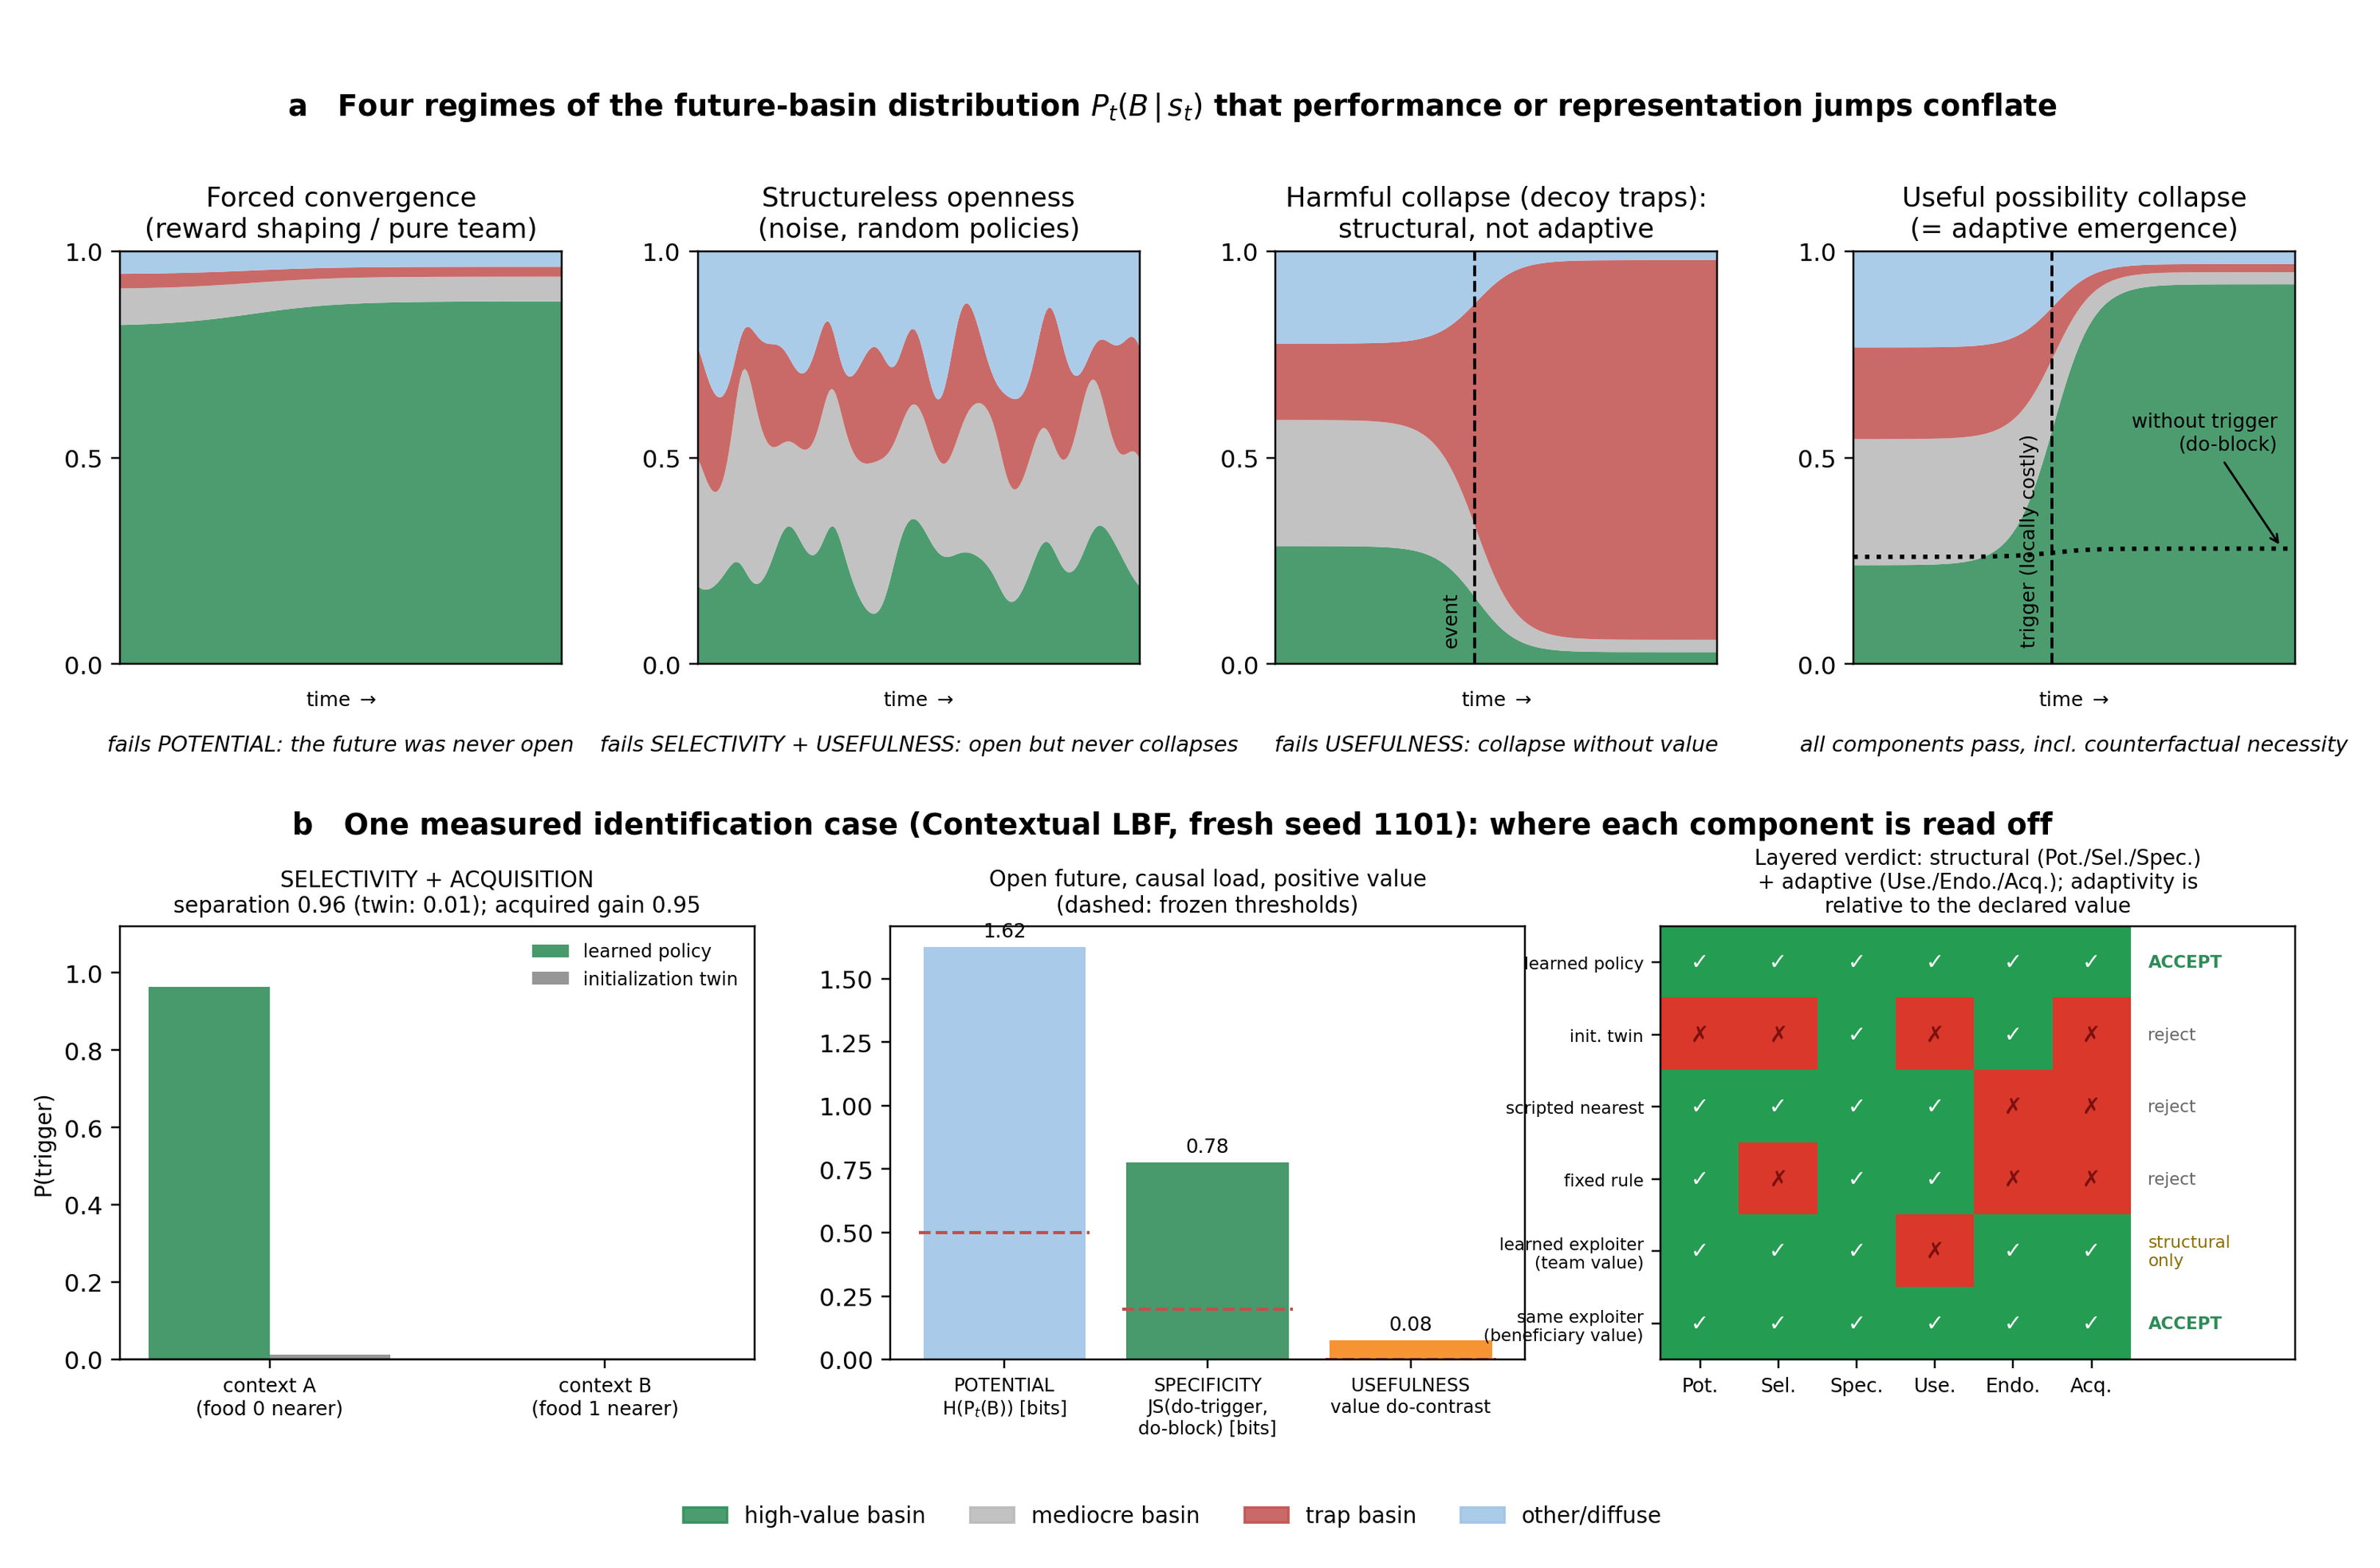
\includegraphics[width=\linewidth]{main_fig1.png}
  \caption{\textbf{Four regimes of the future-basin distribution, and
  one measured identification case.}
  \textbf{a}, The observer's future-basin distribution $\Ptb$
  separates regimes that performance or representation jumps conflate:
  forced convergence fails Potential; structureless openness fails
  Selectivity and Usefulness; harmful collapse is structural but not
  adaptive (fails Usefulness); useful possibility collapse passes all
  components, and the do-blocked counterfactual (dotted) shows the
  future would otherwise have stayed open.
  \textbf{b}, Where each component is read off, on one stored
  Contextual LBF case (fresh seed 1101): per-context trigger rates
  against the initialization twin give selectivity ($0.96$ vs $0.01$)
  and acquisition ($+0.95$); potential, do-contrast specificity and
  the value do-contrast clear their frozen thresholds (dashed); and
  the layered checklist accepts the learned policy while rejecting the
  twin, a competent scripted controller (fails exactly the adaptive
  layer) and a fixed rule.}
  \label{fig:concept}
\end{figure}

\subsection*{Prior signatures diverge on a controlled battery}
\label{sec:battery}

\begin{proposition}[Single-observable insufficiency on the audited battery]\label{prop:nosingle}
For each tested scalar observable
$O \in \{$potential $H(P_0)$; collapse burst; specificity JS;
usefulness gap; representation jump; causal-emergence EI$\}$, no
one-sided threshold reproduces all predeclared labels on the measured
battery. The best hindsight-selected threshold accuracies are
$0.800$--$0.900$.
\end{proposition}

The result follows by exhaustive threshold sweep, with measured
witnesses in Methods (Table~\ref{tab:witnesses}). Representation
distance illustrates all three failure modes at once: the harmful
decoy has the \emph{same} jump ($0.102$) as the true conditional
emergence (usefulness $+3.43$ vs $-8.39$; a norm carries no sign), the
genuine case jumps \emph{less} than reward-shaped ($0.403$) and
converged-team ($0.328$) controls, and a noisy learner with the same
selective structure jumps $13.7\times$ farther. Collapse upper-bounds
the jump (Proposition~\ref{prop:pinsker}): a jump certifies that the
distribution moved, never where it landed nor who moved it.

On the designed battery the component conjunction scores $1.000$
against predeclared labels (Fig.~\ref{fig:battery}a); after one
registered selectivity failure and a disclosed refinement, the frozen
rule confirms on a fresh internal seed (10/10) and on 25/25 fresh
external swarm verdicts with measured acquisition (Methods). Dropping
selectivity, usefulness or endogeneity re-admits its named
counterexample; every single prior observable, even at its
hindsight-optimal threshold, caps at $0.800$--$0.900$
(Fig.~\ref{fig:battery}a,b).

\textbf{Exact rival formalisms within declared candidate families.}
Because charitable proxies could misrepresent the rival definitions, we
also computed Hoel's EI/CE and Rosas' $\Psi$ exactly, with zero
Monte-Carlo error, on fully enumerated policy-closed Markov chains of
all ten systems (up to $75{,}004$ states)---exact evaluations
\emph{within predeclared restricted candidate families}, not
exhaustive searches over all coarse-grainings or features. Exact CE
(over a five-member coarse-graining family containing the
mechanistically privileged partitions) is negative for every system;
its best threshold is the trivial all-negative classifier (accuracy
$0.8$, missing both positives). Exact $\Psi$ (maximized over four
supervenient features and two micro decompositions) scores $0.3$ under
its published sign rule, its top scorer is the wrong-selector system
($+0.59$), and its hindsight optimum requires inverting the published
sign convention while still missing the true conditional emergence
(Fig.~\ref{fig:battery}c). The blind spots---no access to value sign,
natural selectivity, or provenance---are structural on this testbed.

\textbf{A graded measurement from the rarity identity.}
The substrate also predicts a gradient no audited signature supplies:
the less the training signal biases search toward a macro-structure,
the rarer that structure is under the provenance's early search
distribution ($C=-\log_2 P$). Measured for one macro-pattern under
three provenances, the seed-mean ordering is as predicted---scripted
$0$ $<$ process-shaped $0.39$ $<$ outcome-only $0.65$ bits, with
discovery twice as late at matched final competence---while outcome
rarity and structural magnitude are provenance-indistinguishable by
construction, so the three quantities a single ``strength'' number
would conflate are reported separately. The registered suddenness
ordering failed and is retained: both acquisitions are step-like, so
this is a provenance-adjusted discovery surprise, not a universal
magnitude (Extended Data Fig.~\ref{fig:ed-strength}).

\textbf{Harmful emergence and matched provenance.}
Two constructions make the layering load-bearing (nine registered
predictions, all passed). A policy trained on an exploiter reward
\emph{learns} a harmful structure on 5/5 seeds: it selectively lures
its partner onto the decoy in exactly the harmful context, passes
every structural component, and its value do-contrast is $+7.5$ under
the declared beneficiary's value while $-2.0$ under the team
value---structurally emergent under both values, adaptive only for its
beneficiary. And four systems with matched natural behaviour (script,
behavioural clone, shaped and outcome-only learners; pattern
probability $\ge0.99$ for all) separate what a provenance flag alone
could not: the do-contrast distinguishes the clone from its source
(specificity $0.38$--$0.45$ vs $1.0$ bits---forcing the clone off its
training distribution exposes states it never memorized); acquisition
separates static from trained provenance; and provenance rarity orders
the trained routes (clone $0.33$ $<$ shaped $0.39$ $<$ outcome-only
$0.65$ bits).

\textbf{A continuous record under the certificate.}
The binary certificate prevents dimensional compensation; a continuous
record answers \emph{how strongly, how abruptly and in which
direction}. Each system receives a declared vector---normalized
potential, selectivity, causal magnitude, signed value, acquisition,
abruptness---whose aggregation was fixed before calibration and never
fitted to labels. That these dimensions are measured constructs rather
than plausible design is established against ground truth: a
six-knob generator whose parameters independently control each
construct by construction, measured through the same finite-sample
estimator pipeline as the real systems, yields a diagonally dominant
sensitivity matrix with no violation (Extended Data
Fig.~\ref{fig:ed-generator}); the value knob spans $1.52$ of $V$ while
moving $M$ by less than $0.001$, and the acquisition knob spans $0.99$
of $Q$ at unchanged structure. Nullity, value separability, provenance
separability and dose--response monotonicity (Spearman $1.0$, 5/5
seeds) passed as registered; the off-diagonal suppression rule failed
on two couplings and is retained (one exemption-list specification
error; persistence responds to structure at $0.29$ of its diagonal
because retention is retention \emph{of} structure). Eight axioms of
the record are machine-verified, and observer freedom is itself a
computable quantity: across the stored admissible contracts, per-seed
structural scores carry identification intervals of median width
$0.14$ with a stable ranking (mean pairwise Spearman $0.76$), and no
control's interval touches the adaptive layer. The record's honest
boundary is predictive: three registered early-prediction rules failed
and are retained---structure-only scores cannot separate scripted from
learned (the layering's own claim, re-derived), and near phase
boundaries early causal magnitude does not beat early performance at
predicting acceptance, though each dimension does predict its
\emph{own} endpoint (early magnitude forecasts final structure at
Spearman $0.56$ where performance is uninformative at $-0.09$). The
predictive content is axis-specific, not a universal improvement over
performance.

\textbf{Multivariate prior-signal baselines with equal freedom.}
Comparing one scalar against a six-threshold conjunction would be
asymmetric, so we gave the prior signals equal or greater freedom and
tested generalization rather than fit. Hindsight AND-rules over pairs
or triples of prior signals, logistic regression and a depth-2 tree on
all signals (including exact EI and $\Psi$) reach $0.9$--$1.0$
in-sample, drop to $0.7$--$0.8$ under leave-one-out CV, and---frozen
and applied to a fresh-seed battery on which the frozen six-component
protocol had already scored $10/10$---transfer at $0.7$--$0.9$, with
every baseline misclassifying the true conditional emergence; our own
two-component AND-rules transfer no better ($0.7$--$0.8$). What the
projections lack is not fitting capacity but the selectivity, value
and provenance information they discard (Fig.~\ref{fig:battery}d).

\begin{figure}[t]
  \centering
  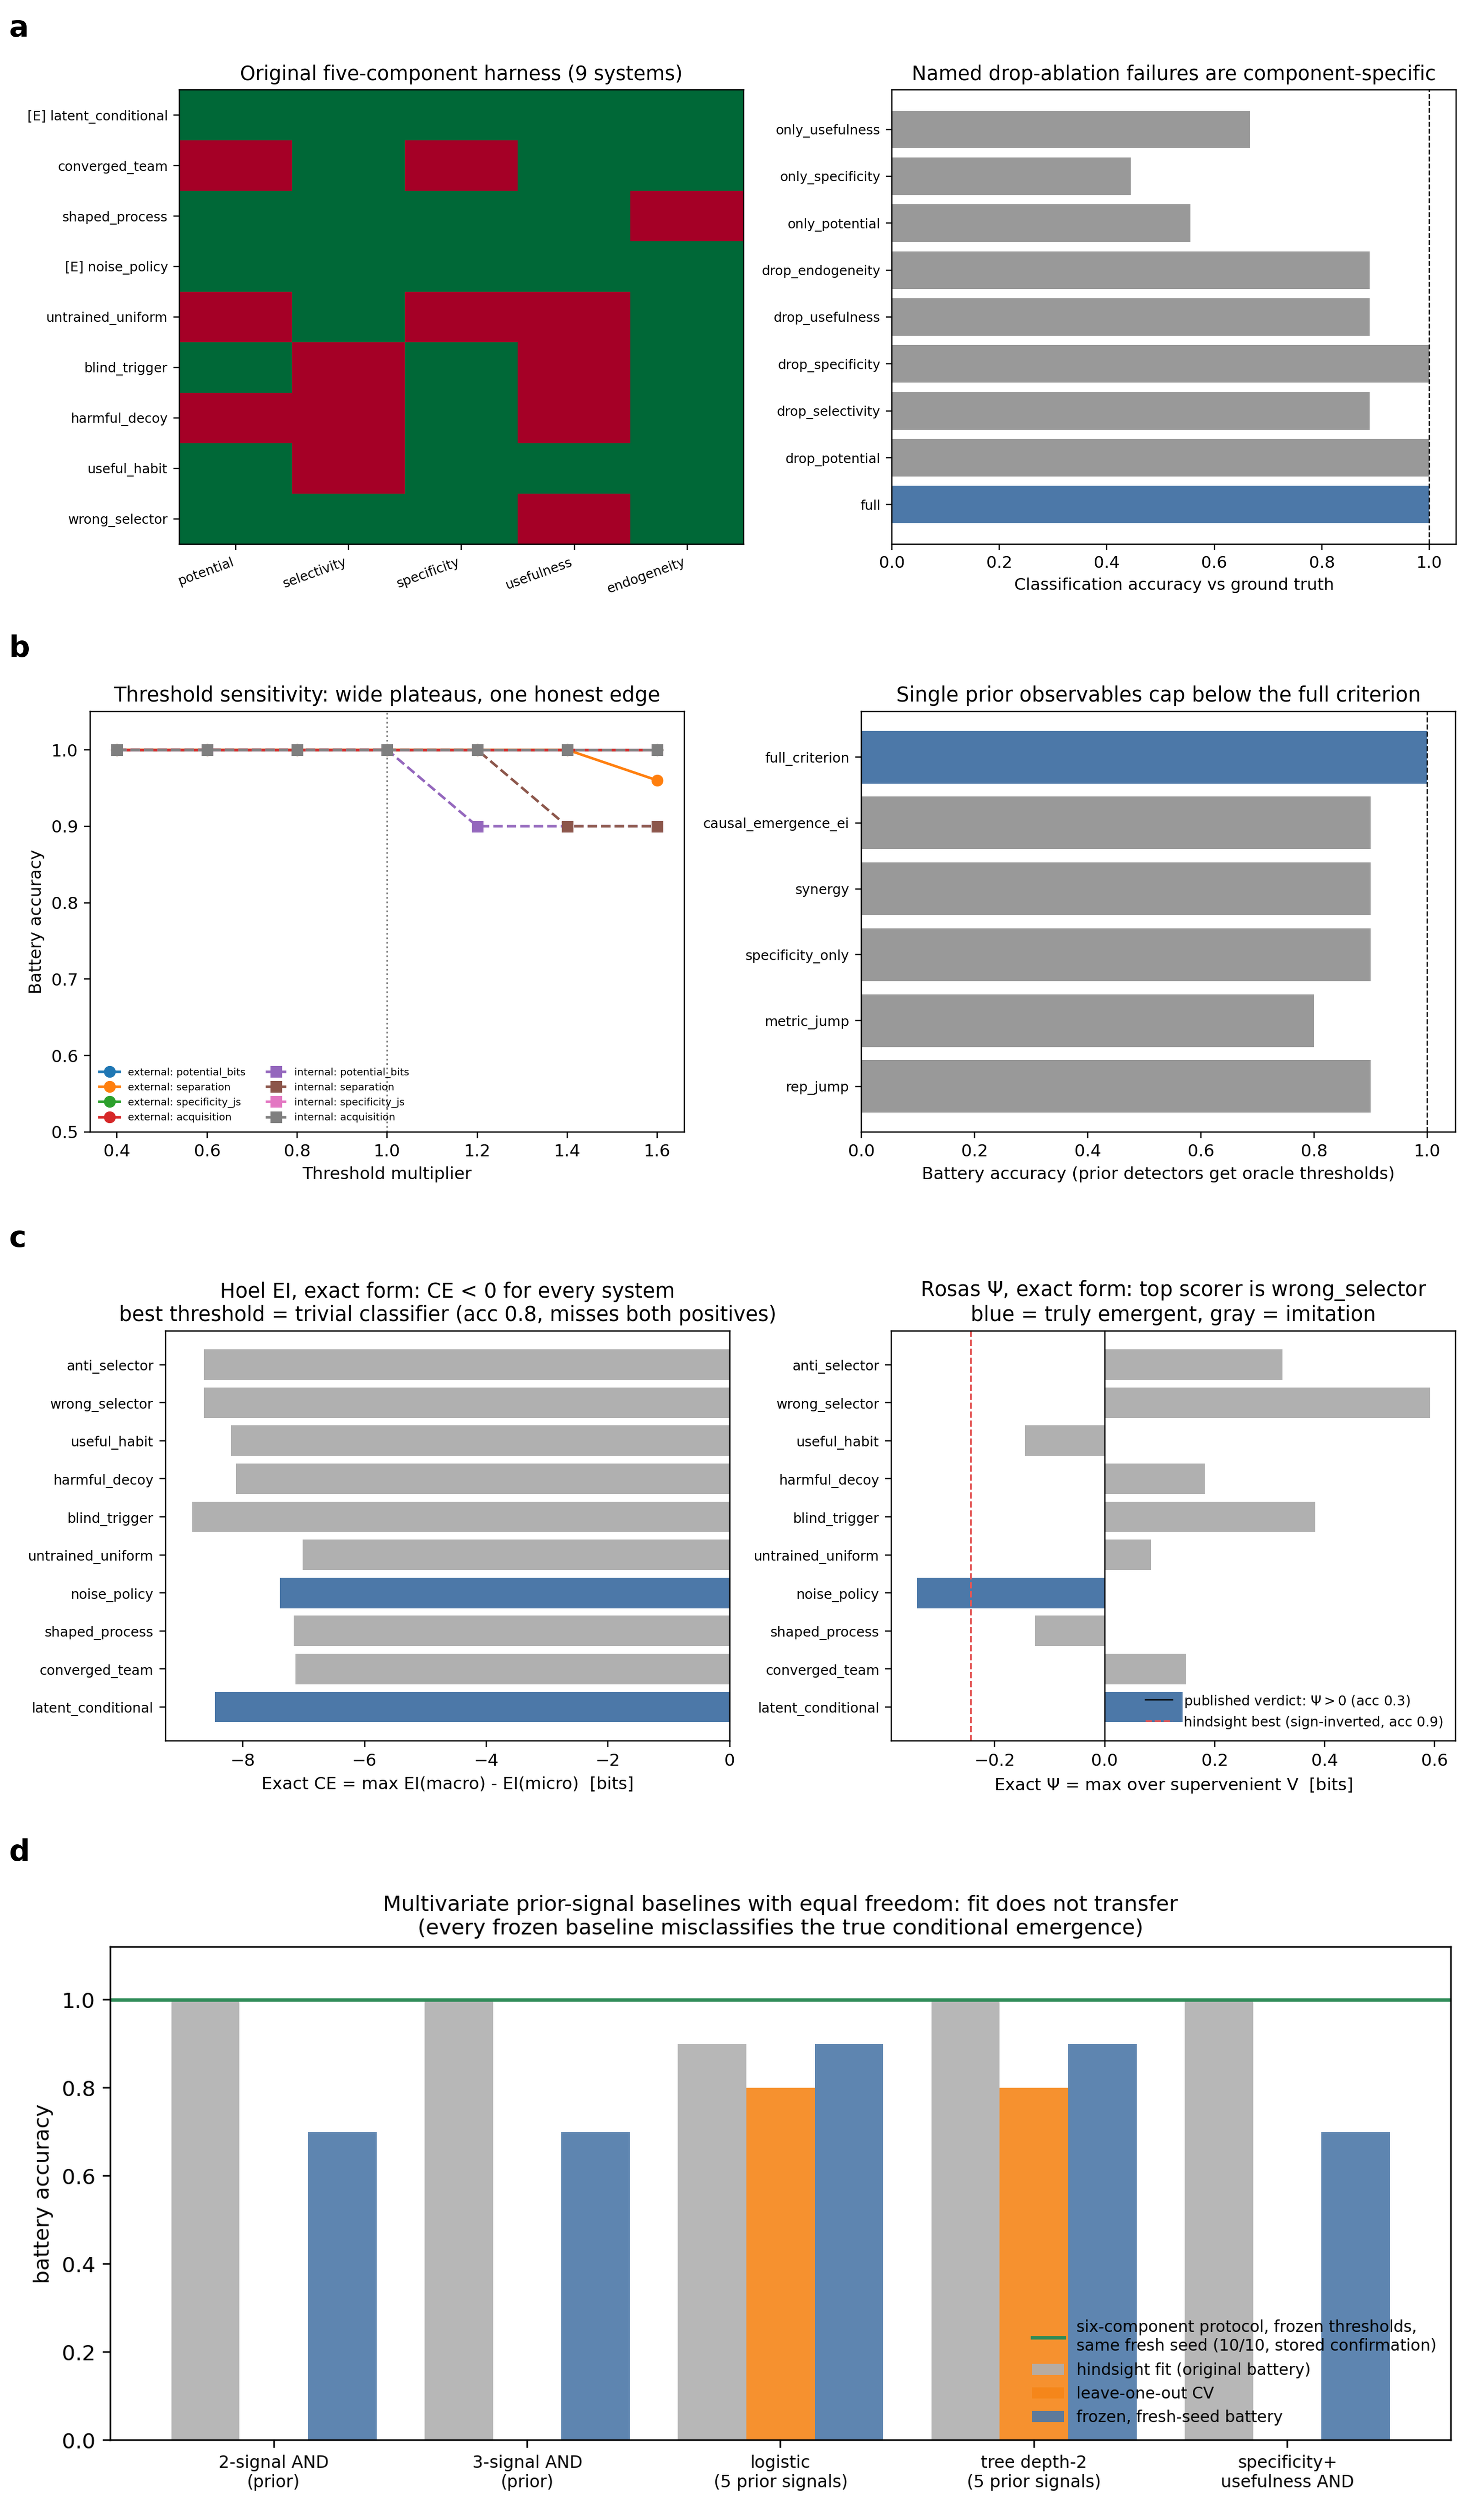
\includegraphics[width=\linewidth]{main_fig2.png}
  \caption{\textbf{The original conjunction separates predeclared positives from
  imitations on the shared battery; no tested single signature does,
  including published-form rival audits within declared candidate
  families.}
  \textbf{a}, Original internal component battery: component pass/fail
  per measured system (left); the original conjunction is exact on these
  predeclared labels, while
  dropping selectivity, usefulness or endogeneity admits its named
  counterexample and single-component rules fail (right).
  \textbf{b}, Registered thresholds sit on wide accuracy plateaus
  (left); single prior observables cap below the original conjunction even
  with hindsight-optimal (oracle) thresholds (right).
  \textbf{c}, Rival equations computed with zero Monte-Carlo
  error on enumerated chains: Hoel's exact CE is negative for every
  system and its best threshold is the trivial classifier, missing
  both true positives (left); Rosas' exact $\Psi > 0$ scores $0.3$
  with the wrong-selector as top scorer, and the hindsight optimum
  requires inverting the published sign convention (right). Blue =
  truly emergent systems; gray = imitations.
  \textbf{d}, Multivariate baselines with equal or greater freedom
  (per-signal thresholds and directions, logistic regression, depth-2
  tree, two-component AND rules) fit the original battery but drop
  under leave-one-out CV and, frozen, transfer at $0.7$--$0.9$ to a
  fresh-seed battery---every one missing the true conditional
  emergence---while the frozen six-component protocol scores 10/10 on
  the same fresh seed.}
  \label{fig:battery}
\end{figure}

\subsection*{Possibility collapse within single episodes}
\label{sec:mechanism}

The definition is about futures, so it is measured \emph{while the
future is still open}: within single episodes we estimate $\Ptb$ by
rollouts and apply do-operators at the trigger step (Extended Data
Fig.~\ref{fig:ed-mechanism}). The same action yields positive return
gaps in the rescue context and negative gaps in the bridge (decoy)
context---the directional content no unsigned jump carries. The basin
partition is not hand-picked: label-free clustering recovers the
designed basins with purity $1.00$ in all displayed regimes (one
registered partial failure on pure-team loss episodes is retained). A
neural replication reproduces the sign structure, and neural embedding
jumps track collapse bursts (correlation $0.87$--$0.90$, peak
alignment $1.0$)---the representation jump appearing exactly where
Proposition~\ref{prop:pinsker} says it must, as a downstream symptom.

\begin{proposition}[Collapse bounds representation jump]\label{prop:pinsker}
Let $R_t = \mathbb{E}_{B \sim P_t}[\phi(B)]$ for a feature map $\phi$,
$J_t = \lVert R_t - R_{t-1}\rVert_2$, and
$K_t = \KL(P_t \,\|\, P_{t-1})$ in bits. Then
\begin{equation}
  J_t \;\le\; \mathrm{diam}(\phi)\, \TV(P_t, P_{t-1})
      \;\le\; \mathrm{diam}(\phi) \sqrt{\tfrac{\ln 2}{2}\, K_t }.
  \label{eq:pinsker}
\end{equation}
\end{proposition}

Burst-like collapse \emph{can} produce representation jumps---which is
why jump-based observables fire when collapse happens---but the
converse fails: a large $J_t$ certifies only that the distribution
moved, not that the movement was a useful collapse. The bound was
verified numerically at every step of every trajectory in four
training regimes and both grokking conditions.

\begin{proposition}[Counterfactual necessity credits selectivity]\label{prop:usefulness}
Let a system trigger with probability $p_c$ in context $c$ (contexts
drawn with probability $w_c$), and let $V_c(a)$ be the expected return
under $a \in \{\text{trigger}, \text{non-trigger}\}$. With
$U = \mathbb{E}[\text{return} \mid \text{behavior}] -
\mathbb{E}[\text{return} \mid \dO{\text{non-trigger}}]$,
\begin{equation}
  U \;=\; \sum_c w_c\, p_c \bigl( V_c(\text{trigger}) - V_c(\text{non-trigger}) \bigr).
  \label{eq:usefulness}
\end{equation}
\end{proposition}

A selective system ($p_c \approx 1$ where the trigger helps, $\approx
0$ where it harms) receives the full positive terms and none of the
negative ones: $U$ measures exactly the value of the selection
structure. A blind system receives the sign of the \emph{marginal}
effect---which is why blind triggering can show positive $U$ in
environments where triggering helps on average, and why usefulness
alone cannot replace selectivity. Equation~\eqref{eq:usefulness},
applied with the closed-form $V_c$ of a parametrized environment, is
also what powers the within-family prospective parameter forecast of
Section~\ref{sec:marl}.

\subsection*{Process probes detect acquisition in public models}
\label{sec:public}


A definition of emergence in learning systems must also account for
acquisition over training. Here the event is a checkpoint transition rather
than a do-blockable action, so we use the separate process proxy from
Table~\ref{tab:scope-map}: potential before the window, a collapse burst in
the future-basin distribution, usefulness gain on a fixed evaluation
battery and controls that share either collapse or performance symptoms.
This proxy measures acquisition \emph{velocity}; it is not a stand-alone
emergence verdict.

The proxy first recovers two cases with independently studied
mechanisms (Extended Data Figs.~\ref{fig:ed-grokking},
\ref{fig:ed-induction}, \ref{fig:ed-public}). Grokking transitions in
three architecture families pass the frozen potential, burstiness and
usefulness thresholds, while the memorization phase in the same run is
rejected: held-out entropy collapses ($6.6\to2.8$ bits) with no
accuracy gain. The two-layer attention-only model that can implement
induction passes all components (copy accuracy $0.987$); the one-layer
architecture that cannot fails usefulness ($0.112$).

On public series the same protocol transfers as a resolution-limited
instrument. MultiBERTs subject--verb agreement collapses from a
$14.7$-bit masked-verb space in a burst coinciding with the accuracy
jump $0.50\to0.98$ on all five published seeds, with paired controls
rejected; Pythia decoders repeat the accept/reject double dissociation
at four scales while both frequency-tail families are rejected at
every scale. The held-out 2.8B run marks the boundary: usefulness
passes but burstiness fails ($3.2<5$) because collapse is spread
across several early checkpoints, and every checkpoint thinning flips
the verdict back (retained S7 failure)---checkpoint spacing makes
abruptness non-identifiable there, a measured resolution limit, not
the absence of a transition. An ordinary supervised learner is
accepted by the proxy in 6/6 runs, confirming it as an
acquisition-shape instrument, never a stand-alone emergence verdict.
Hash audits of all public checkpoints, including two upstream defects
detected and quarantined at 2.8B, back these numbers (Extended Data
Figs.~\ref{fig:ed-public}, \ref{fig:ed-scaling}).

\subsection*{Confirmation and parameter extrapolation in multi-agent systems}
\label{sec:marl}


\textbf{Mechanistic transfer in deep MARL.}
Multi-agent systems are a canonical setting for unprogrammed
coordination~\cite{rashid2018,samvelyan2019,terry2021,carroll2019,baker2020}.
In PettingZoo simple\_spread, trained MAPPO policies hold
$1.4$--$1.6$ bits of early potential (untrained and noise policies are
even more open and correctly fail to qualify), and forcing one agent
toward its eventual assignment rather than blocking it shifts the
bijection-basin probability positively in every policy seed. Because
the training-population unit is the seed, we report seed-level
inference (Fig.~\ref{fig:marl}a): all six simple\_spread seeds are
positive (sign test $p=0.016$; cluster-bootstrap mean
$[0.032,0.156]$), and all eight Level-Based Foraging seeds are
positive ($p=0.004$; $[0.159,0.390]$), with the three-seed registered
runs and the post-hoc extensions distinguished throughout. The
registered win-shift prediction failed in both tasks, reproducing the
martingale lesson. A detector comparison including a hand-coded
cooperator shows why performance or structure alone is not a verdict:
the scripted cooperator matches or exceeds learned policies on win
rate, specificity, $\Psi$ and EI, but is rejected by provenance.

\textbf{Full six-component confirmation across domains.}
The first full-criterion external transfer, in the continuous swarm
benchmark, classified 25/25 fresh verdicts. We then froze a Contextual
LBF protocol after two disclosed pilots. The environment's dynamics,
observations, actions and sparse rewards are unchanged; the wrapper only
balances two unlabeled geometric contexts. Nine of ten learned policies
pass all six components; the retained miss is seed 1104
(conditional selectivity $0.4875<0.5$). All ten learned policies have
the predicted context ordering and positive usefulness/acquisition, all
40 initialization/scripted controls reject, and the competent
team-nearest controller passes all behavioural components while failing
exactly endogeneity and acquisition on every seed. Five additional
post-confirmation seeds support the same direction (4/5 learned passes,
20/20 controls rejected) but are not pooled with the frozen result
(Fig.~\ref{fig:domains}a,b).

\begin{figure}[p]
  \centering
  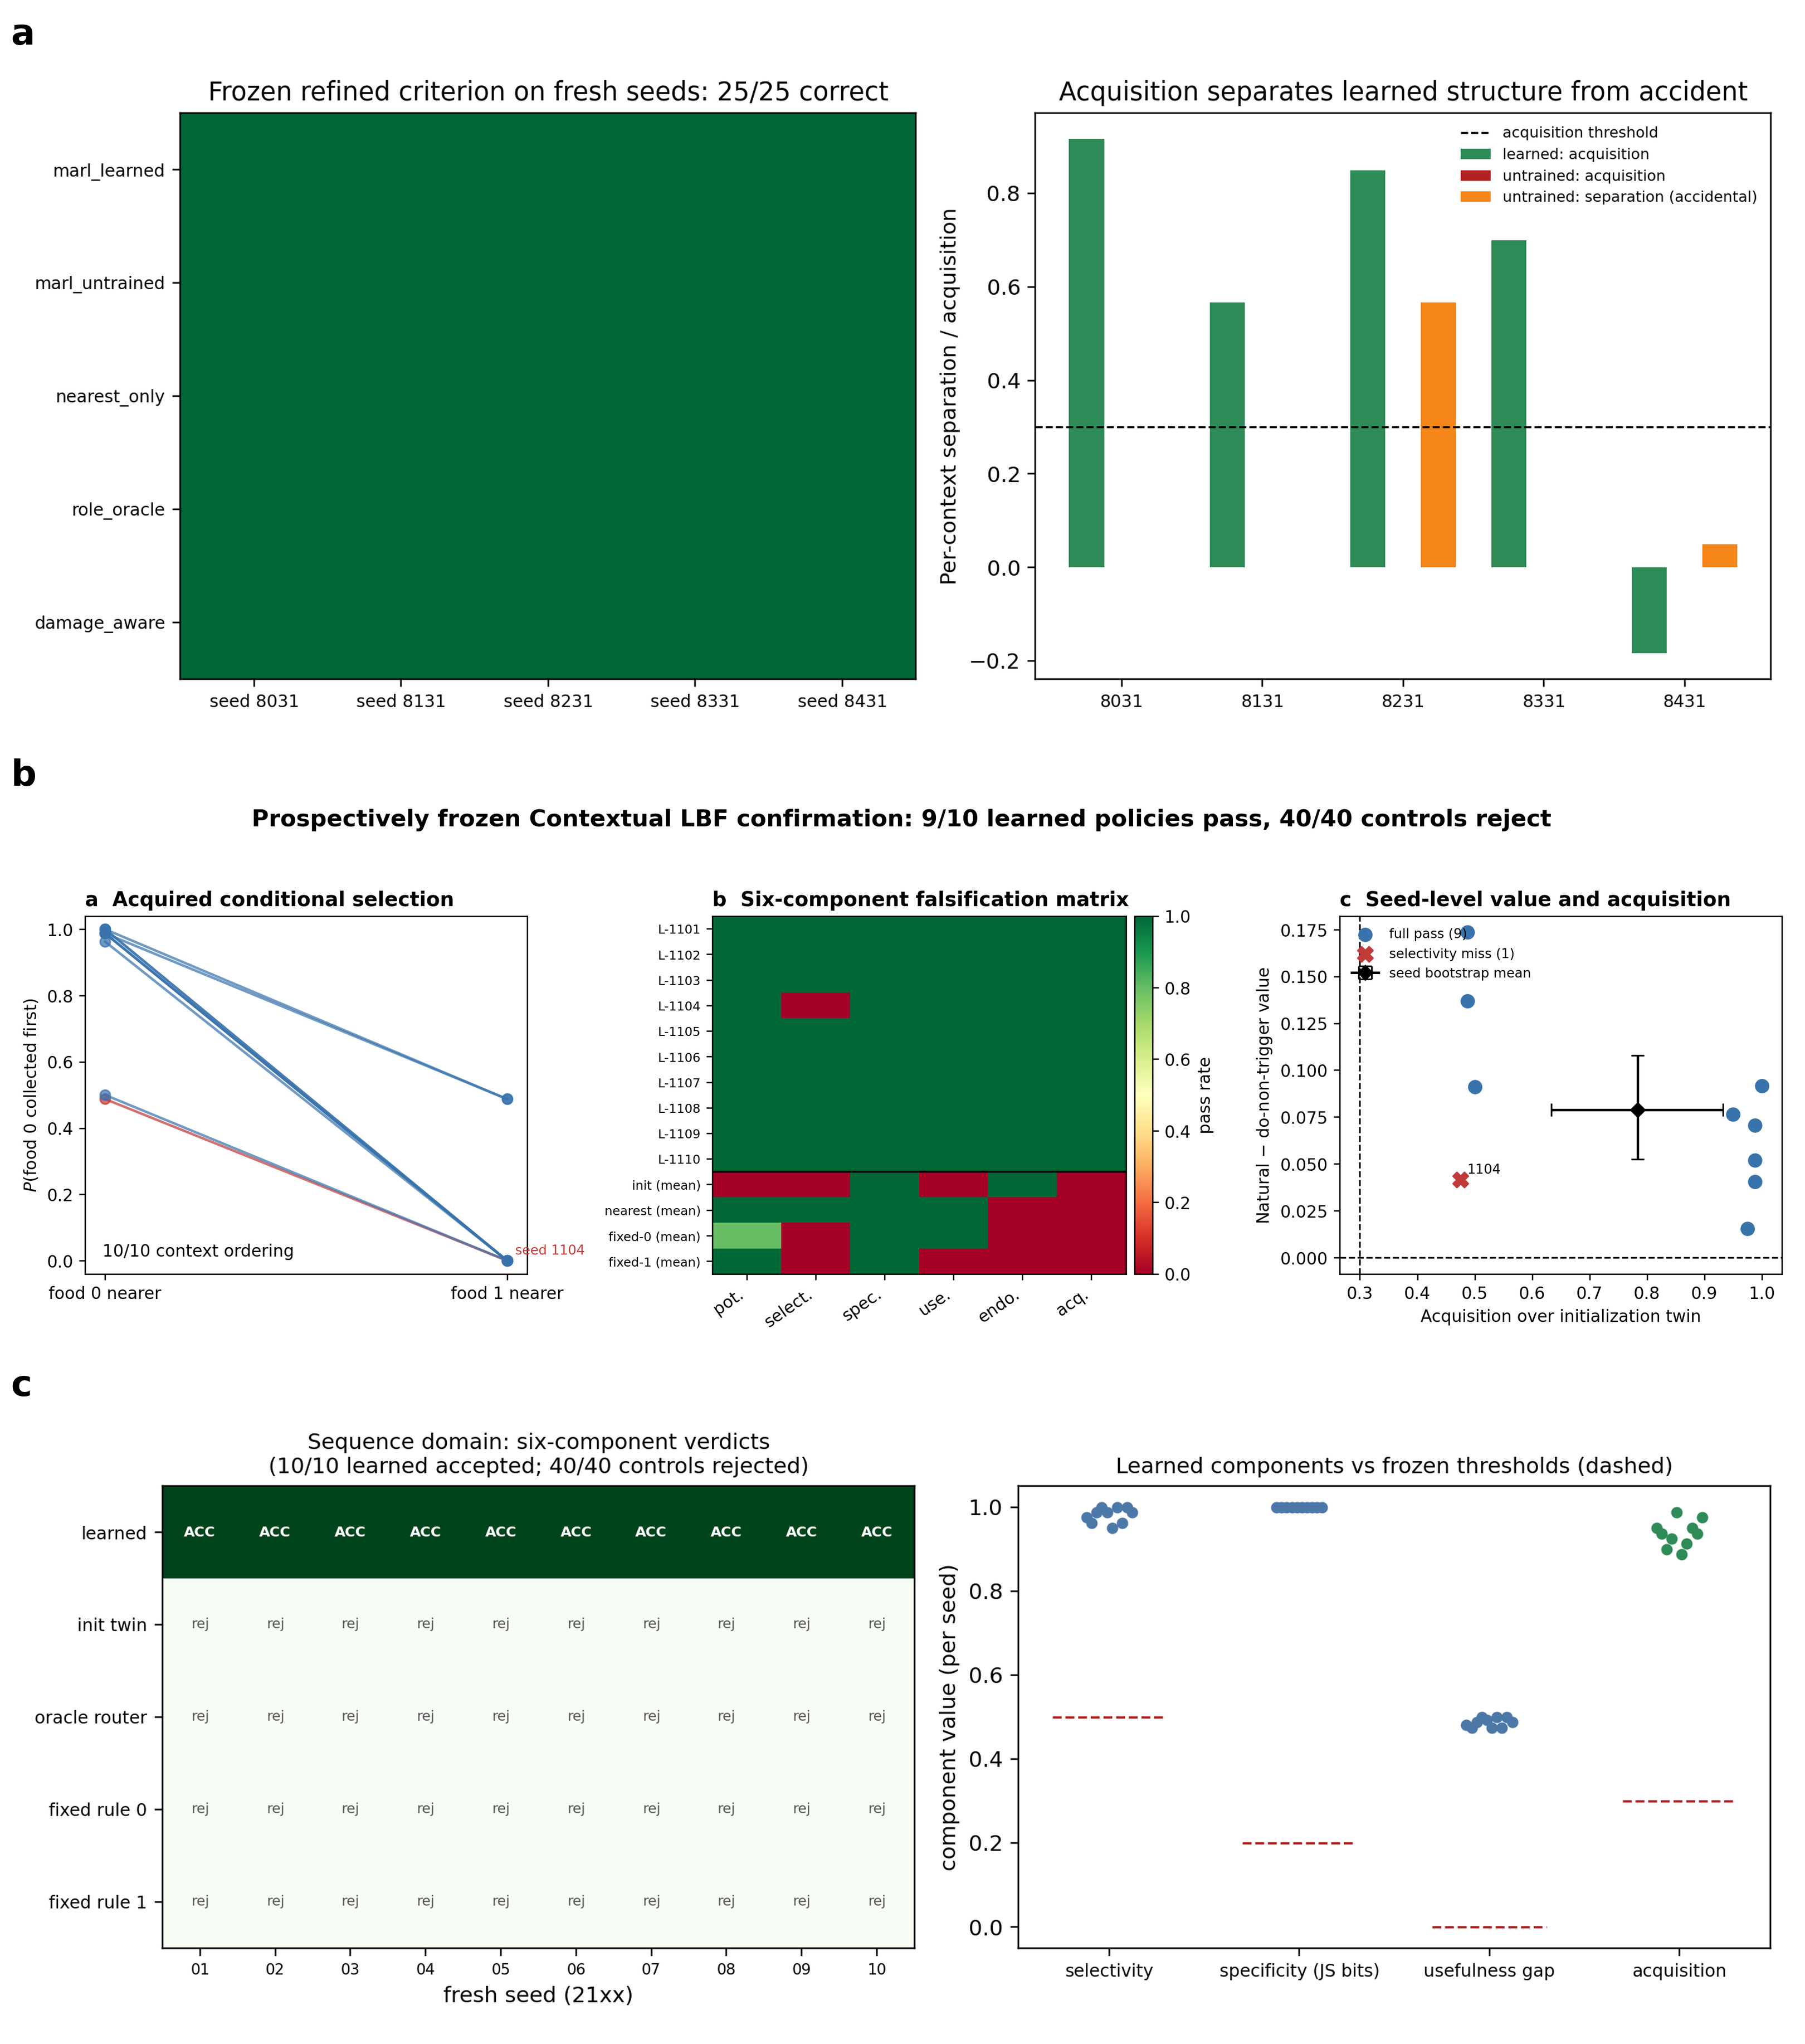
\includegraphics[width=\linewidth]{main_fig3.png}
  \caption{\textbf{The full six-component criterion confirms in three
  system families under frozen thresholds.}
  \textbf{a}, External swarm: refined out-of-sample confirmation,
  25/25 fresh verdicts across five policy seeds, with measured
  acquisition against initialization twins.
  \textbf{b}, Contextual Level-Based Foraging: 9/10 fresh learned
  policies pass all six components (retained miss: seed 1104
  selectivity $0.4875<0.5$); 40/40 initialization and scripted
  controls reject; the competent team-nearest controller fails exactly
  endogeneity and acquisition.
  \textbf{c}, Latent-context sequence model (causal transformer,
  next-token training only): 10/10 fresh seeds accepted, 40/40
  controls rejected (left); per-seed component values clear every
  frozen threshold (right). Thresholds are identical across the three
  domains and were frozen before each confirmatory run.}
  \label{fig:domains}
\end{figure}

This domain also carries the observer, rollout and model-error audits;
we state their conclusions here and their designs, numbers and
retained misses in Methods and Extended Data. The verdict does not
need a hand-made possibility space: machine-partitioned and
cross-fitted basins (four clustering methods on low-level trajectories
only) reject 60/60 controls under every method and agree with the
hand-basin protocol on $95.7\%$ of verdicts, and 13,000 adversarial
random partitions manufacture zero acceptances. A single
\emph{semantics-free} recipe---bag-of-opaque-tokens plus raw numeric
summaries, standardized, $k$-means with $k$ chosen by silhouette,
byte-identical code and hyperparameters---then reproduces the verdicts
across structurally unrelated domains: 8/9 systems on the gridworld
battery with both predeclared positives accepted, 18/18 verdicts and
15/15 control rejections in the collective-control domain, alongside
the stored 95.7\% CLBF agreement. Anyone can compute the possibility
space; the one battery disagreement (a control whose potential the
semantics-free partition inflates by resolving contract-irrelevant
micro-variation) is the residual observer-dependence living exactly
where the refinement guarantee says it must. The verdict is not an
artifact of one observer: under a second plausible contract and a
seven-contract ensemble, all control verdicts are invariant negatives
(60/60 and 420/420), the structural layer agrees on 14/15 learned
seeds, and every learned flip is conservative and concentrated in the
declaredly value-relative usefulness component (Extended Data
Fig.~\ref{fig:ed-dualobs})---structural collapse travels across
reasonable contracts, adaptive qualification is relative to the
declared value, exactly as the definition states. Openness is not
decoding noise (near-greedy rollouts keep every learned seed above
threshold; one diffuse-model prediction failed and is retained), and
verdicts from learned world models replacing the simulator are
reliable when training data is adequate---with the registered
ensemble-disagreement decidability rule failing on shared bias
(retained) and a disclosed coverage-augmented follow-up eliminating
every silent wrong verdict at the cost of conservatism.

\textbf{A sequence-domain full-criterion test.}
To test the protocol beyond embodied RL, we froze a latent-context
sequence task for a small causal transformer trained only by
next-token prediction: the context is never labelled, the valued
continuation rule differs by context, decoding interventions force or
forbid the first continuation token, and an initialization twin
supplies acquisition. Across ten fresh seeds, learned transformers
pass all six components (10/10), all 40 controls reject, and
seed-bootstrap lower bounds are positive for usefulness ($0.481$) and
acquisition ($0.918$) (Fig.~\ref{fig:domains}c). One route prediction
failed informatively: the deterministic oracle router is
intervention-inert, so it fails specificity and usefulness in addition
to provenance. A frozen generalization audit reproduces the boundary
pattern of Contextual LBF; marker positions outside the training range
collapse selectivity. The sequence domain is a controlled next-token
setting, not a claim about natural language.

\textbf{A public third-party environment, preregistered externally.}
Every environment above was built or configured by us. The strongest
remaining objection---that the criterion works only in author-designed
worlds---is answered in Overcooked-AI, a public, unmodified
coordination benchmark~\cite{carroll2019}. The full protocol
(layout pair, training recipe, trigger, basins, both observer
contracts, thresholds copied unchanged from the frozen criterion, and
five predictions OC-1--OC-5) was frozen with a \emph{public external
timestamp} before any confirmatory seed was launched; the run script
refuses to start without asserting that the timestamp exists. Twelve
self-play PPO seeds were then trained on a mixed pair of layouts
(5$\times$10\textsuperscript{6} steps each), with four controls per
seed. All five registered predictions passed (Extended Data
Fig.~\ref{fig:ed-overcooked}): learned policies are accepted on all
six components on 8/12 seeds (registered line 8/12); all 48 control
verdicts are rejections, with the layered failure routes---the
scripted role pair and its behavioural clone are competent but fail
endogeneity and acquisition, twins and untrained pairs fail
selectivity and usefulness; the trigger direction matches the pilot on
12/12 seeds; the declared second contract never rescues a twin
(12/12); and the primary seed-level inference is unambiguous, a
positive usefulness do-contrast on 12/12 seeds (exact sign test
$p=2\times10^{-4}$). The four rejected learned seeds fail
selectivity---they pot in both layouts at similar rates---which is the
correct verdict for a policy that did not develop context-selective
structure, not a miss of the protocol. The continuous record, assembled
read-only with a declared value scale, agrees without seeing the
verdicts: every accepted seed has a positive adaptive score, all 48
controls sit at zero, and the four rejected seeds rank strictly below
every accepted seed on structural score ($0.653$ max vs $0.695$ min,
no overlap).

\textbf{Collective control.}
A supplementary family reconstructs the structure of crowd-scale
collective control (the Twitch-Plays-Pok\'emon phenomenon: thousands
of humans steering one avatar invented a context-dependent
vote-aggregation convention) in a system where every component is
measurable: forty noisy voters drive one avatar, the system's action
is the aggregation mode itself, and a meta-controller is trained on
value alone. All 50 control verdicts reject with exactly the declared
routes---blanket majority-voting fails potential (forced convergence),
blanket anarchy fails usefulness through falls (the historical
counterfactual, reproduced by do-block on 10/10 seeds), and the
hand-scripted switcher and its clone fail exactly endogeneity and
acquisition. Two registered predictions failed and are retained (7/10
learned acceptances against a registered 8/10, all three rejections
being context-blind blanket democracy; graded rather than binary
selectivity), and two design pilots are disclosed (Supplementary
Information). The historical event itself is observational-scale: no
do-operator or twin exists, exactly the scope boundary
Table~\ref{tab:scope-map} declares.

The rejections themselves obey the framework. In two independent
domains, roughly a third of seeds learn a context-\emph{blind}
convention and fail exactly selectivity---so we froze a bifurcation
battery asking whether the blind convention is a lawful competing
attractor. Manipulating the cost of the coordinated mode over five
levels (ten fresh seeds each), the selective-seed fraction moves from
$0.1$ to $0.9$--$1.0$ across the point where the \emph{measured} value
gap between the two conventions (computed from scripted policies,
no learner involved) changes sign, and the gap's sign predicts the
majority basin at 4/5 grid points---the single miss being the
transition region itself (gap $+0.12$). Applying the usefulness
algebra of Proposition~\ref{prop:usefulness} to convention selection
thus predicts \emph{which} training outcomes the certificate will
reject, before training. One registered prediction failed and is
retained: an early-training snapshot does not predict the final
convention basin (chance level; the basin is decided late), so the
bifurcation is forecastable at the population level but not, at this
resolution, for individual seeds. A follow-up battery locates the
decision (five further misses retained across it and its disclosed
margin re-measurement; Supplementary Information): at the population
level the convention space never collapses---fifty seeds settle into a
stable $26/22/2$ split, a bifurcation rather than a universal
attractor---and the deciding variable is not hazard learning at all.
Both conventions end with strong, indistinguishable preferences at the
hazard state; on 24/24 seeds with no overlap, what separates them is
the \emph{open-ground} state, where selective seeds discover that the
cheap uncoordinated mode suffices and blind seeds never do. The
certificate's selectivity rejections thus track a late, stochastic
discovery event in the low-stakes context---measured, not
hypothesized.

\textbf{The framework forecasts.}
Definitions postdict; mechanisms predict. Applying
Proposition~\ref{prop:usefulness} with the closed-form payoffs of the
parametrized gridworld yields derived boundaries \emph{before
training}: behavioural onset of the trigger at goal reward $G = 5$,
usefulness sign change at $G = 9$, second onset at $G = 11$
(boundaries registered in advance). Independent learners trained at
$G \in \{3,5,7,9,11,13,16\}$ then reproduced the derived phase structure:
no structure for $G \le 5$; a selective-but-harmful phase at
$G = 7$---the wrong-selector pattern arising \emph{naturally} from
payoffs, rejected via usefulness as the framework requires; and
accepted emergence above the $G = 9$ analytical usefulness boundary.
The primary registered run matched all four non-tie grid points; three
independent-seed replications matched 11/12 non-tie points ($91.7\%$),
with one false acceptance at $G=7$. The outer phases were stable
(reject at $G\le5$, accept at $G\ge13$ in 3/3 seeds); registered tie
points $G\in\{5,9,11\}$ were not scored. A two-dimensional extension
derives a \emph{non-rectangular} acceptance surface over goal reward
and context mix before training---acceptance requires both a
sufficient payoff and a sufficient context frequency---and 80
independent learners (16 cells $\times$ 5 seeds) match the derived
verdict on 14/15 non-fragile cells by seed majority, reproducing the
predicted interaction (within $G{=}10$ the verdict flips along the
context axis; within low context weight it flips along the payoff
axis). The registered all-cells prediction failed by one cell
($G{=}13$, context weight $0.25$: 2/5 seeds acquire the structure;
low context frequency makes discovery itself stochastic) and is
retained. The experiments support a forecasted transition region
rather than an exact noise-free boundary (Fig.~\ref{fig:marl}b).

\begin{figure}[t]
  \centering
  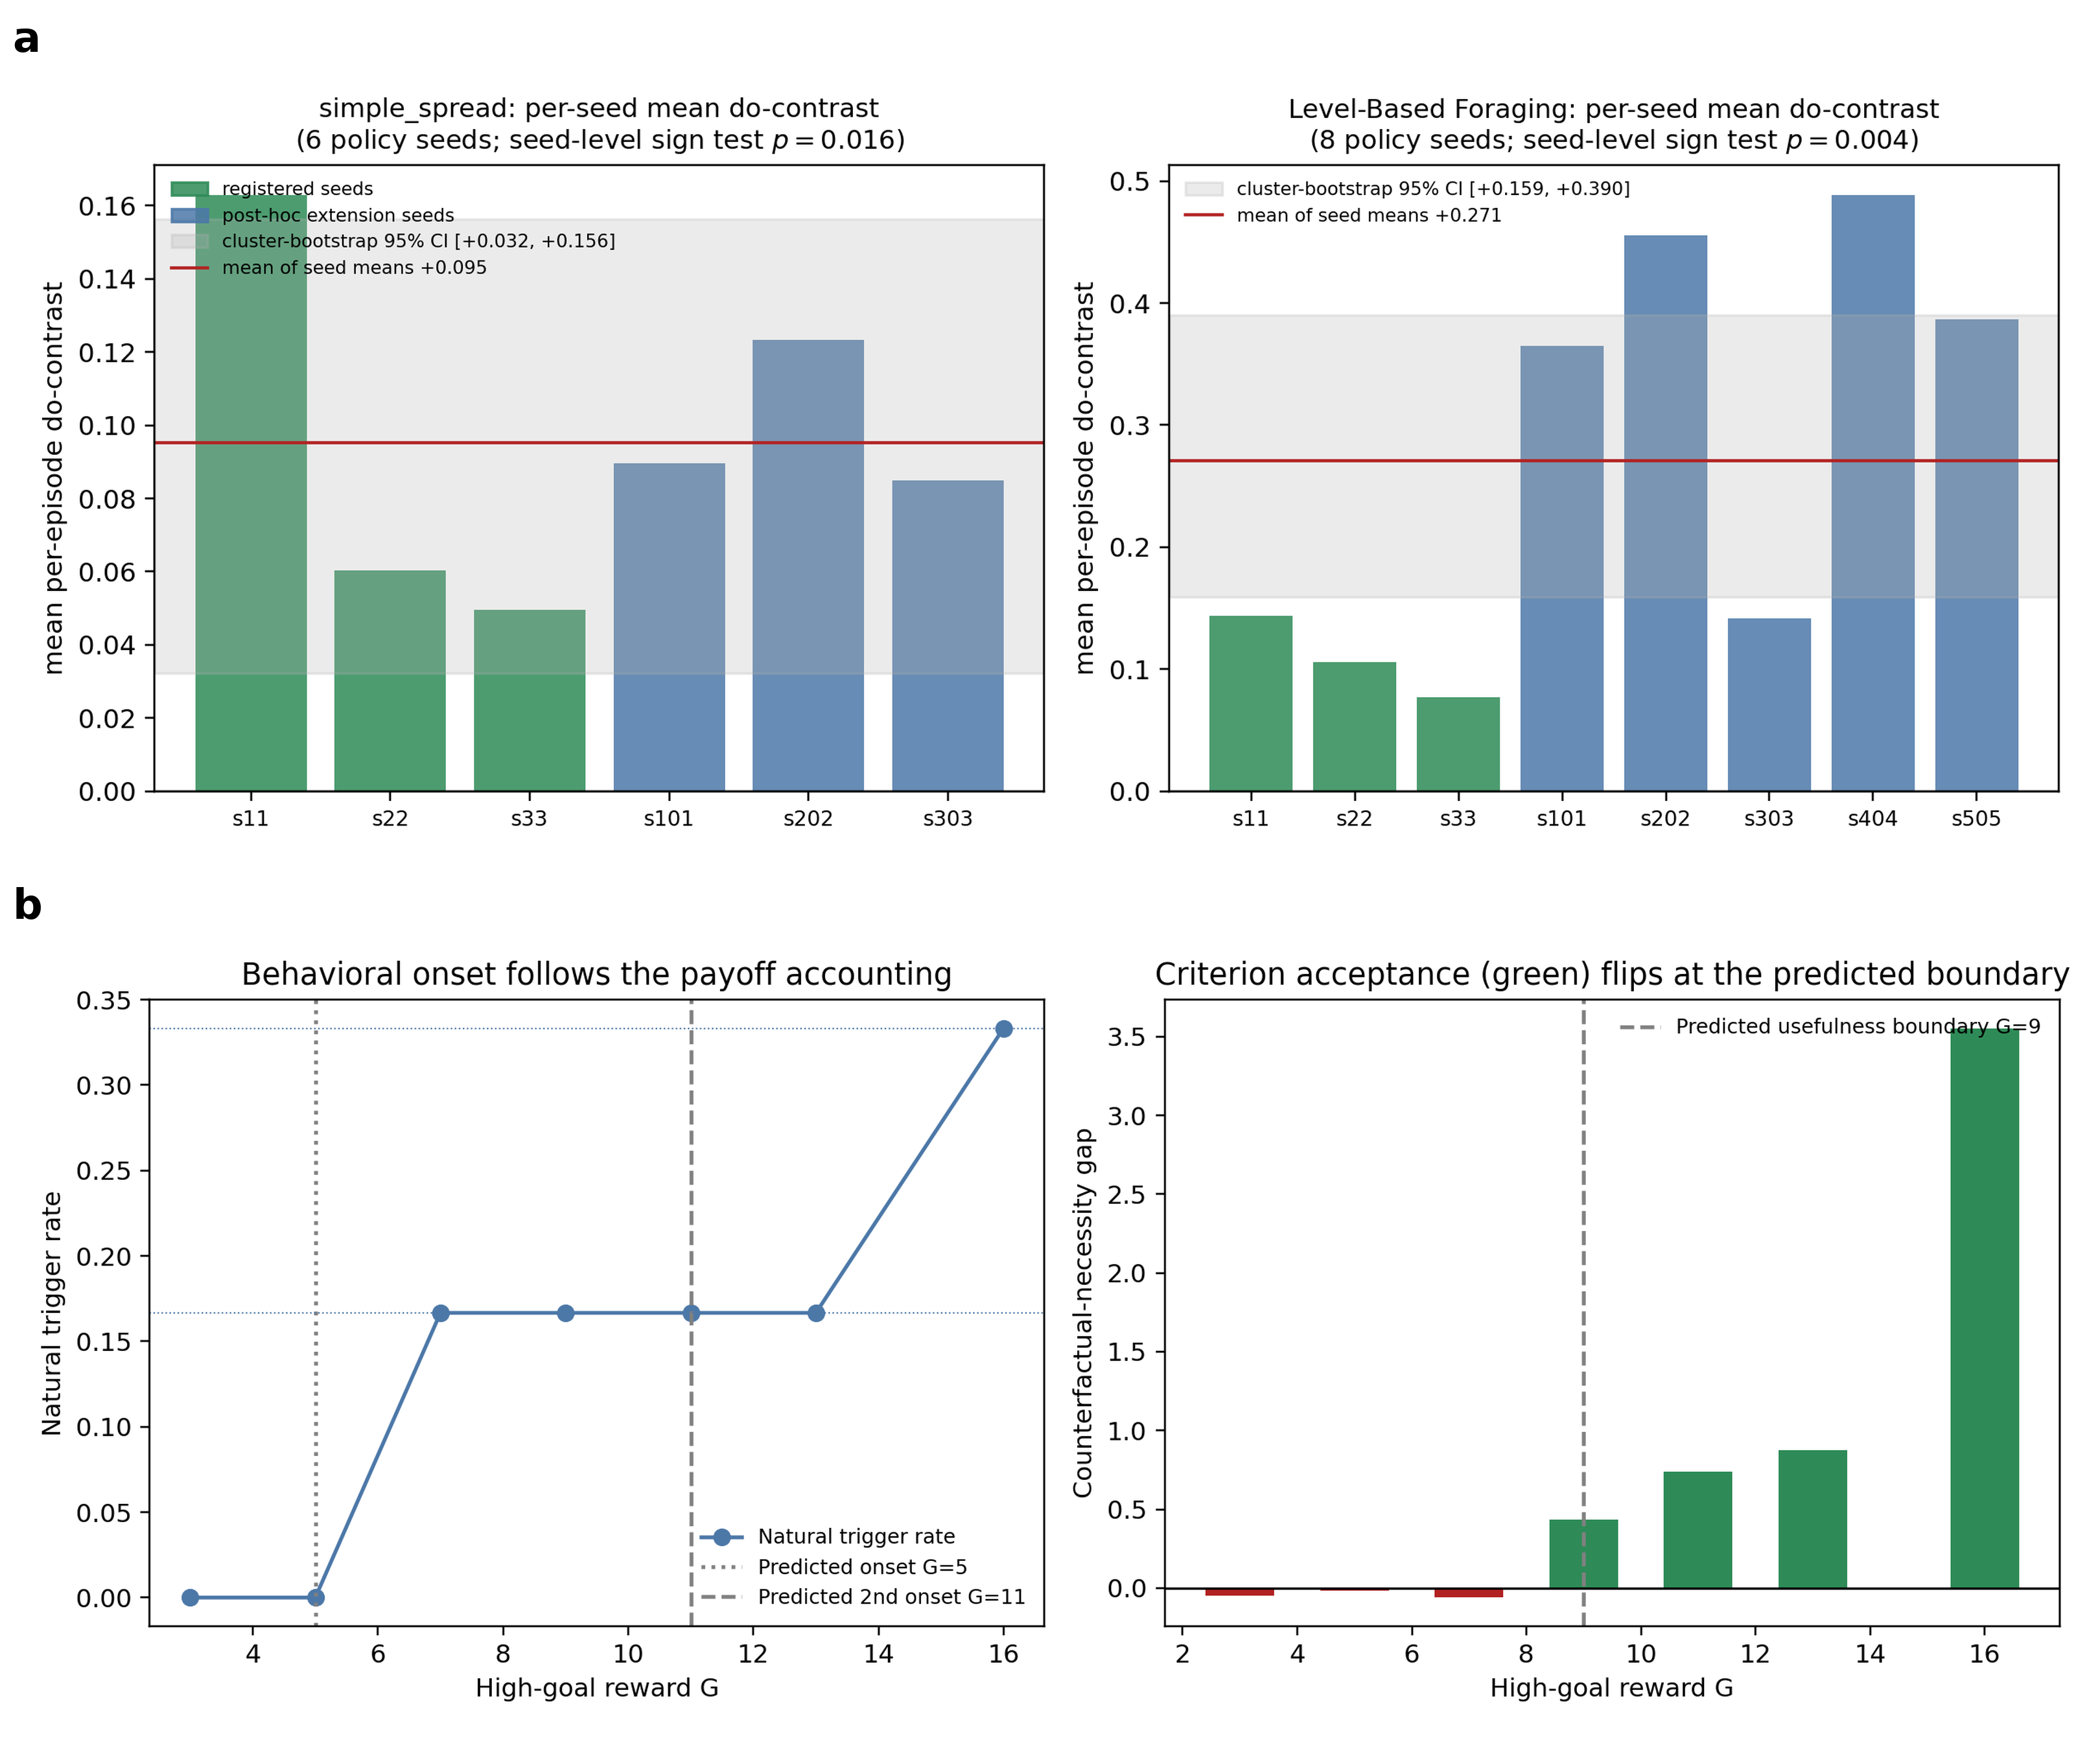
\includegraphics[width=\linewidth]{main_fig5.png}
  \caption{\textbf{Deep multi-agent RL: seed-level inference and
  within-family parameter extrapolation.}
  \textbf{a}, The training-population unit is the policy seed. Per-seed
  mean do-contrasts are positive for all six simple\_spread seeds
  (seed-level sign test $p=0.016$; cluster-bootstrap mean interval
  $[0.032,0.156]$) and all eight LBF seeds ($p=0.004$;
  $[0.159,0.390]$); registered and post-hoc extension seeds are
  distinguished by colour and never pooled silently. Episode-level
  conditional tests and control panels are in Extended Data
  Fig.~\ref{fig:ed-episode}.
  \textbf{b}, The prospective phase-boundary prediction, shown for the
  primary registered run: behavioural onset follows the payoff
  accounting derived before training (left); criterion acceptance
  changes around the predicted usefulness boundary $G = 9$ (right).
  Three independent-seed replications matched 11/12 scored non-tie
  points, with stable outer phases.}
  \label{fig:marl}
\end{figure}

\subsection*{Prospective discovery in uncurated chess play}
\label{sec:chess}

Chess supplies candidate events and an evaluator not produced by the
authors~\cite{mcgrath2022,silver2018}: human annotations nominate
costly candidate key moves, and an engine supplies the counterfactual
future distribution. On 240 externally annotated sacrifices and 120
quiet controls under an internally frozen protocol, the key moves show
the event-level signature (Fig.~\ref{fig:chess}a). They are
\emph{locally costly} (median $-3.0$ pawns against the best reply;
$80.0\%$ $[74.6, 85.0]$ strictly costly), \emph{counterfactually
decisive} ($P(\text{win} \mid \dO{\text{key}}) - P(\text{win} \mid
\dO{\text{best-alternative}})$ mean $+0.539$ $[0.508, 0.570]$, positive
in 240/240 positions), and \emph{not mere openness}: quiet positions
are more open ($+0.764$ bits) yet no single move usefully collapses
them---the opportunity is a property of the state--action pair. All
core conclusions hold in 12/12 robustness cells over temperature,
depth, basin thresholds and a classical engine (Extended Data
Fig.~\ref{fig:ed-episode}). One frozen prediction failed
informatively: the behaving policy's future does not improve after the
key move because the engine prices the move into its own
baseline---$P_t(\text{win})$ is a martingale---and the identical
failure appeared independently in the deep-MARL win-shift prediction
above, forcing the do-contrast
principle stated in the Introduction.

Recovery is not discovery, so a separately frozen protocol sampled 400
uncurated positions per month from public dumps (population filters
only), scored them with the shallow observer alone (potential and the
future-basin do-gap between the depth-4 first and second candidate
moves), and labelled them afterwards with a deep-search referee that
never feeds back into the scores. All four frozen predictions passed
in both months (Fig.~\ref{fig:chess}b): the do-gap ranks
value-critical decisions at AUROC $0.730$ and $0.725$, beats tactical
($0.635$) and material ($0.589$) baselines, and the frozen flag lifts
precision $2.5\times$ and $3.0\times$ over base rate with median
flagged potential $1.9$ bits. Because movers repeat within a month,
inference is also reported at the mover-cluster level: the cluster
bootstrap gives AUROC intervals $[0.615, 0.829]$ and $[0.613, 0.834]$,
wider than position-level intervals but excluding chance by a clear
margin. The engine-native eval-gap baseline is
not distribution-stable ($0.762\to0.652$ across months) while the
do-gap is unchanged. Four referee-family checks bound the remaining
circularity, two passing and two retained as informative failures. A
classical (pre-NNUE) referee leaves the signal intact (AUROC $0.743$
and $0.669$), and mover-cluster bootstrap intervals exclude chance. An
engine-free realized-outcome referee is directionally consistent
(humans play the shallow-best move far more often at flagged
positions, $0.53$ vs $0.34$ and $0.43$ vs $0.27$, with positive
realized-score gains) but its registered interaction is an
underpowered null (permutation $p=0.54$; one decision $20$--$60$ plies
before the end is washed out by subsequent play at these rating
bands). A different-lineage engine referee (Toga~II, Fruit family)
fails the frozen transfer rule ($0.663$ and $0.534$; retained): its
compressed evaluation scale yields $3$--$5$ positives per month and
degrades every predictor including the engine-native baseline, so the
check cannot separate predictor non-transfer from weak-referee label
noise. A lineage-independent referee of comparable strength remains
open (\texttt{CHESS\_DISCOVERY\_PREREGISTRATION.md}).

\begin{figure}[t]
  \centering
  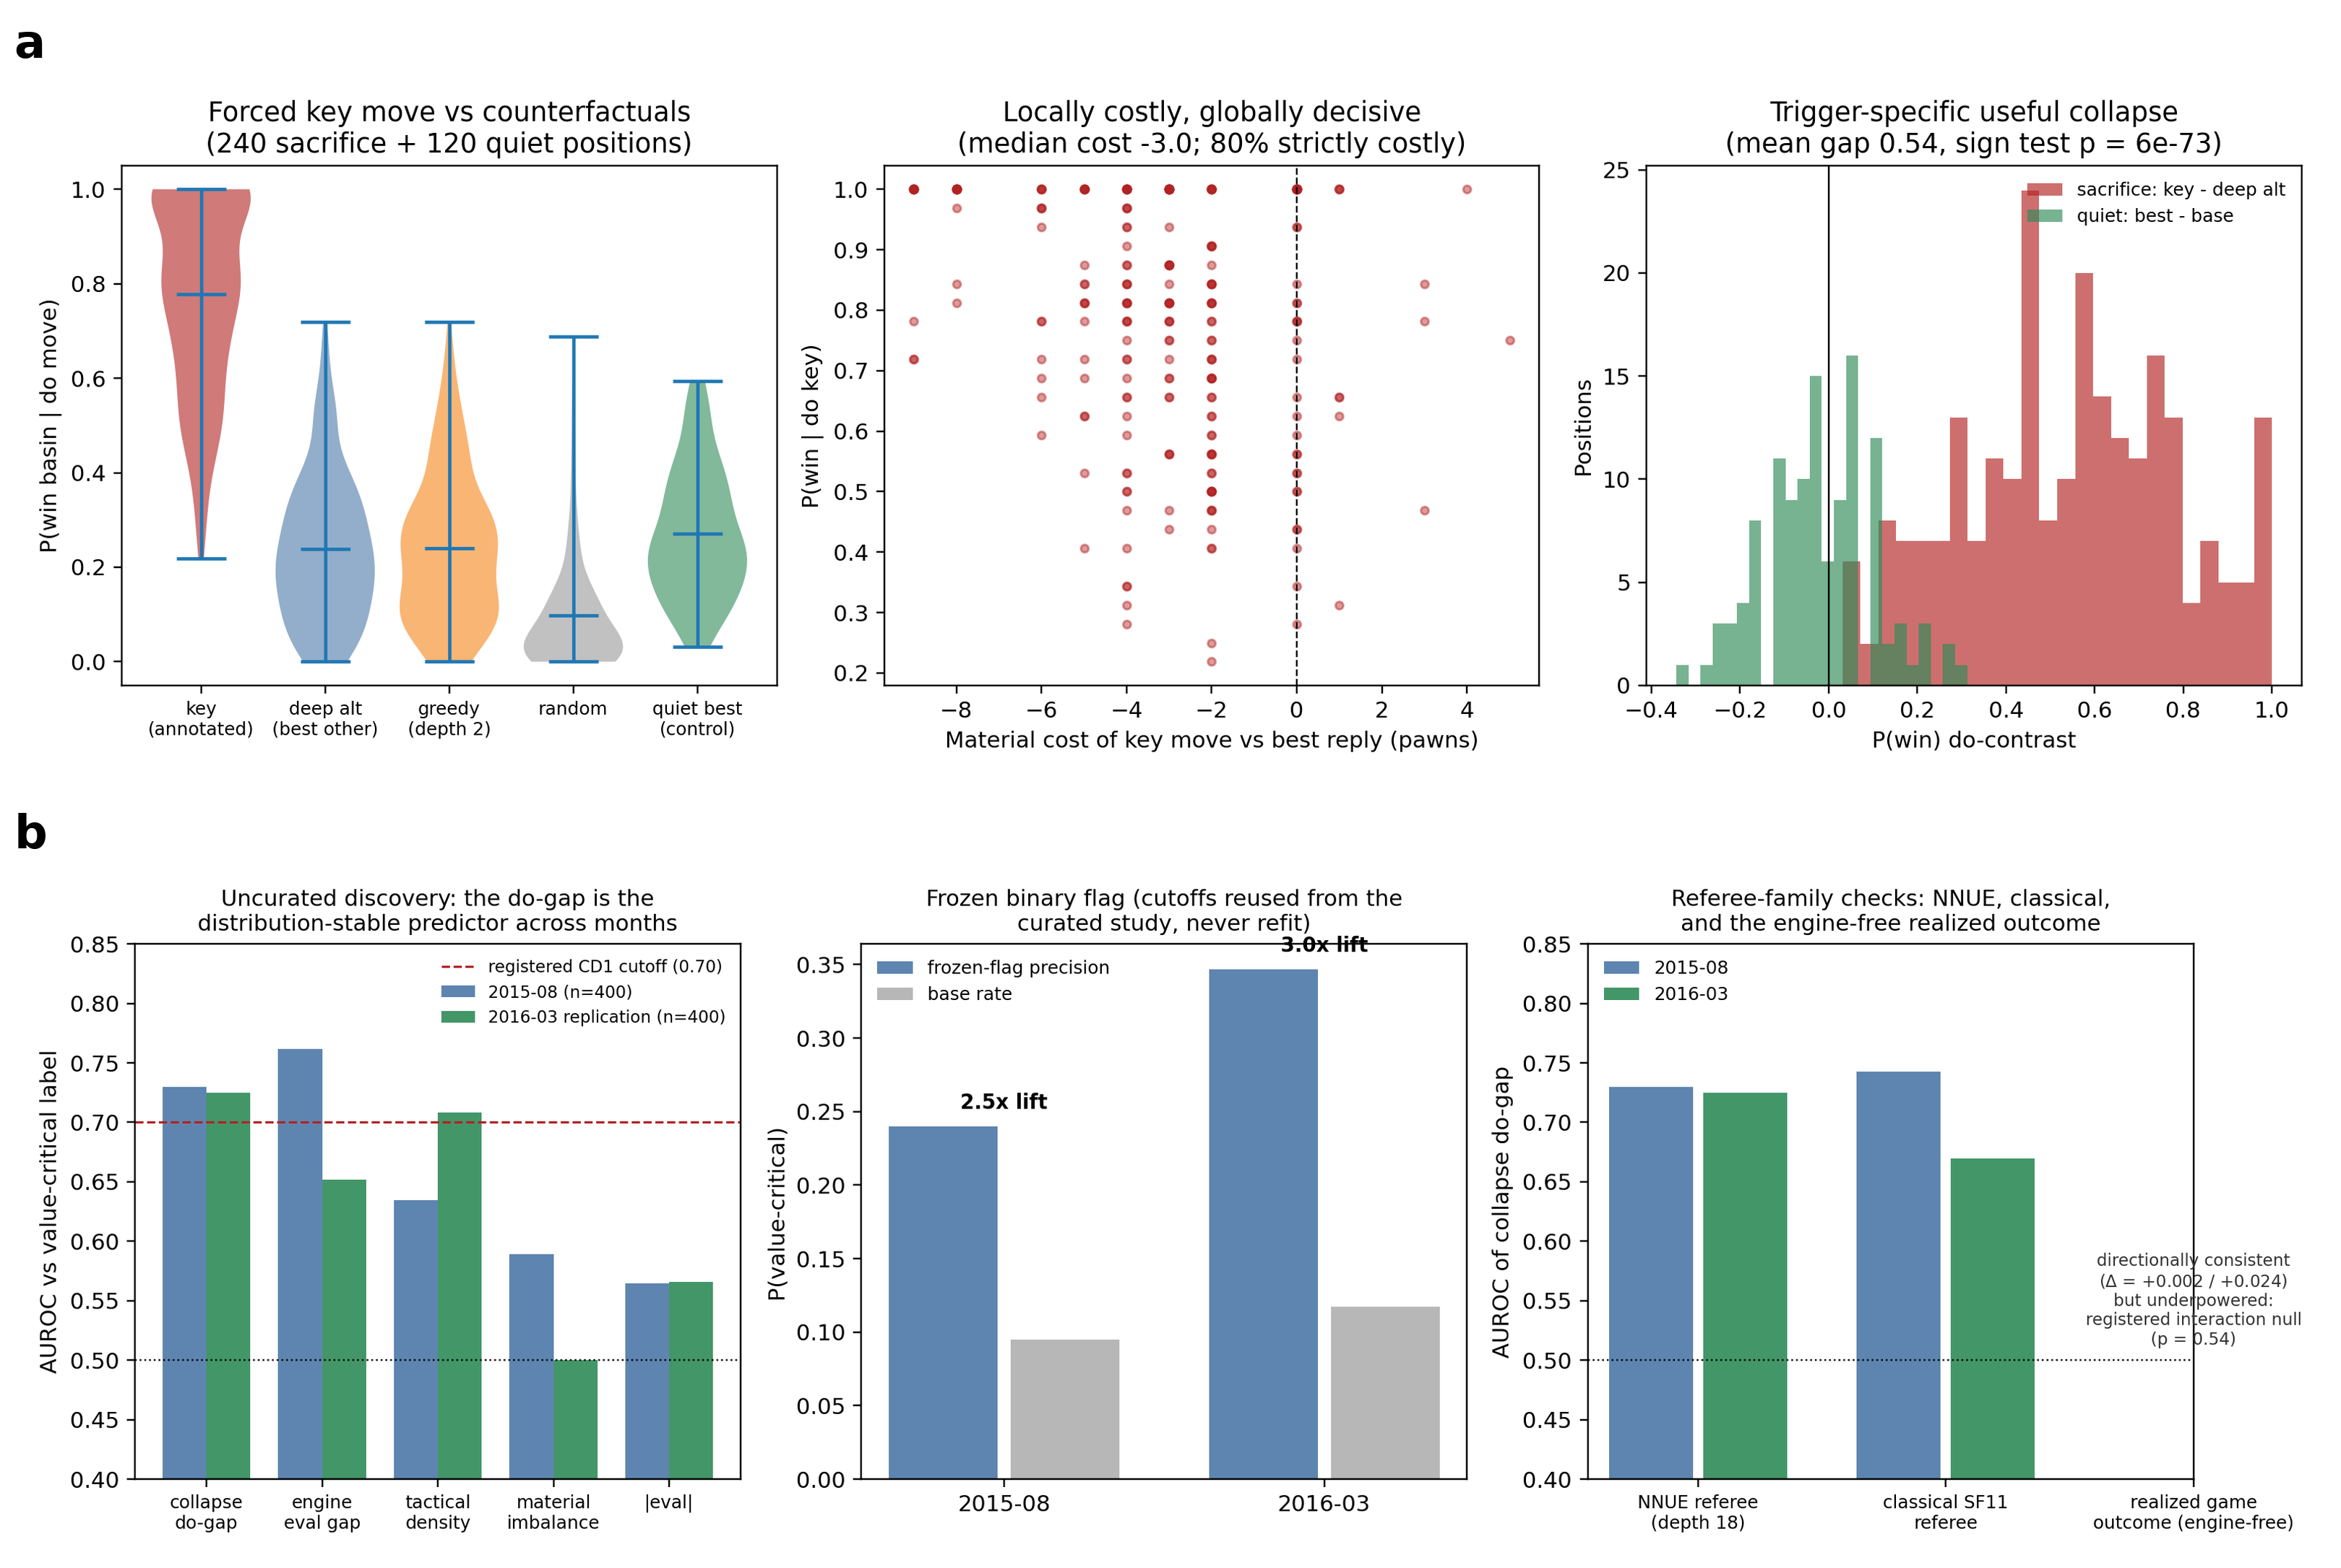
\includegraphics[width=\linewidth]{main_fig4.png}
  \caption{\textbf{Chess: event-level recovery on curated positions and
  prospective discovery on uncurated months.}
  \textbf{a}, Curated recovery: $P(\text{win-basin} \mid
  \dO{\text{move}})$ for the annotated key move vs.\ counterfactual
  alternatives across 240 sacrifice and 120 quiet positions (left);
  the key move is locally costly---median $-3$ pawns vs.\ best
  reply---yet globally decisive (middle); the do-contrast distribution
  separates sacrifices from quiet controls, mean gap $+0.54$ (right).
  \textbf{b}, Uncurated discovery under a separately frozen protocol:
  the collapse do-gap ranks value-critical decisions above tactical,
  material and eval-magnitude baselines in both months and is the
  distribution-stable predictor (left); the frozen binary flag lifts
  precision $2.5\times$/$3.0\times$ over base rate (middle); referee
  families---NNUE, classical SF11, and the engine-free realized game
  outcome---agree in direction, with the realized-outcome interaction
  registered as an underpowered null (right). Acquisition is not
  tested in this domain; estimator/engine robustness cells are in
  Extended Data Fig.~\ref{fig:ed-episode}.}
  \label{fig:chess}
\end{figure}

\subsection*{Prior emergence signatures as low-dimensional projections}
\label{sec:unification}

\begin{proposition}[Coverage and insufficiency of audited signatures]
\label{prop:coverage}
Let $\mathcal{P} = \{ P(\tau \mid c, \dO{w}) \}$ be the intervened
family of trajectory laws over contexts $c$ and interventions $w$
(including none), together with the observer's declared value,
representation, macro-feature and micro-decomposition maps. Then:
\emph{(i)~Derivability.} Each audited emergence quantity---
performance jump (Wei et al.), representation jump, Hoel's exact EI
and CE, Rosas' exact $\Psi$, and PID synergy---is a deterministic
functional $Q = F_Q(\mathcal{P})$, obtained by coarse-graining $\tau$
and/or restricting the intervention set, then applying a fixed
information-theoretic or metric map.
\emph{(ii)~Audited verdict insufficiency.} None of these scalar
functionals, under either its published sign rule or a
hindsight-optimal one-sided threshold, reproduces all predeclared
labels on the battery. This is an empirical statement about the
declared testbed and candidate families, not a universal ranking
theorem.
\end{proposition}

Derivability alone is weak---any statistic computed from a
sufficiently rich family is a functional of it. The content is the
conjunction of (i) with (ii) and the transfers above, and the
framework predicts \emph{when} each signature agrees or fails:
performance jumps are bounded symptoms of collapse
(Proposition~\ref{prop:pinsker}), with grader-dependence exactly
Schaeffer et al.'s critique~\cite{schaeffer2023}; EI intervenes
uniformly, so it cannot see which states the system itself selects and
is sign-blind to value; $\Psi$ reads behavioural marginals, so forced
or wrongly-selective coordination scores highly (its exact top scorer
is the wrong-selector); and when a converged policy prices its trigger
into the baseline, observational value change is a martingale while
the do-contrast remains nonzero---observed independently in chess and
deep MARL. Table~\ref{tab:unification} summarizes each projection and
its measured blind spot.

Each projection also carries a measured \emph{agreement condition}
under which it coincides with the full verdict: performance jumps
agree when value gain, selectivity and provenance co-occur (the
learned positives); representation jumps agree when the moved
distribution is also a useful collapse (Prop.~\ref{prop:pinsker}
witnesses the converse failures); $\Psi$ agrees when coordination is
both learned and correctly context-gated; EI-style efficacy agrees
when the macro-partition is the verdict-carrying one. The battery's
counterexamples are exactly the systems that break each condition
while satisfying the others.
The scope of the claim is precise: \emph{covered} means
derivable-and-audited on systems with an explicit trajectory law and
value structure, within the declared candidate families. We do not
claim that $\Psi$ or EI are wrong in their home use cases (quantifying
macro predictive structure, or intervention-level compression); the
claim is that \emph{as emergence verdicts} they are projections that
discard the verdict-carrying information---the value sign, the
conditional selectivity, and the provenance of the collapse---and that
the layered episode criterion adds structure that no audited
projection, singly or in fitted combination, retains.

\begin{table}[t]
\centering\small
\caption{\textbf{Prior emergence signatures as projections of
$P_t(B)$, each with a measured blind spot.} All numbers from our runs;
rival thresholds are hindsight-optimal (best case for the rival).
Chess percentages: fraction of 240 externally annotated positions
where the signature ranks the key move first.}
\label{tab:unification}
\begin{tabular}{>{\raggedright\arraybackslash}p{0.25\linewidth} >{\raggedright\arraybackslash}p{0.25\linewidth} >{\raggedright\arraybackslash}p{0.42\linewidth}}
\toprule
\textbf{Prior signature} & \textbf{What it reads off $P_t(B)$} & \textbf{Measured blind spot (witness)} \\
\midrule
Performance jump~\cite{wei2022} & usefulness only, no provenance &
accepts the reward-shaped system; misses latent conditional ability
(hindsight acc.\ 0.800) \\
\addlinespace[2pt]
Representation jump & projection bounded by collapse (Pinsker)
(Prop.~\ref{prop:pinsker}) & direction-, provenance-, and
strength-blind: harmful decoy same jump as accepted positive; noise
$13.7\times$ larger; acc.\ 0.900; chess 5.4\% \\
\addlinespace[2pt]
PID synergy / $\Psi$~\cite{rosas2020} (\emph{exact} $\Psi$ computed) &
joint structure of the collapsed state & exact $\Psi>0$ scores 0.3;
top scorer is the wrong-selector ($+0.59$); best threshold must invert
the published sign and still misses the conditional positive \\
\addlinespace[2pt]
Causal emergence, EI~\cite{hoel2013} (\emph{exact} EI computed) &
macro intervention efficacy & exact CE $<0$ on all 10
enumerated chains; best threshold = trivial classifier (0.8), misses
both true positives; proxy's top scorer was the reward-\emph{shaped}
system \\
\addlinespace[2pt]
Metric-artifact critique~\cite{schaeffer2023} & grid-resolution
sensitivity of jumps & \emph{confirmed} from the mechanism side: our
tail-facts results show abruptness is metric- and grid-dependent;
burst is a measurement anchor, not a definition component \\
\bottomrule
\end{tabular}
\end{table}

% ============================================================
\section{Discussion}

The evidence is not flat, and the paper's weight rests on a stated
hierarchy. \emph{Decisive}: the controlled battery with exact rival
forms and equal-freedom baselines; the externally timestamped
Overcooked-AI confirmation; the pre-derived phase boundaries; the
prospective chess discovery. \emph{Supporting}: the three built
full-criterion families, the generator calibration and axioms, the
observer and provenance audits. \emph{Boundary-setting}: the process
proxy's grid-resolution failures, the persistence and generalization
limits, the contract-relative value verdicts. \emph{Failed and
retained}: thirty-six registered predictions, none repaired in place.
A reader who accepts only the decisive tier already has the paper's
claim; the rest raises confidence and marks edges.

The substrate~\eqref{eq:root} is agnostic to the domain of the
possibility space, and two instantiations cover the field's classic
intuitions. \emph{Temporal collapse}: a locally costly or silent act
whose meaning arrives later, when it proves counterfactually
necessary---chess sacrifices are the purest case (local cost $-3$
pawns, do-contrast $+0.54$), and the MultiBERTs NPI result (collapse
at 20k, usefulness at 40k) shows the same shape at training scale.
\emph{Spatial collapse}: a joint basin no individual can reach or hold
alone, certified by single-agent do-blocks degrading the joint
outcome---the operational content of ``the whole exceeds the parts''
without the synergy machinery the exact-form audit shows cannot carry
a verdict. The duality is presentation, not new theory: both are
contractions of one future distribution.

The spatial case carries an exact identity that formalizes two folk
intuitions and one measured blind spot (machine-verified; Methods).
The joint contraction relative to the independence null,
$C_{\mathrm{spatial}} = \sum_i H(B_i) - H(B_1,\dots,B_N)$, \emph{is}
the total correlation of the agents' futures~\cite{watanabe1960,
mcgill1954}, the quantity integration-style measures build
on~\cite{tononi1994}. Populations feel more emergent because the open
possibility space grows linearly with $N$ under independence, so the
collapse available to coordination scales with the group; and
coordination is candidate emergence precisely because it contracts
the joint future space until each individual is predictable from the
others. But the identity also delimits: a deterministic script
attains the \emph{maximal} total correlation, and two mechanistically
different generators with the same joint law are
indistinguishable---structural collapse is provenance-blind as a
matter of mathematics, which is why synergy-flavoured detectors
accept scripted coordination on our battery and why the adaptive
layer, not a better structure statistic, is what separates them.

The same vocabulary classifies the field's textbook exemplars, with
five frozen expectations all met (Methods). In Boids
flocking~\cite{reynolds1987,vicsek1995}, within-episode heading
contraction and the measured three-bird total correlation both rise
monotonically with the alignment coupling ($0.00\to1.64$ and
$0.04\to2.70$ bits), and decoupling the alignment channel mid-episode
shifts the final basin law by a full bit at high coupling while doing
nothing at zero coupling---structural collapse, counterfactually
load-bearing, but \emph{not} adaptive emergence: the dynamics are
prewired and nothing is acquired. Schelling
segregation~\cite{schelling1971} shows the same class with a tipping
signature: the do-freeze contrast is load-bearing only near the
tipping threshold ($0.33$ bits at $\tau=0.7$, zero below), because
below it the system reaches its basin before the intervention can
matter. And Conway's Life~\cite{gardner1970} marks the substrate
boundary exactly: fifty replays of one soup give one future
($H(\text{final} \mid \text{init}) = 0$; the future was never open),
and with no action channel the action-attributable collapse is zero
by Proposition~\ref{prop:bridge}---gliders are deterministic pattern
formation, outside the adaptive scope for a stated reason rather than
by fiat.

These reductions assemble into an explicit type lattice with
per-dimension \emph{analytic} ground truth, guarding against the
circularity of validating an instrument only on its own generator.
Four universal coordinates---non-additivity $N$ (co-information,
analytic on logic gates: XOR exactly 1 bit, majority-3 exactly
$0.434$), interaction dependence $D$ (structure loss under
marginal-preserving surrogate decoupling), causal autonomy $A$
(macro-minus-micro effective information, exact on enumerated
chains), and robustness $R$ (recovery ratio after irrelevant
perturbation)---define \emph{weak emergence} as their joint
satisfaction, with \emph{causal} ($A>0$), \emph{adaptive} (acquired;
this paper's certificate) and \emph{functional} (signed value) tiers
above it, and philosophical strong emergence declared outside the
empirical framework rather than treated as a higher score. Thresholds
were calibrated on Boolean gates, exact Markov chains and constructed
processes only, then frozen and applied blind to families the
calibration never saw: supercritical Kuramoto oscillators classify as
weak emergence and subcritical ones reject, Conway-glider dynamics
classify as weak but not adaptive---exactly Chalmers' canonical
assignment---and a stored learned convention classifies as adaptive
(4/4). An eight-row adversarial matrix (common-driver synchrony,
central controllers, redundant copying, transient coincidences,
static patterns, thresholded pseudo-abilities, harmful congestion)
fails each imposter on the predicted dimension, with harmful
congestion correctly \emph{accepted} as weak emergence with negative
value (8/8). Three rounds of specification errors in the battery's
own truth tables were caught by its exact computations before any
blind system was scored, and are retained in the ledger.

A recent no-go result sharpens what any collapse- or higher-order-based
criterion must show: a common, time-varying environment can generate
synergy-dominated (negative O-information) higher-order structure with
no interaction at all~\cite{envdriven2026}, so higher-order
\emph{statistics} do not imply higher-order \emph{interaction}. We
reproduce this in its strongest form and show the criterion survives it
(Methods; \texttt{emergence\_irreducibility.py}). A deterministic common
cause ($X_1{=}e_1$, $X_2{=}e_2$, $X_3{=}e_1{\oplus}e_2$) is
\emph{distributionally identical} to a genuine three-way role-lock---both
have total correlation $1$ bit, O-information $-1$, and irreducible
higher-order connected information $C_{\mathrm{irr}}=\mathrm{KL}(P\,\|\,P^{(2)})=1$
bit beyond the pairwise maximum-entropy model. No statistic of the joint
distribution separates them; the framework does, two agreeing ways:
conditioning on the environment ($C_{\mathrm{irr}\mid E}=0$ for the common
cause versus $1$ bit for the role-lock) and the do-operator on the
coupling ($D=0$ versus $1$). Strength is graded by \emph{reducibility},
not magnitude: across five systems the rank correlation between total
contraction and $C_{\mathrm{irr}\mid E}$ is non-positive, the
largest-contraction system (redundant consensus, $2$ bits) has
$C_{\mathrm{irr}\mid E}=0$, and a consensus matched to the role-lock's
contraction still separates from it by irreducibility and signed value
(IR-1--6, all passing). This also demotes co-information $N$ itself to
necessary-but-not-sufficient---exactly the no-go's lesson---leaving the
interventional pair ($C_{\mathrm{irr}\mid E}$, $D$) load-bearing, and it
places the criterion between causal emergence~\cite{hoel2013,
hoelce2}, higher-order interaction models~\cite{pithon2025} and
multi-agent learning without coinciding with any of them.

Because the possibility space is the joint-action branch set rather than
the outcome, the criterion also separates mechanisms that reach an
\emph{identical} outcome. Four three-agent systems---a central
controller, a common environment, independent coincidence, and
endogenous local feedback---matched on the final structure and on
single-agent marginals are, for the three that reliably form it,
distributionally identical (uniform over the valid role-lock,
$P(Z){=}1$); no joint statistic separates them. The interaction-broken
counterfactual $P_{\mathrm{broken}}$ (cut agent--agent coupling while
keeping marginals, environment and controller) does: only local feedback
shows collective constraint $C=H(P_{\mathrm{broken}})-H(P_{\mathrm{real}})=1.585$
bits, reorganization $\mathrm{JSD}=0.459$, endogenous macro gain
$M=+0.667$ and irreducibility $C_{\mathrm{irr}\mid E}=1.585$; the two
externally driven systems give $0$ on all four, and independent
coincidence is rejected on persistence ($R=0.30$). Notably the
joint-action entropy \emph{drops} ($3.17$ versus $4.76$ bits) while the
macro capability \emph{rises}---emergence reorganizes micro freedom into
macro capability rather than merely lowering entropy (CC-1--5,
Methods).

The closest existing frameworks share parts of this architecture.
Semantic information~\cite{kolchinsky2018} also combines intervention
with a viability-style value, but scores the information a system
\emph{has about} its environment; our criterion scores a
\emph{structure the system forms}, adding contextual selectivity,
explicit future-basin collapse, acquisition against an initialization
twin, and a cross-domain protocol with frozen thresholds.
Empowerment~\cite{klyubin2005,salge2014} and causal path-entropy
forces~\cite{wissnergross2013} value \emph{keeping} futures open; this
framework identifies when a selective, valuable \emph{contraction},
acquired during learning, should be recognized as adaptive emergence.
Bayesian surprise~\cite{ittibaldi2009} supplies the substrate quantity
itself; none of its uses attach provenance, selectivity or value
direction, which is where the layered criteria live.

Of the $\sim$259 internally frozen predictions, forty-six failed
(nineteen before this revision, plus the realized-outcome interaction,
the second-contract value flips, the strength-gradient suddenness
ordering, the weak different-lineage referee, the diffuse rollout
model, one two-dimensional forecast cell, the bias-blind world-model
error proxy, the constant-series calibration rule, the structure-only
class-separation rule, the early-magnitude prediction battery, the
generator's off-diagonal rule, two convergent-validity endpoints, the
two crowd-domain misses, the bifurcation snapshot rule, the
meta-collapse commitment rules, and the universal-recipe,
blind-demonstration and coordinate-battery specification misses
reported here); none
were discarded or re-thresholded post hoc. The failures carry the paper's
sharpest lessons. Abruptness proved metric- and grid-dependent,
confirming the metric-sensitivity critique~\cite{schaeffer2023} from
the mechanism side and consistent with quantized-computation accounts
of scaling~\cite{michaud2023}; two failures independently exposed the
martingale principle for converged systems; and the acquisition
component itself was added after a random network passed marginal
selectivity by accident, then excluded the untrained control on every
subsequent fresh seed.

The contribution is a scoped measurement framework, not an
observer-free metaphysical definition. The full protocol is validated
where every component is measurable (swarm, Contextual LBF, sequence
model); the battery supplies targeted exclusions and exact
rival-formalism evaluations within declared candidate families; chess
supplies event-level recovery and prospective discovery but no
acquisition; public checkpoints supply a resolution-limited process
instrument, never a full verdict. We do not claim that all emergence
in nature is possibility collapse, that prior definitions are special
cases of ours, that frontier-scale language emergence is solved, or
that the proxy adjudicates ``true'' abruptness. Acquisition
deliberately restricts the verdict to structure acquired during
learning: prewired coordination and architecture-induced transitions
can be structural collapses under Definition~\ref{def:structural} but
sit outside the adaptive verdict, and harmful collapse is
representable rather than denied. The battery labels are designed
diagnostic controls, not third-party ground truth; most frozen
protocols are author-maintained, hash-anchored records without
external timestamps, and one confirmation---in a public, unmodified
third-party environment---carries an external timestamp that predates
every measurement and passed all five of its registered predictions.
Under
declared, auditable observer contracts, useful possibility collapse
can be measured, falsified and transferred, with structural verdicts
stable across plausible contracts and value verdicts explicitly
contract-relative.
The collapse studied here is statistical---a contraction of the rollout
future distribution driven endogenously by the system's own actions or
training dynamics---and carries no quantum connotation.

For machine intelligence, the framework turns ``did an ability
emerge?'' from a curve-reading exercise into an intervention-aware
measurement programme: a common trajectory-law substrate with measured
blind spots for each prior projection, a conservative layered protocol
where triggers, values, interventions and initialization twins are
available, a separate velocity audit for public checkpoint series, a
prospective-discovery test on uncurated data, and a negative-control
practice in which frozen failures are retained and delimit scope. This
is the sense in which possibility collapse unifies the audited uses of
emergence: not by erasing their differences, but by placing them on
one future-distribution object and showing which additional evidence
turns a collapse into an adaptive-emergence verdict.

% ============================================================
\section*{Methods}
\small

\subsection*{Scope of each empirical instrument}
Table~\ref{tab:scope-map} maps every evidence family to the instrument
it supports and the claim it can carry.

\begin{table}[t]
\centering\scriptsize
\caption{Scope of each empirical instrument. ``Full'' is reserved for
settings in which all six components are measurable.}
\label{tab:scope-map}
\begin{tabular}{>{\raggedright\arraybackslash}p{3.0cm}>{\raggedright\arraybackslash}p{3.5cm}>{\raggedright\arraybackslash}p{8.2cm}}
\toprule
\textbf{Evidence family} & \textbf{Instrument} & \textbf{Scope and claim supported} \\
\midrule
Controlled gridworld & five informative episode components &
Action do-contrasts; forced constructions lack an informative
initialization twin. Supports exclusion and threshold audit. \\
External swarm & full six-component criterion &
Action do-contrasts and initialization twins. Supports fresh-seed
full-criterion confirmation. \\
Contextual LBF & full six-component criterion &
Balanced latent geometry, action do-contrasts, initialization twins and
ten independent policy seeds; five additional post-confirmation seeds
reported separately. Supports second-domain confirmation and robustness. \\
Latent-context sequence model & full six-component criterion &
Next-token-trained transformer; decoding do-interventions and
initialization twins; ten fresh seeds. Supports third-domain
confirmation in the sequence modality. \\
Non-contextual deep MARL & potential + counterfactual usefulness &
Action do-contrasts across policy seeds; not a full verdict. Supports
cross-task mechanistic transfer. \\
Human chess & event-level strategic test &
Forced engine alternatives; no acquisition measure. Supports external
candidate/event transfer. \\
Grokking and public checkpoints & four-component process proxy &
No action-level intervention; uses training provenance. Supports
acquisition-process transfer. \\
\bottomrule
\end{tabular}
\end{table}

\subsection*{Proofs of the root identities}
\emph{(0a)} Expand the definition:
$\sum_m P(m) \sum_\tau P(\tau \mid m) \log \frac{P(\tau \mid m)}{P(\tau)}
= \sum_{m,\tau} P(m,\tau) \log \frac{P(m,\tau)}{P(\tau)P(m)} = I(\tau; M)$.
\emph{(0b)} If $M$ is deterministic with cells $A_m$, then
$P(\tau \mid A_m) = P(\tau)/P(A_m)$ on $A_m$ and $0$ elsewhere;
substituting, the log-ratio is the constant $-\log_2 P(A_m)$ and the
conditional mass sums to 1.
\emph{(0c)} Apply the data-processing inequality to the deterministic
channel $g: \tau \mapsto B$; JS is a $f$-divergence-based mixture of
KLs and inherits the inequality.
Numerical verification: \texttt{verify\_theory\_bounds.py}
(MI identity gap $<10^{-9}$; rarity law exact to $<10^{-9}$;
basin JS $0.90 \le$ trajectory JS $1.00$ on do-contrast rollouts).
The spatial-collapse identity ($C_{\mathrm{spatial}} =$ total
correlation $= \mathrm{KL}$ to the product of marginals, $\ge 0$;
independence gives exactly linear growth of the joint entropy in $N$;
coupling monotonicity; script-attained maximum $(N{-}1)\log_2 k$ and
same-law generator indistinguishability) is machine-verified on
20{,}000 random joint laws and exact enumerated families
(\texttt{verify\_spatial\_bridge.py}). The canonical-exemplars battery
(\texttt{canonical\_exemplars.py}) uses minimal standard
implementations: 30 mixing headings with alignment weight and
Gaussian noise (Boids; 3,000 episodes per coupling, 6-sector
discretization for the empirical three-bird total correlation,
do-decouple at mid-episode); a $20{\times}20$ torus with 35\% vacancy
and Moore-neighbourhood tolerance (Schelling; 800 episodes per
threshold, do-freeze at one-sixth horizon); and Life on a
$16{\times}16$ torus (400 random soups, 50 determinism replays of one
soup). Expectations CE-1..CE-5 were frozen in the script docstring
before running; all five passed.

\subsection*{Proof of Proposition~\ref{prop:bridge}}
With a fixed rollout law after the declared step and no unobserved
confounding (an MDP), $P(B \mid \dO{a}) = P(B \mid A{=}a)$, so all
three quantities are standard forms of the mutual information
$I(A;B)$: the contraction form is $H(B)-H(B\mid A)$, the
interventional form is $\mathbb{E}_a \KL(P(B\mid a)\|P(B))$, and the
retrospective form is $\mathbb{E}_b \KL(\pi(A\mid b)\|\pi(A))$, equal
by the symmetry of $I$. A deterministic $\pi$ makes $A$ constant, so
$I(A;B)=0$. The scientific content is the declaration that all
manuscript measurements target the interventional form, with the
identities verified numerically ($10^4$ random systems, max gap
$<10^{-15}$; trained gridworld trigger steps, gap $<10^{-16}$;
\texttt{verify\_bridge\_identity.py}).

\subsection*{Proof of Proposition~\ref{prop:pinsker}}
Write $\Delta(b)=P_t(b)-P_{t-1}(b)$, so
$J_t=\lVert\sum_b \Delta(b)\phi(b)\rVert_2$. For any unit vector $u$,
the scalar function $f_u(b)=u^\top\phi(b)$ has range at most
$\mathrm{diam}(\phi)$. The total-variation duality gives
\[
  \left|\sum_b \Delta(b) f_u(b)\right|
  \le \mathrm{diam}(\phi)\,\TV(P_t,P_{t-1}).
\]
Taking the supremum over unit $u$ yields
$J_t \le \mathrm{diam}(\phi)\TV(P_t,P_{t-1})$. The second step is
Pinsker's inequality with the bit-to-nat conversion
$\KL_{\mathrm{nats}} = \ln 2 \cdot K_t$. Verified at every step of
every trajectory in four training regimes and both grokking
conditions.

\subsection*{Observer refinement and model-error guarantees}
Let $B'$ refine $B$, with $B=h(B')$. Then
$H(B')=H(B)+H(B'|B)\geq H(B)$, and data processing gives
\[
\JS(P_a(B'),P_{a'}(B')) \geq
\JS(P_a(B),P_{a'}(B)).
\]
Thus a coarse-partition Potential or JS-Specificity pass remains a pass
under refinement at the same absolute threshold. If value is
coarse-measurable, $u'(b')=u(h(b'))$, its do-gap is exactly invariant.
Entropy contraction itself is not refinement-monotone because the two
conditional-entropy terms can change in either direction.

For rollout-model laws $Q_a,Q_{a'}$ approximating target laws
$P_a,P_{a'}$, suppose
\[
\TV(P_a,Q_a)\leq\epsilon_a,\qquad
\TV(P_{a'},Q_{a'})\leq\epsilon_{a'},
\]
and $u$ has range $R$. Then
\[
\left|\Delta_P u-\Delta_Q u\right|
\leq R(\epsilon_a+\epsilon_{a'}).
\]
Accordingly, a measured usefulness margin larger than this bound is
stable to the declared model error; without an estimate of the
$\epsilon$ terms the do-gap remains observer-model relative. Finally,
if each signed component margin exceeds its own error bound, the full
conjunctive verdict is stable; a union bound gives confidence at least
$1-\sum_i\delta_i$. Ten thousand random-distribution checks for each
partition/model bound and all 27 bounded-burst checks produced zero
violations (\texttt{observer\_bounds\_verification.json}).

\subsection*{Witnesses for Proposition~\ref{prop:nosingle}}
\begin{table}[h]
\centering\scriptsize
\caption{Illustrative measured witness pairs: accepted and rejected
systems that share, nearly share, or reverse a single-observable
signal. Exhaustive threshold sweeps, rather than each pair alone,
establish the best achievable battery accuracy.}
\label{tab:witnesses}
\begin{tabular}{llll}
\toprule
\textbf{Observable} & $S^{+}$ (accepted) & $S^{-}$ (rejected) & shared/reversed signal \\
\midrule
potential & latent\_conditional ($H_0 = 1.15$) & useful\_habit ($H_0 = 1.11$) & open futures \\
collapse burst & grokking (burstiness 3974) & prewired (28376) & sudden collapse \\
specificity JS & noise\_policy (0.74) & harmful\_decoy (0.65) & trigger-contingent futures \\
usefulness gap & latent\_conditional ($+3.4$) & useful\_habit ($+4.4$) & positive gap \\
representation jump & uncertain-preference bridge & pure-team probe & large $J_t$ \\
causal-emergence EI & latent\_conditional ($+0.71$) & shaped\_process ($+0.93$) & macro beats micro \\
\bottomrule
\end{tabular}
\end{table}
The EI row uses the charitable episodic proxy; the exact-form
computation (below) worsens the failure to the trivial classifier.

\subsection*{Exact rival formalisms}
For each of the ten battery systems we enumerated the policy-closed
Markov chain exactly: state $=$ (mode, context, agent positions,
switch flag, clock), up to $75{,}004$ states, with the learned softmax
policy in closed form; the chain is time-inhomogeneous but exact.
\emph{Hoel EI:} $\EI(T) = I(X_{t+1}; X_t)$ with $X_t$ uniform
(max-entropy interventions) on the exact transition matrix;
$\CE = \max_g \EI(\text{macro}_g) - \EI(\text{micro})$ over a
five-member coarse-graining family including the mechanistically
privileged partitions (mode-collapse, context-collapse,
position-collapse, outcome classes, trivial). Exhaustive search over
all coarse-grainings is super-exponential and is not performed in the
original literature either; the conclusion is stated for this family.
\emph{Rosas $\Psi$:}
$\Psi(V) = I(V_t; V_{t+1}) - \sum_j I(X^j_t; V_{t+1})$ on the pooled
one-step joint of the behavioural occupancy measure, maximized over
four supervenient features $\times$ two micro decompositions (the
first-order practical criterion, as in the original applications;
since verdicts are also evaluated at hindsight-optimal thresholds,
constant redundancy offsets cannot rescue the ordering failures).
Script: \texttt{exact\_prior\_formalisms.py}; output:
\texttt{outputs/exact\_prior\_formalisms.json}.

\subsection*{Internal battery and refinement}
Ten gridworld systems with designed ground truth; 36--96 rollouts per
estimate. Plug-in entropy/JS estimation is consistent with
Miller--Madow bias $O((|B|-1)/n) < 0.09$ bits at the battery setting,
below every margin the verdicts rely on. Estimator robustness: all
qualitative conclusions unchanged across $n \in \{12..96\}$ and probe
temperatures (12-cell grid); registered thresholds sit on wide
accuracy plateaus (one honest edge documented: the noise policy sits
at $H_0 = 0.508$, near the 0.5 potential cutoff). After a registered
failure in which 2/5 external replication seeds accepted an untrained
network on marginal tension, the criterion was refined \emph{under
freezing}: conditional selectivity
$|p_{\mathrm{trig}}(A) - p_{\mathrm{trig}}(B)| \ge 0.5$; acquisition
$\ge 0.3$ separation gain over own initialization. The full
six-component rule was confirmed out-of-sample on 25/25 external
verdicts across five fresh seeds. A fresh internal seed classified
10/10 systems with the five informative components; acquisition was
not scored internally because the forced-behaviour constructions have
no informative initialization twin. The battery systems are designed
diagnostic controls with predeclared labels, not an independent gold
standard; their role is falsification pressure, and the independent
tests are the frozen-threshold transfers, the public-checkpoint and
chess studies, and the fresh-seed confirmations.

\subsection*{Fair multivariate baselines}
Prior-signal baselines receive equal or greater freedom than the
six-component conjunction: AND-rules over one to three prior signals
(representation jump, metric jump, specificity, synergy, EI-style
contrast; each signal with its own hindsight threshold and direction),
an $\ell_2$ logistic regression and a depth-2 decision tree on all
five signals plus the exact EI and $\Psi$ values, and two-component
AND-rules over our own measured components. All models are fitted on
the original battery scores, evaluated by leave-one-out
cross-validation, then frozen and applied to a fresh-seed battery
(seed 7011) whose five transportable prior signals were recomputed
from scratch; the six-component reference on that seed is the stored
confirmation, untouched by this analysis
(\texttt{fair\_baseline\_comparison.py},
\texttt{fair\_baseline\_comparison.json}).

\subsection*{Grokking, induction heads, and scale}
Grokking (modular addition, MLP + causal transformer + attention-only
families): thresholds frozen in the bridge code
(potential $\ge 1.0$ bits; burstiness $\ge 5$; usefulness gain
$\ge 0.2$; endogeneity by design flag); the memorization phase inside
the same run is the sharpest internal control---held-out entropy
$6.6 \to 2.8$ bits with zero accuracy gain, refused by the anchored
window. This mirrors, in our vocabulary, the mechanistic progress
measures that precede the grokking transition~\cite{nanda2023}: the
collapse burst is a provenance-bearing progress measure, not a
performance curve. Induction heads: attention-only transformers on cyclic-repeat
sequences; the two-layer model passes all process-proxy components (copy accuracy
0.987), the one-layer model---which provably cannot implement the
circuit~\cite{elhage2021}---fails usefulness (0.112); 12/12 registered
predictions on fresh seeds. The in-context ability whose collapse we
track is the same one shown to emerge only under bursty, heavy-tailed
training distributions~\cite{chan2022}, consistent with our reading of
it as an acquired---not prewired---collapse.

\subsection*{Public checkpoint series}
MultiBERTs: 29 intermediate checkpoints $\times$ 5 seeds; 288
agreement minimal pairs; random-target controls share the agreement
entropy/KL trace, while shuffled-vocabulary controls perturb the
ability readout and test usefulness under the same public checkpoint
series. Pythia-160m/410m/1B:
21 published checkpoints each, fetched from public Pythia checkpoint
revisions; next-token
distribution at the critical verb position; the same 288-pair
construction (all verb pairs single-token in the GPT-NeoX vocabulary);
tail families scored by mean per-token log-probability
(eval-harness convention; tokenization amendment recorded before any
checkpoint behaviour was observed). For both public series, the
\texttt{train\_acc} and \texttt{test\_acc} columns store the same fixed
evaluation-battery score for compatibility with the bridge analyser;
there is no separate probe-training/test split, and no such independence
is claimed. Conditions within a model seed share checkpoints and probe
construction; the five model seeds provide seed replication, while
paired controls diagnose verdict routes. All predictions and outcomes:
\texttt{MULTIBERTS\_PREREGISTRATION.md},
\texttt{PYTHIA\_PREREGISTRATION.md} and
\texttt{PYTHIA\_SCALING\_PREREGISTRATION.md}. The 1B and 1.4B runs use
official sharded checkpoint revisions verified by a per-revision
SHA-256 audit (all cached revisions pairwise distinct,
\texttt{pythia\_1.4b\_checkpoint\_hashes.json}); byte-range spot checks
confirmed the download source serves content identical to
\texttt{huggingface.co} for locally verified shards. The 2.8B run uses
official sharded revisions after two upstream defects (a duplicated
shard and a mismatched revision) were detected by the hash audit,
quarantined and rebuilt from authentic sources; the earlier 2.8B
mirror output remains quarantined and excluded.

\subsection*{Chess}
240 positions selected by the Lichess \texttt{sacrifice} theme and
rating band 1800--2400, plus 120 quiet controls; futures estimated by Stockfish rollout ensembles
(registered temperature/depth); win/draw/loss basins by centipawn
thresholds; do-operators implemented as forced first moves. Robustness
grid: temperature $\times$ depth $\times$ basin thresholds $\times$
engine (incl.\ classical Stockfish 11). Protocol frozen in
\texttt{CHESS\_PREREGISTRATION.md}; the C5 margin failure and its
martingale post-mortem are recorded there. Statistical intervals treat
positions as independent units and are conditional on the curated
annotation sample; no claim about population prevalence is made.
The realized-outcome referee parses the same public PGN dumps for the
game result and the human move actually played at each scored ply
(never used by any scoring stage); the registered contrast is the
realized-score gain from playing the shallow-best move at flagged
versus unflagged positions, with a 10,000-shuffle permutation test on
the interaction and bootstrap CIs per month; mover-rating balance
between flagged and unflagged positions is reported as a confounder
audit (\texttt{chess\_realized\_outcome.py},
\texttt{chess\_realized\_outcome.json}).

\subsection*{Deep MARL}
\texttt{simple\_spread}: MAPPO, 3 seeds, do-commit/do-block on target
assignment; Level-Based Foraging (LBF, forced-cooperation
\texttt{5x5-2p-2f}): MAPPO-style PPO, 3 seeds, sparse reward;
interventions release on consumption (a
pilot-stage semantic fix recorded with logs before the main run);
probe temperature 6.0 chosen in pilots and stress-tested across
$T \in \{2,3,4.5,8\}$ with frozen success criteria. Detector
comparison on 8 LBF systems includes forced-commit and a hand-coded
cooperating imitation; the round-1 set-composition failure is archived
and the round-2 prediction was frozen before the rerun.
A post-hoc seed extension trained three further simple\_spread and
five further LBF policies with unchanged code and probes
(\texttt{deep\_marl\_collapse\_seed\_extension.json},
\texttt{lbf\_collapse\_seed\_extension.json}); combined seed-level
statistics over $6$ and $8$ independent policies give exact one-sided
sign tests $p=0.016$ and $p=0.004$ with positive cluster-bootstrap mean
intervals $[0.032,0.156]$ and $[0.159,0.390]$
(\texttt{hierarchical\_marl\_analysis\_combined.json}). The extension
sizes were set by a seed-level power simulation from the three
registered seeds (simulated one-sided power at $\alpha=0.05$:
$\ge 0.99$ at $K=5$ for simple\_spread and $\ge 0.89$ at $K=5$,
$\ge 0.99$ at $K=8$ for LBF), recorded in the same analysis file; the
simulation's normality assumption and its dependence on three-seed
effect estimates are stated there. The extension is reported
separately from the registered three-seed runs.

\subsection*{Contextual LBF six-component confirmation}
Base benchmark \texttt{Foraging-5x5-2p-2f-coop-v3} (lbforaging 2.0.0)
with unchanged dynamics, local observations, six discrete actions and
sparse collection reward. A wrapper balances two unlabeled geometric
contexts (food identity 0 or 1 nearer to the team; two interior
layouts per context selected by episode seed; horizon 15); the context
label is never given to any controller. Training: the existing PPO
implementation, 8{,}000 episodes per policy seed, no shaping.
Trigger: food 0 collected first; basins:
$\{\text{win},\text{loss}\}\times\{\text{food-0-first},
\text{food-1-first}\}$; value: discounted mean sparse team reward
($\gamma=0.98$); $\dO{\text{trigger}}$/$\dO{\text{non-trigger}}$:
minimal shared cooperative path/load planners toward the corresponding food,
released once the target is consumed. Thresholds are copied unchanged
from the previously frozen refined criterion. Evaluation: 80 episodes
per context and condition; the training seed is the population unit.
Two disclosed design pilots preceded the freeze and are excluded;
confirmation seeds 1101--1110 were fixed in
\texttt{CONTEXTUAL\_LBF\_PREREGISTRATION.md} (code SHA-256 recorded)
before any confirmation training. The post-confirmation extension
(seeds 1201--1205), the one-at-a-time threshold-sensitivity rescoring
and the hindsight-optimal single-signal audit are post-hoc analyses
stored in
\texttt{contextual\_lbf\_extension\_analysis.json},
\texttt{contextual\_lbf\_threshold\_sensitivity.json} and
\texttt{contextual\_lbf\_single\_signal\_audit.json}.

\subsection*{Strength-gradient battery}
Same benchmark dynamics; rewards defined per provenance (shaped: team
$+2.0\times$[trigger action]; outcome-only: team
$+4.0\times$[rescue outcome]); five seeds each; pattern probability
$p_t = P(\text{sacrifice-rescue basin})$ under near-greedy checkpoint
policies (200 evaluation episodes, Laplace-smoothed);
$C_t=-\log_2 p_t$. Open-space reference: 20{,}000 uniform-random
episodes. Provenance rarity: mean $C_t$ over the first quarter of
training. Predictions ST-1--ST-4 were frozen in the script docstring;
the ST-3 suddenness ordering failed on the 20-point/60k-episode grid
because both provenances complete acquisition inside one checkpoint
interval, and a disclosed fine-grid follow-up (40 checkpoints over
10k episodes) confirms later discovery and higher pre-discovery
rarity for outcome-only while suddenness remains unordered
(\texttt{strength\_gradient\_battery.py},
\texttt{strength\_gradient\_fine.py}).

\subsection*{Dual observer contracts}
The second contract was declared before running: horizon 12,
undiscounted success probability as value, and speed-refined basins
(first-food identity $\times$ completion within 10 steps) that still
resolve the trigger. Any admissible contract must resolve the declared
macro-structure; contracts that erase the trigger identity are
excluded by the measurement contract itself. All 75 stored systems
(15 policy seeds $\times$ 5 systems, confirmation plus extension) were
re-scored with frozen thresholds from saved policy networks and
reconstructed initialization twins; registered predictions DO1--DO3
and the five conservative learned-side flips are recorded in
\texttt{dual\_observer\_contracts.py} and
\texttt{dual\_observer\_contracts.json}.

\subsection*{Learned basins, rollout models and the contract ensemble}
For the machine-partitioned-basin audit, a $k$-means partition ($k=4$,
fixed initialization per seed) is fitted on the pooled natural
episodes of each seed's five systems using behavioural summary
features (first-consumed-food one-hot, foods collected, normalized
episode length); the identifiability rule (mutual information between
cluster and trigger $\ge0.1$ bits) is checked, and only potential and
specificity depend on the partition. The cross-fitted audit uses
low-level features only (padded per-step agent coordinates, per-agent
action histograms, per-step reward sequences), fits on even-indexed
natural episodes, freezes the partition, scores odd-indexed natural
and all do-episodes, selects $k\in[2,8]$ by silhouette on the training
half, and repeats over $k$-means, Gaussian mixture, Ward agglomerative
(nearest-centroid assignment) and PCA-10+$k$-means. For the
rollout-model audit, learned policies and initialization twins are
re-scored under softmax temperatures $0.2$ and $2.0$ with all
thresholds frozen; the epistemic-versus-behavioural rollout
distinction is declared in Terminology, and the IR-2 miss is retained.
The contract ensemble pools the seven stored frozen-threshold
contracts read-only and reports per-system acceptance rates
(\texttt{learned\_basin\_clbf.py},
\texttt{crossfit\_lowlevel\_basins.py},
\texttt{independent\_rollout\_audit.py},
\texttt{contract\_ensemble\_analysis.py}).

\subsection*{Harmful emergence, matched provenance and the 2-D surface}
The learned-harmful construction trains agent 0 on an exploiter reward
($r_0$ plus a bonus when its partner is lured onto the decoy goal);
both value functions ($u_{\mathrm{private}}$, $u_{\mathrm{team}}$)
were declared before training, and predictions HE-1--HE-4 passed 5/5
seeds (\texttt{learned\_harmful\_emergence.py}). The
matched-provenance battery compares a hand script, a tabular
behavioural clone of it, and the shaped and outcome-only learners of
the strength battery, with a disclosed design pilot and predictions
MP-1--MP-5 frozen after it (\texttt{matched\_provenance.py}). The 2-D
phase surface derives per-cell verdicts over goal reward
$G\in\{3,7,10,13\}$ and latent-context weight
$w\in\{0.10,0.25,0.40,0.70\}$ in closed form before training, declares
one fragile cell (predicted margin $0.0625$), and trains 5 fresh seeds
per cell (\texttt{phase\_2d\_prediction.py}).

\subsection*{Continuous profile and calibration}
The profile record and its fixed aggregation live in
\texttt{emergence\_profile.py}: potential normalized by
$\log_2 |B|$; causal magnitude as the do-law JS divergence (bounded
by 1 bit); signed value as $\tanh$ of the do-contrast over a
per-domain scale declared before assembly ($\sigma_V = 5$ gridworld
return units, $0.1$ CLBF discounted-reward units); acquisition as the
clipped structure gain over the initialization twin; abruptness as one
minus the normalized entropy of positive collapse increments (bounded,
thinning-stable). The certificate margin (soft-min over standardized
component margins) measures evidence strength, not phenomenon
strength, and is reported separately. Calibration:
\texttt{profile\_calibration.py} (orthogonal generator grid;
dose--response; the original cross-term rank rule failure is retained)
and \texttt{profile\_existing\_systems.py} (read-only taxonomy
assembly). ``Strong/weak emergence'' is deliberately avoided as
terminology. Ranking stability across the five stored contracts and
the early-profile predictive-validity battery (four outcome-variable
boundary cells, five fresh seeds each, snapshot at 25\% of training)
are scored in \texttt{contract\_ranking\_stability.py} and
\texttt{predictive\_validity.py}; the RS-2 and PV-1..3 misses are
retained.

\textbf{Ground-truth generator and axioms.} The six-knob generator
(\texttt{generator\_calibration.py}) fixes trigger probabilities
$p_1 = \tfrac{1}{2}(1{+}s)$, $p_0 = \tfrac{1}{2}(1{-}s)$, a do-trigger
basin law of declared concentration $b$, a value contrast $v$, a twin
carrying fraction $1{-}q$ of the structure, a logistic collapse path
of steepness $a$, and a perturbation retaining fraction $r$;
dimensions are measured with the full finite-sample pipeline (4{,}000
episodes per condition, three measurement seeds). Predictions
GC-1--GC-5 were frozen in the script docstring; GC-2's exemption-list
error and the $R{\leftarrow}b$ structural coupling are retained as a
miss with a disclosed follow-up. The eight record axioms are verified
in \texttt{verify\_record\_axioms.py} (20{,}000-sample ensembles for
nullity, boundedness, monotonicity, data processing and context
sensitivity; value/provenance separability pinned to GC-4/5;
abstention pinned to the world-model follow-up). The admissible
contract family and the identification-interval report are defined in
\texttt{THEORY.md} and computed in
\texttt{contract\_ranking\_stability.py}. The convergent-validity
battery (\texttt{convergent\_validity.py}, fresh 9800-series seeds,
CV-1 pass, CV-2/3 retained misses) scores component-to-matching-
endpoint prediction with a pooled model and no per-cell refitting.

\subsection*{World-model closure}
Tabular MLE models of $(s,a) \mapsto (s', \text{events}, r,
\text{done})$ are fitted on $K \in \{200, 1000, 5000, 20000\}$
on-policy trajectories (five data seeds per $K$, three policy seeds);
components are recomputed with the model replacing the simulator in
probe rollouts. The registered error proxy was mean pairwise TV
between the five models' natural-basin distributions; WM-1/WM-2
passed, WM-3 failed and is retained. The disclosed follow-up adds an
incomplete-rollout fraction cut of $0.10$; it catches all 20
mismatches but abstains at $K{=}20000$, where forced interventions
still hit unseen state--action pairs in 39--50\% of rollouts
(\texttt{world\_model\_closure.py},
\texttt{world\_model\_closure\_followup.py}).

\subsection*{Overcooked-AI confirmation}
The public benchmark is used unmodified (\texttt{overcooked\_ai},
commit-pinned). Twelve self-play PPO seeds (77001--77012) are trained
on the mixed layout pair (\texttt{cramped\_room},
\texttt{asymmetric\_advantages}), $5{\times}10^{6}$ environment
steps, shared parameters, community shaped rewards annealed to zero
over 60\% of training. The trigger is agent 0 potting first; basins
are (first potter $\times$ delivery); contract A uses sparse team
value at horizon 400, contract B success-indicator value at horizon
300. Controls per seed: initialization twin, scripted role pair,
behavioural clone of the scripted pair, and an independently
initialized untrained pair; thresholds are copied unchanged from the
frozen criterion. The full protocol and predictions OC-1--OC-5 were
frozen with a public external timestamp before any confirmatory seed
was launched; two design pilots are disclosed in the preregistration
(\texttt{OVERCOOKED\_PREREGISTRATION.md},
\texttt{overcooked\_confirmation.py},
\texttt{overcooked\_aggregate.py}).

\subsection*{Terminology and the system boundary}
\emph{Observer contract}: the declared measurement setting---a basin
partition $B=g(\tau)$ that resolves the candidate macro-structure, a
value function, a rollout policy, an intervention set, a time
resolution, and a system boundary. \emph{Trajectory-law family}: the
set of trajectory distributions $\{P(\tau \mid c, \dO{w})\}$ over
declared contexts and interventions. \emph{Collapse} names three
related statistics that the text keeps separate: retrospective
conditioning (Eq.~\ref{eq:root}, bookkeeping only), the within-run
contraction of $\Ptb$, and the interventional divergence between
do-laws (both measured). \emph{Process proxy}: the four-component
checkpoint instrument; its burst component measures acquisition
velocity, not emergence magnitude.

The rollout model requires the same discipline: it is an
\emph{epistemic} choice when it approximates the fixed target
policy's own conditional futures (rollout counts, horizons, mild
decoding changes that preserve the behaving distribution), and it
becomes a \emph{behavioural intervention}---defining a different
system---when it alters the policy's action distribution itself, as
strong temperature inflation does. The rollout-model audit is scored
under this declaration.

The system boundary deserves an explicit statement because endogeneity
depends on it. The contract declares the system to be the policy with
its learned parameters at measurement time; endogeneity holds when the
trigger is selected by that system's own action distribution rather
than forced by the measurement apparatus, and it is deliberately
paired with the \emph{measured} acquisition component, which compares
the same system against its own initialization and therefore does not
rely on a design flag. The pairing has a known boundary: a network
supervised to clone a script would pass acquisition, and the framework
then classifies it as adaptive \emph{with respect to its declared
training signal}---provenance is relative to the declared boundary,
not an absolute property. Reward, architecture and curriculum shape
every learned system; the criterion does not adjudicate those upstream
choices and no claim depends on it doing so.

\subsection*{Statistics and internal protocol freezing}
Sign tests are exact binomial. All headline effect sizes carry 20,000-
resample percentile bootstrap 95\% CIs over their natural independent
units. For chess the position is the independent unit. For deep MARL,
episode-level intervals and sign tests quantify intervention effects
conditional on the three trained policies; policy-seed medians are
reported separately, and the episode-level $p$ values are not used as
population-level inference over training randomness. Confirmatory
stages use author-maintained protocols frozen before their reported
measurements, with outcomes recorded in place. These records are not
third-party registered reports and do not provide an external
timestamp; they are supplied for auditability. The exception is the
Overcooked-AI confirmation, whose full protocol, thresholds and
predictions were frozen with a public external timestamp before any
confirmatory seed was launched
(\texttt{github.com/FanYixiang2000/emergence-prereg}, tag
\texttt{v1.0-overcooked-prereg}, commit \texttt{8415e45},
2026-07-18); the confirmation script refuses to run without an
explicit flag asserting that this timestamp exists. A single-page audit
(\texttt{PREDICTION\_LEDGER.md}) indexes $\sim$259 frozen
verdicts/checks with 46 recorded misses, stratified into four tiers---
roughly twenty primary confirmatory hypotheses (Tier~1), the
replication/transfer hypotheses (Tier~2), diagnostic and mechanistic
predictions (Tier~3), and software/artifact invariants (Tier~4); the
main text's claims rest on Tiers 1--2 only, and the count is a
transparency record, not a sample size---each row pointing to its
primary document. Ledger rows are heterogeneous and dependent, so the
count is not treated as a sample size or combined significance test.
Reported $p$ values test their local contrasts; no family-wise
significance claim is made across the heterogeneous ledger.
When a miss motivated a refinement, the miss remains
counted as a miss; the revised component or threshold is recorded as a
method change and contributes only through later frozen tests on fresh
seeds, public checkpoints, or new task families. Code and outputs
sufficient to regenerate every figure are provided
(\texttt{REPRODUCIBILITY.md}).

% ============================================================
\clearpage
\begin{thebibliography}{99}\small

\bibitem{anderson1972} Anderson, P. W. More is different.
\emph{Science} \textbf{177}, 393--396 (1972).

\bibitem{bedau1997} Bedau, M. A. Weak emergence.
\emph{Philos.\ Perspect.} \textbf{11}, 375--399 (1997).

\bibitem{holland1998} Holland, J. H. \emph{Emergence: From Chaos to
Order} (Addison-Wesley, 1998).

\bibitem{mitchell2009} Mitchell, M. \emph{Complexity: A Guided Tour}
(Oxford Univ.\ Press, 2009).

\bibitem{crutchfield1994} Crutchfield, J. P. The calculi of emergence:
computation, dynamics and induction. \emph{Physica D} \textbf{75},
11--54 (1994).

\bibitem{batterman2002} Batterman, R. W. \emph{The Devil in the
Details: Asymptotic Reasoning in Explanation, Reduction, and Emergence}
(Oxford Univ.\ Press, 2002).

\bibitem{wei2022} Wei, J. \emph{et al.} Emergent abilities of large
language models. \emph{Trans.\ Mach.\ Learn.\ Res.} (2022).

\bibitem{kaplan2020} Kaplan, J. \emph{et al.} Scaling laws for neural
language models. Preprint at arXiv:2001.08361 (2020).

\bibitem{brown2020} Brown, T. B. \emph{et al.} Language models are
few-shot learners. \emph{Adv.\ Neural Inf.\ Process.\ Syst.}
\textbf{33}, 1877--1901 (2020).

\bibitem{bommasani2021} Bommasani, R. \emph{et al.} On the
opportunities and risks of foundation models. Preprint at
arXiv:2108.07258 (2021).

\bibitem{hoffmann2022} Hoffmann, J. \emph{et al.} Training
compute-optimal large language models. \emph{Adv.\ Neural Inf.\
Process.\ Syst.} \textbf{35}, 30016--30030 (2022).

\bibitem{schaeffer2023} Schaeffer, R., Miranda, B. \& Koyejo, S. Are
emergent abilities of large language models a mirage?
\emph{Adv.\ Neural Inf.\ Process.\ Syst.} \textbf{36} (2023).

\bibitem{hoel2013} Hoel, E. P., Albantakis, L. \& Tononi, G.
Quantifying causal emergence shows that macro can beat micro.
\emph{Proc.\ Natl Acad.\ Sci.\ USA} \textbf{110}, 19790--19795
(2013).

\bibitem{hoelce2} Hoel, E. Causal emergence 2.0: quantifying emergent
complexity. Preprint at arXiv (2025).

\bibitem{pithon2025} Emergence of temporal higher-order interactions
from pairwise collaboration. \emph{Commun.\ Phys.} (2025).

\bibitem{envdriven2026} Environment-driven emergence of higher-order
collective behaviour. Preprint (2026).

\bibitem{rosas2020} Rosas, F. E. \emph{et al.} Reconciling emergences:
an information-theoretic approach to identify causal emergence in
multivariate data. \emph{PLoS Comput.\ Biol.} \textbf{16}, e1008289
(2020).

\bibitem{williamsbeer2010} Williams, P. L. \& Beer, R. D.
Nonnegative decomposition of multivariate information. Preprint at
arXiv:1004.2515 (2010).

\bibitem{bertschinger2014} Bertschinger, N., Rauh, J., Olbrich, E.,
Jost, J. \& Ay, N. Quantifying unique information. \emph{Entropy}
\textbf{16}, 2161--2183 (2014).

\bibitem{lizier2018} Lizier, J. T., Bertschinger, N., Jost, J. \&
Wibral, M. Information decomposition of target effects from
multi-source interactions: perspectives on previous, current and future
work. \emph{Entropy} \textbf{20}, 307 (2018).

\bibitem{mediano2021} Mediano, P. A. M. \emph{et al.} Towards an
extended taxonomy of information dynamics via integrated information
decomposition. Preprint at arXiv:2109.13186 (2021).

\bibitem{hoel2025} Hoel, E. Causal emergence 2.0: quantifying emergent
complexity. \emph{Patterns} \textbf{6}, 101472 (2025).

\bibitem{barnett2023} Barnett, L. \& Seth, A. K. Dynamical
independence: discovering emergent macroscopic processes in complex
dynamical systems. \emph{Phys.\ Rev.\ E} \textbf{108}, 014304 (2023).

\bibitem{luppi2022} Luppi, A. I. \emph{et al.} A synergistic core for
human brain evolution and cognition. \emph{Nat.\ Neurosci.}
\textbf{25}, 771--782 (2022).

\bibitem{ganguli2022} Ganguli, D. \emph{et al.} Predictability and
surprise in large generative models. In \emph{Proc.\ ACM Conf.\ on
Fairness, Accountability, and Transparency (FAccT)} 1747--1764 (2022).

\bibitem{srivastava2023} Srivastava, A. \emph{et al.} Beyond the
imitation game: quantifying and extrapolating the capabilities of
language models. \emph{Trans.\ Mach.\ Learn.\ Res.} (2023).

\bibitem{chan2022} Chan, S. C. Y. \emph{et al.} Data distributional
properties drive emergent in-context learning in transformers.
\emph{Adv.\ Neural Inf.\ Process.\ Syst.} \textbf{35}, 18878--18891
(2022).

\bibitem{bialek2001} Bialek, W., Nemenman, I. \& Tishby, N.
Predictability, complexity, and learning. \emph{Neural Comput.}
\textbf{13}, 2409--2463 (2001).

\bibitem{power2022} Power, A., Burda, Y., Edwards, H., Babuschkin, I.
\& Misra, V. Grokking: generalization beyond overfitting on small
algorithmic datasets. Preprint at arXiv:2201.02177 (2022).

\bibitem{nanda2023} Nanda, N., Chan, L., Lieberum, T., Smith, J. \&
Steinhardt, J. Progress measures for grokking via mechanistic
interpretability. \emph{Int.\ Conf.\ Learn.\ Represent.} (2023).

\bibitem{michaud2023} Michaud, E. J., Liu, Z., Girit, U. \& Tegmark, M.
The quantization model of neural scaling. \emph{Adv.\ Neural Inf.\
Process.\ Syst.} \textbf{36} (2023).

\bibitem{mcgrath2022} McGrath, T. \emph{et al.} Acquisition of chess
knowledge in AlphaZero. \emph{Proc.\ Natl Acad.\ Sci.\ USA}
\textbf{119}, e2206625119 (2022).

\bibitem{silver2018} Silver, D. \emph{et al.} A general reinforcement
learning algorithm that masters chess, shogi, and Go through self-play.
\emph{Science} \textbf{362}, 1140--1144 (2018).

\bibitem{rashid2018} Rashid, T. \emph{et al.} QMIX: monotonic value
function factorisation for deep multi-agent reinforcement learning. In
\emph{Proc.\ 35th Int.\ Conf.\ Mach.\ Learn.} 4295--4304 (2018).

\bibitem{samvelyan2019} Samvelyan, M. \emph{et al.} The StarCraft
multi-agent challenge. Preprint at arXiv:1902.04043 (2019).

\bibitem{terry2021} Terry, J. K. \emph{et al.} PettingZoo: Gym for
multi-agent reinforcement learning. \emph{Adv.\ Neural Inf.\ Process.\
Syst.} \textbf{34}, 15032--15043 (2021).

\bibitem{carroll2019} Carroll, M. \emph{et al.} On the utility of
learning about humans for human-AI coordination. \emph{Adv.\ Neural
Inf.\ Process.\ Syst.} \textbf{32} (2019).

\bibitem{baker2020} Baker, B. \emph{et al.} Emergent tool use from
multi-agent autocurricula. \emph{Int.\ Conf.\ Learn.\ Represent.}
(2020).

\bibitem{olsson2022} Olsson, C. \emph{et al.} In-context learning and
induction heads. \emph{Transformer Circuits Thread} (2022).

\bibitem{elhage2021} Elhage, N. \emph{et al.} A mathematical framework
for transformer circuits. \emph{Transformer Circuits Thread} (2021).

\bibitem{sellam2022} Sellam, T. \emph{et al.} The MultiBERTs: BERT
reproductions for robustness analysis. \emph{Int.\ Conf.\ Learn.\
Represent.} (2022).

\bibitem{biderman2023} Biderman, S. \emph{et al.} Pythia: a suite for
analyzing large language models across training and scaling.
\emph{Proc.\ Mach.\ Learn.\ Res.} \textbf{202}, 2397--2430 (2023).

\bibitem{linzen2016} Linzen, T., Dupoux, E. \& Goldberg, Y. Assessing
the ability of LSTMs to learn syntax-sensitive dependencies.
\emph{Trans.\ Assoc.\ Comput.\ Linguist.} \textbf{4}, 521--535
(2016).

\bibitem{kandpal2023} Kandpal, N., Deng, H., Roberts, A., Wallace, E.
\& Raffel, C. Large language models struggle to learn long-tail
knowledge. \emph{Proc.\ Mach.\ Learn.\ Res.} \textbf{202},
15696--15707 (2023).

\bibitem{changbergen2022} Chang, T. A. \& Bergen, B. K. Word
acquisition in neural language models. \emph{Trans.\ Assoc.\ Comput.\
Linguist.} \textbf{10}, 1--16 (2022).

\bibitem{pearl2009} Pearl, J. \emph{Causality: Models, Reasoning and
Inference} 2nd edn (Cambridge Univ.\ Press, 2009).

\bibitem{ittibaldi2009} Itti, L. \& Baldi, P. Bayesian surprise
attracts human attention. \emph{Vision Res.} \textbf{49}, 1295--1306
(2009).

\bibitem{deweese1999} DeWeese, M. R. \& Meister, M. How to measure the
information gained from one symbol. \emph{Network: Comput.\ Neural
Syst.} \textbf{10}, 325--340 (1999).

\bibitem{kolchinsky2018} Kolchinsky, A. \& Wolpert, D. H. Semantic
information, autonomous agency and non-equilibrium statistical physics.
\emph{Interface Focus} \textbf{8}, 20180041 (2018).

\bibitem{watanabe1960} Watanabe, S. Information theoretical analysis
of multivariate correlation. \emph{IBM J.\ Res.\ Dev.} \textbf{4},
66--82 (1960).

\bibitem{reynolds1987} Reynolds, C. W. Flocks, herds and schools: a
distributed behavioral model. \emph{Comput.\ Graph.} \textbf{21},
25--34 (1987).

\bibitem{vicsek1995} Vicsek, T., Czir\'ok, A., Ben-Jacob, E., Cohen,
I. \& Shochet, O. Novel type of phase transition in a system of
self-driven particles. \emph{Phys.\ Rev.\ Lett.} \textbf{75},
1226--1229 (1995).

\bibitem{schelling1971} Schelling, T. C. Dynamic models of
segregation. \emph{J.\ Math.\ Sociol.} \textbf{1}, 143--186 (1971).

\bibitem{gardner1970} Gardner, M. The fantastic combinations of John
Conway's new solitaire game ``life''. \emph{Sci.\ Am.} \textbf{223},
120--123 (1970).

\bibitem{mcgill1954} McGill, W. J. Multivariate information
transmission. \emph{Psychometrika} \textbf{19}, 97--116 (1954).

\bibitem{tononi1994} Tononi, G., Sporns, O. \& Edelman, G. M. A
measure for brain complexity: relating functional segregation and
integration in the nervous system. \emph{Proc.\ Natl Acad.\ Sci.\ USA}
\textbf{91}, 5033--5037 (1994).

\bibitem{klyubin2005} Klyubin, A. S., Polani, D. \& Nehaniv, C. L.
Empowerment: a universal agent-centric measure of control. In
\emph{Proc.\ IEEE Congr.\ Evol.\ Comput.} 128--135 (2005).

\bibitem{salge2014} Salge, C., Glackin, C. \& Polani, D. Empowerment:
an introduction. In \emph{Guided Self-Organization: Inception}
67--114 (Springer, 2014).

\bibitem{wissnergross2013} Wissner-Gross, A. D. \& Freer, C. E. Causal
entropic forces. \emph{Phys.\ Rev.\ Lett.} \textbf{110}, 168702
(2013).

\end{thebibliography}

% ============================================================
\clearpage
\appendix
\renewcommand{\figurename}{Extended Data Fig.}
\setcounter{figure}{0}
\section*{Extended Data}

Extended Data Figs.~1--13 provide, in order: the analytic option-value
core; the representation-jump bridge and false-positive audit; the
grokking bridge, generality sweep and scale decomposition; induction
heads and transformer grokking; the external swarm transfer; the
estimator-robustness grid; process-grid robustness and hierarchical
MARL inference; Pythia scaling; the within-episode mechanism; the
public checkpoint series; episode-level MARL detail with the chess
robustness grid; the dual observer contracts; and the
emergence-strength gradient. The Contextual LBF
full-criterion panels appear in main Fig.~\ref{fig:domains}b. At
submission, items beyond the Extended Data
limit will move to Supplementary Information together with the full
prediction ledger ($\sim$259 frozen verdicts/checks, 46 registered
misses), the per-domain internally frozen protocols with outcomes
recorded in place, the theory document with numerical verification of
every proposition, and reproduction commands for every figure.

\begin{figure}[p]
  \centering
  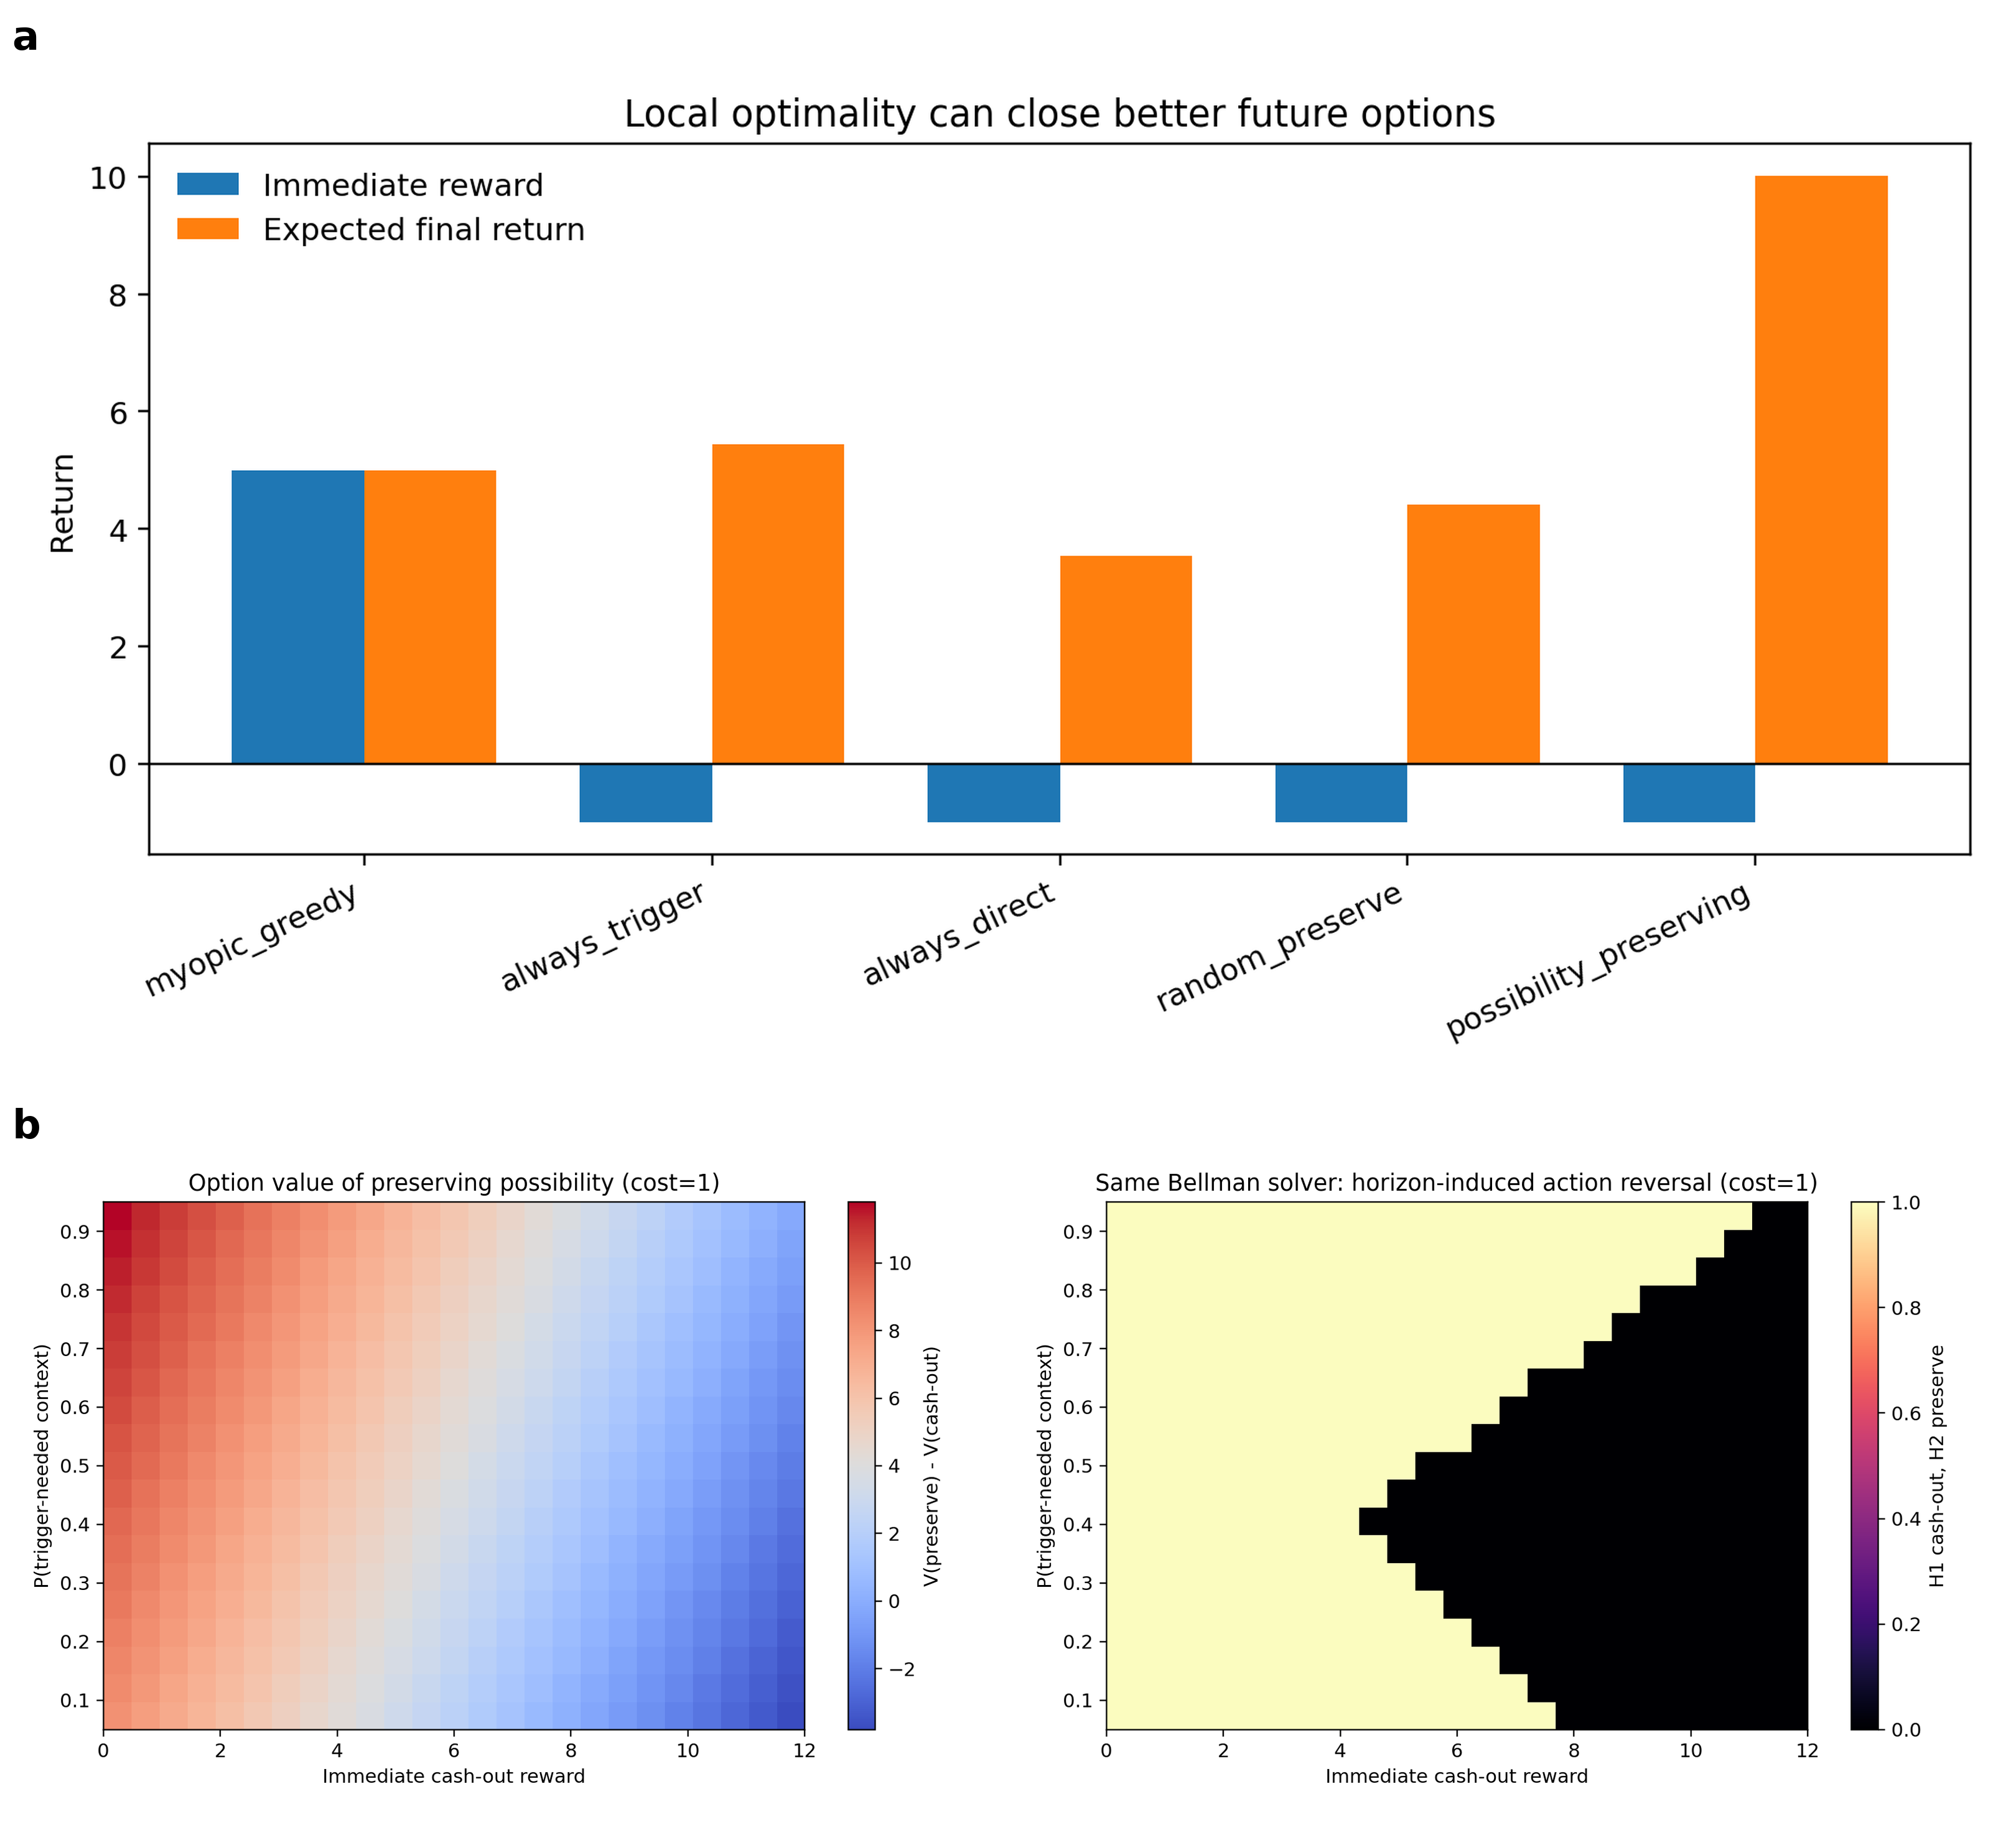
\includegraphics[width=0.92\linewidth]{ed_fig1.png}
  \caption{\textbf{Analytic core: option value of preserving
  possibility.}
  \textbf{a}, In the finite-horizon possibility tree, the myopically
  greedy policy maximizes immediate reward but closes the
  higher-return futures; the possibility-preserving policy pays a
  local cost and doubles the expected final return---local optimality
  can close better future options.
  \textbf{b}, The closed-form option-value boundary
  $V(\text{preserve}) - V(\text{cash-out})$ over context probability
  and immediate reward (left); the \emph{same} Bellman solver reverses
  its action as the horizon expands (right): possibility preservation
  is a rational consequence of long horizons, not an added
  preference. These closed-form structures are what the
  phase-boundary prediction of Fig.~6c instantiates empirically.}
  \label{fig:ed-analytic}
\end{figure}

\begin{figure}[p]
  \centering
  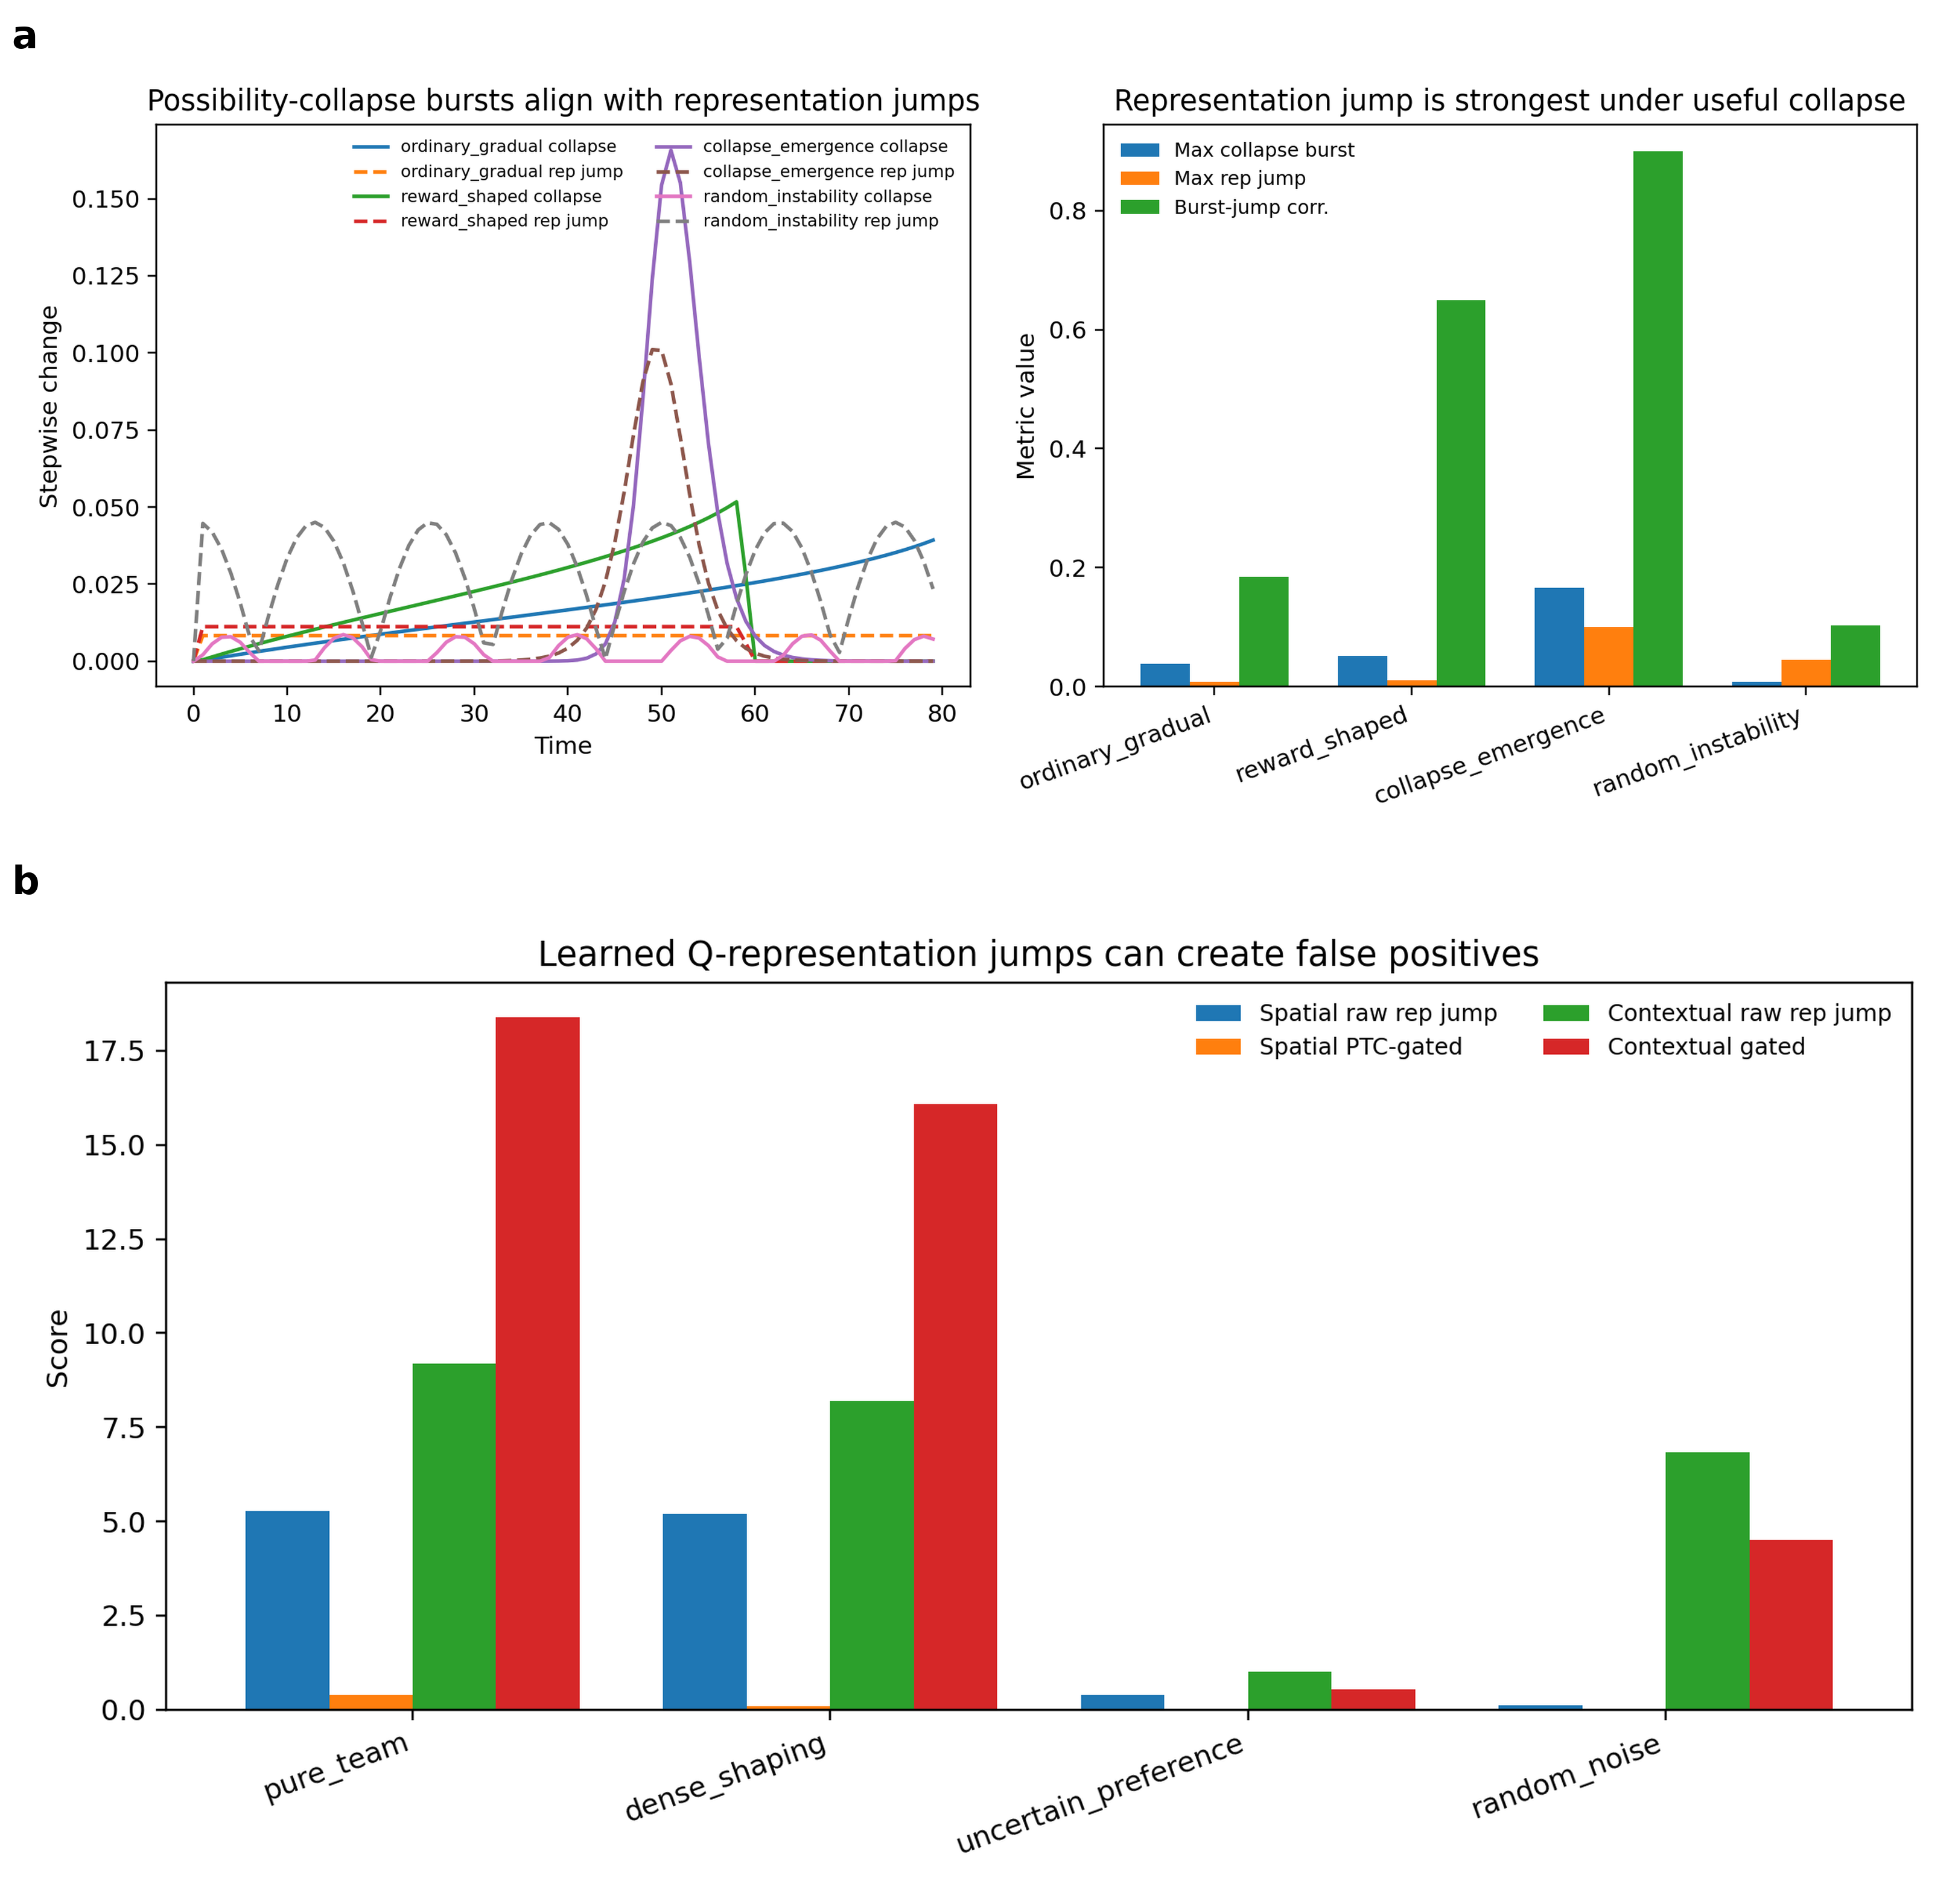
\includegraphics[width=0.92\linewidth]{ed_fig2.png}
  \caption{\textbf{Representation jumps are a bounded symptom, not a
  definition.}
  \textbf{a}, Training-time bridge across four regimes (collapse
  emergence, ordinary gradual, reward-shaped, random instability):
  collapse bursts and representation jumps co-occur in the emergence
  regime, and the Pinsker bound of Proposition~\ref{prop:pinsker}
  holds at every step of every trajectory.
  \textbf{b}, False-positive audit on learned representations:
  ordinary converged team reward and reward-shaped convergence produce
  jumps as large as (or larger than) true conditional emergence, and a
  noisy learner with the same acquired structure posts a
  $13.7\times$ larger jump---unsigned distance measures noise, not
  emergence.}
  \label{fig:ed-repjump}
\end{figure}

\begin{figure}[p]
  \centering
  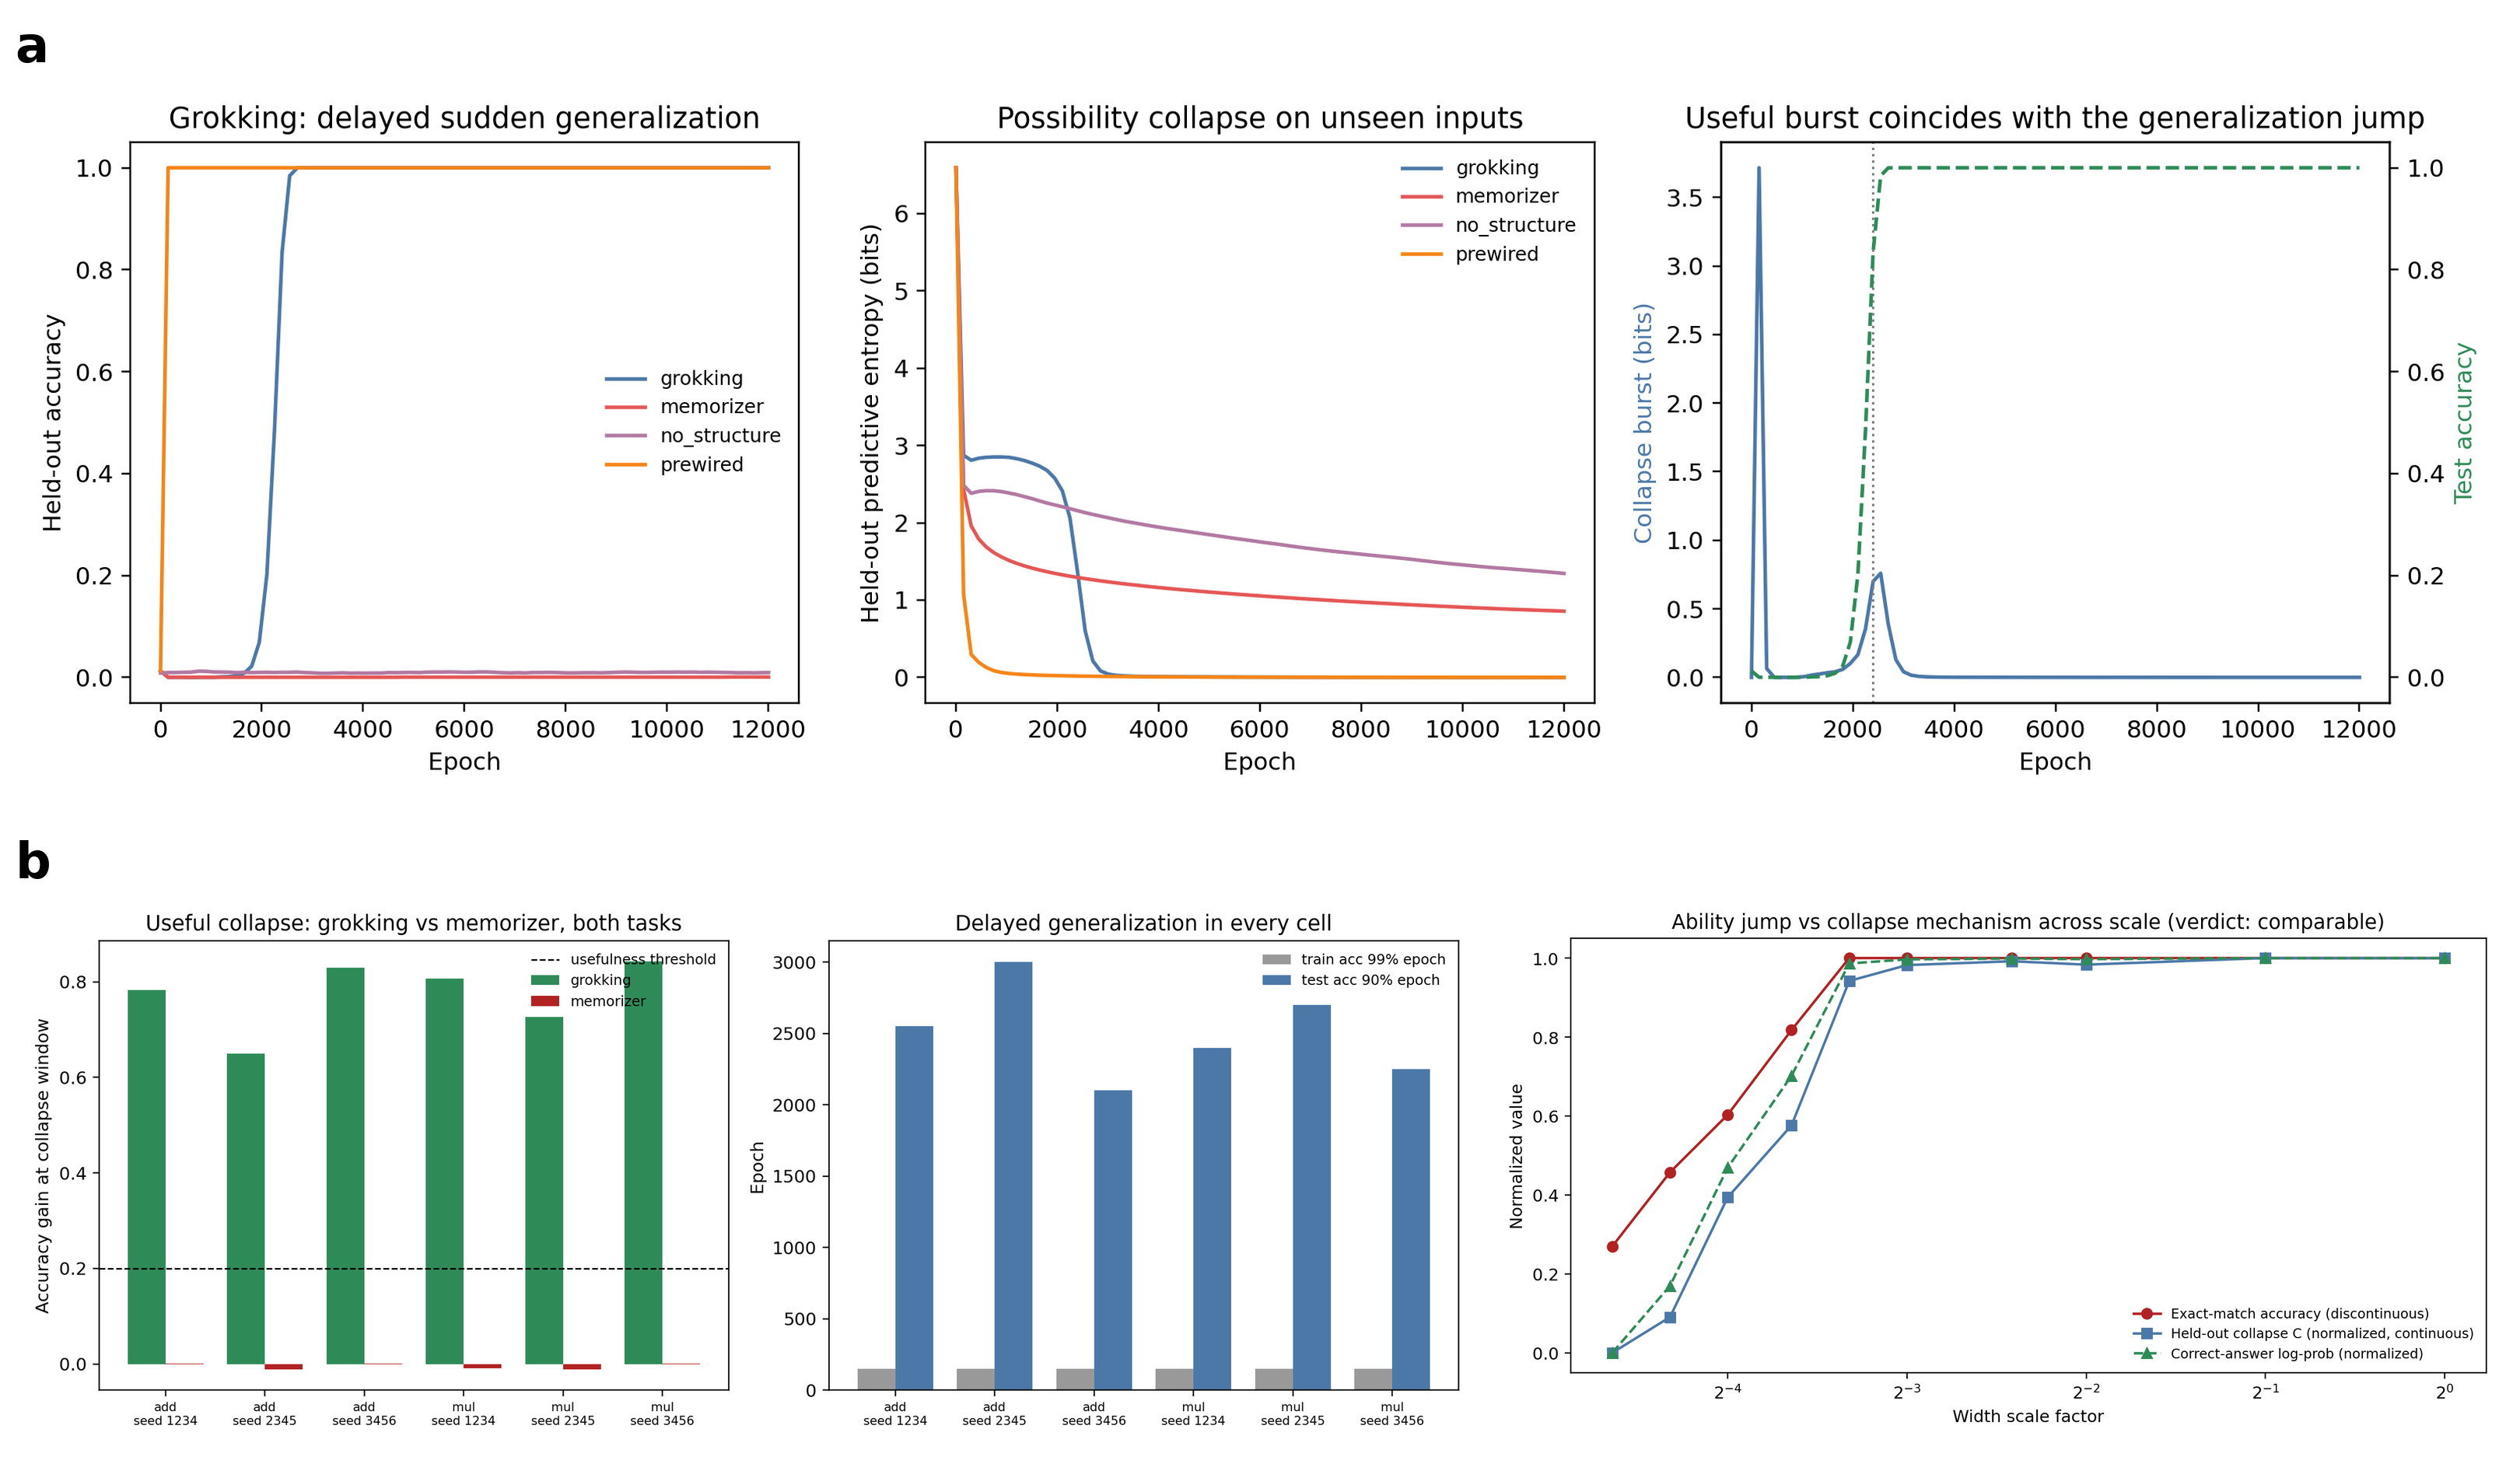
\includegraphics[width=\linewidth]{ed_fig3.png}
  \caption{\textbf{Grokking as useful possibility collapse.}
  \textbf{a}, Modular-addition grokking (MLP family): the grokking run
  passes all process-level components; the memorizer fails potential,
  burstiness and usefulness; the no-structure control fails
  burstiness and usefulness; the prewired run (evaluation distribution
  included in training) is excluded \emph{only} by endogeneity---the
  process-level analogue of reward shaping. The early memorization
  phase inside the grokking run itself is the sharpest internal
  control: held-out entropy drops $6.6 \to 2.8$ bits with zero
  accuracy gain, and the anchored window refuses to credit it.
  \textbf{b}, Generality sweep: 2 tasks $\times$ 3 seeds reproduce all
  verdicts (left); scale decomposition: the ability jump and the
  collapse transition land in the same scale region (right).}
  \label{fig:ed-grokking}
\end{figure}

\begin{figure}[p]
  \centering
  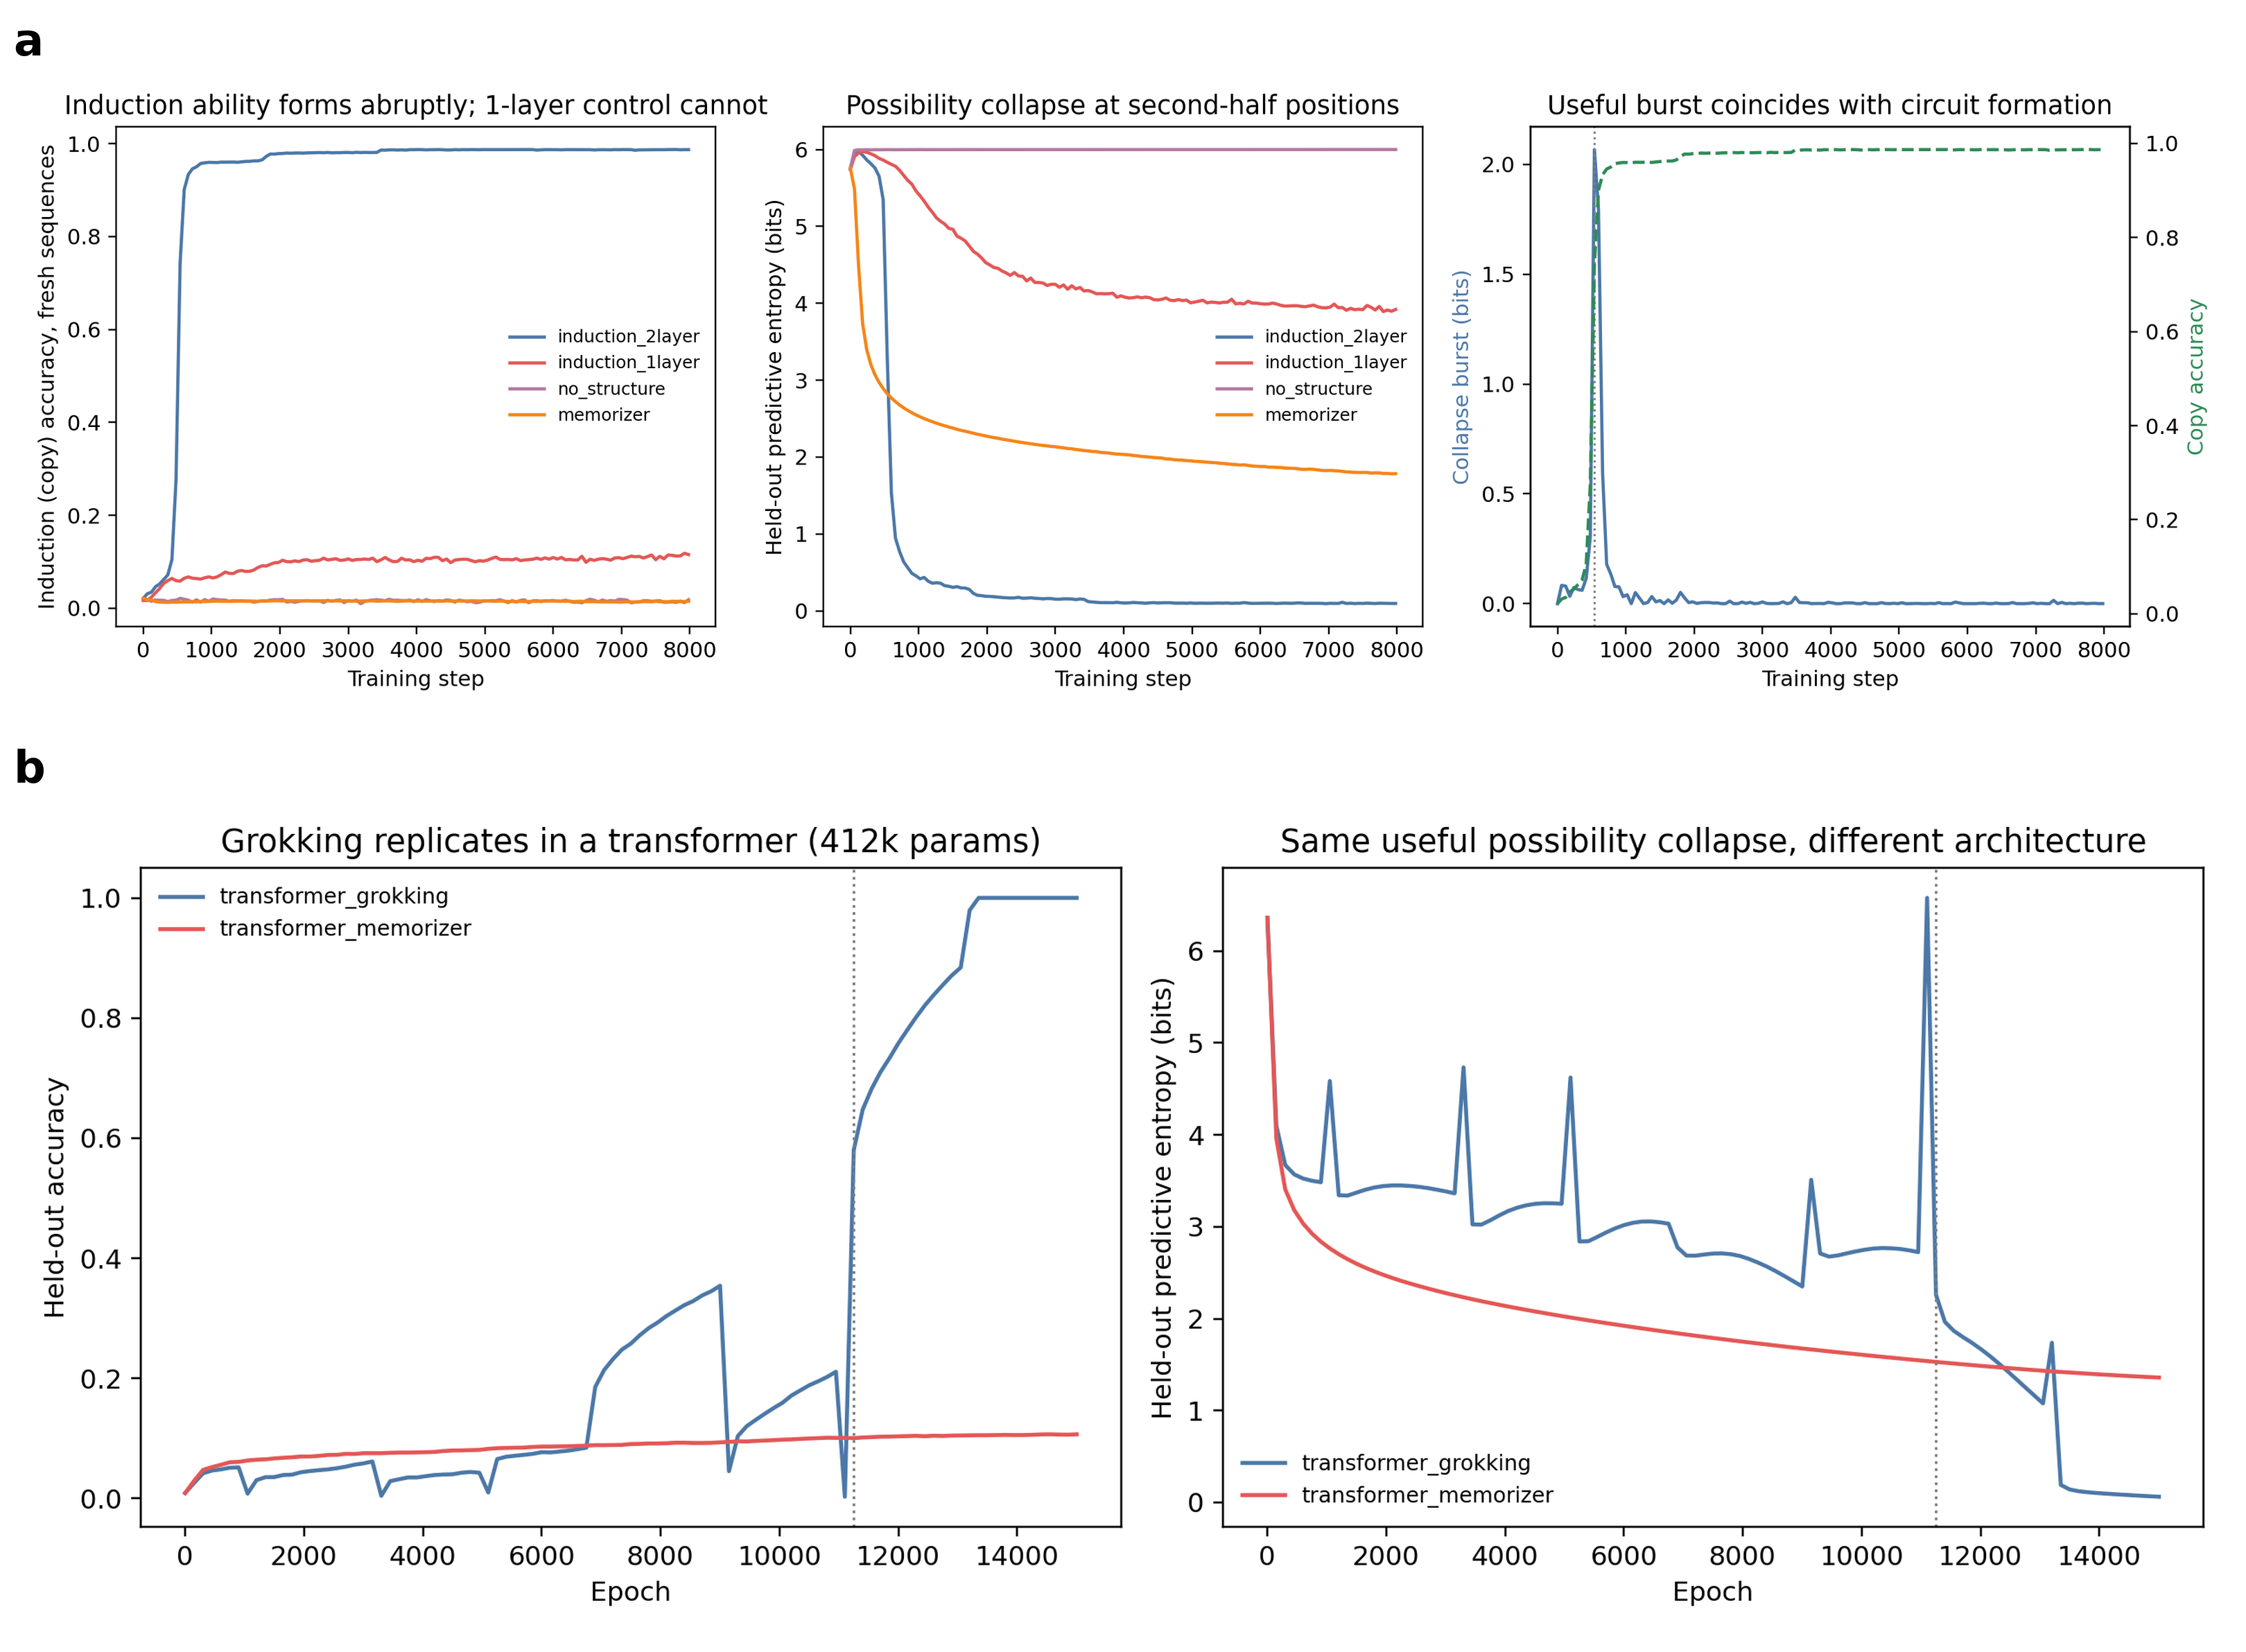
\includegraphics[width=\linewidth]{ed_fig4.png}
  \caption{\textbf{Externally discovered phase changes pass exactly
  when the architecture permits the circuit.}
  \textbf{a}, Induction-head formation (attention-only transformers on
  cyclic-repeat sequences): the two-layer model---which can implement
  the induction circuit---passes all process-proxy components (copy accuracy
  0.987); the one-layer model, provably unable to implement the
  circuit, fails usefulness (0.112); memorizer and no-structure
  controls fail as registered. 12/12 registered predictions on fresh
  seeds.
  \textbf{b}, Transformer replication of the grokking bridge: a 412k-
  parameter causal transformer grokks and passes; the same
  architecture without weight decay memorizes and fails usefulness.
  The process-level result spans MLP, causal-transformer, and
  attention-only families.}
  \label{fig:ed-induction}
\end{figure}

\begin{figure}[p]
  \centering
  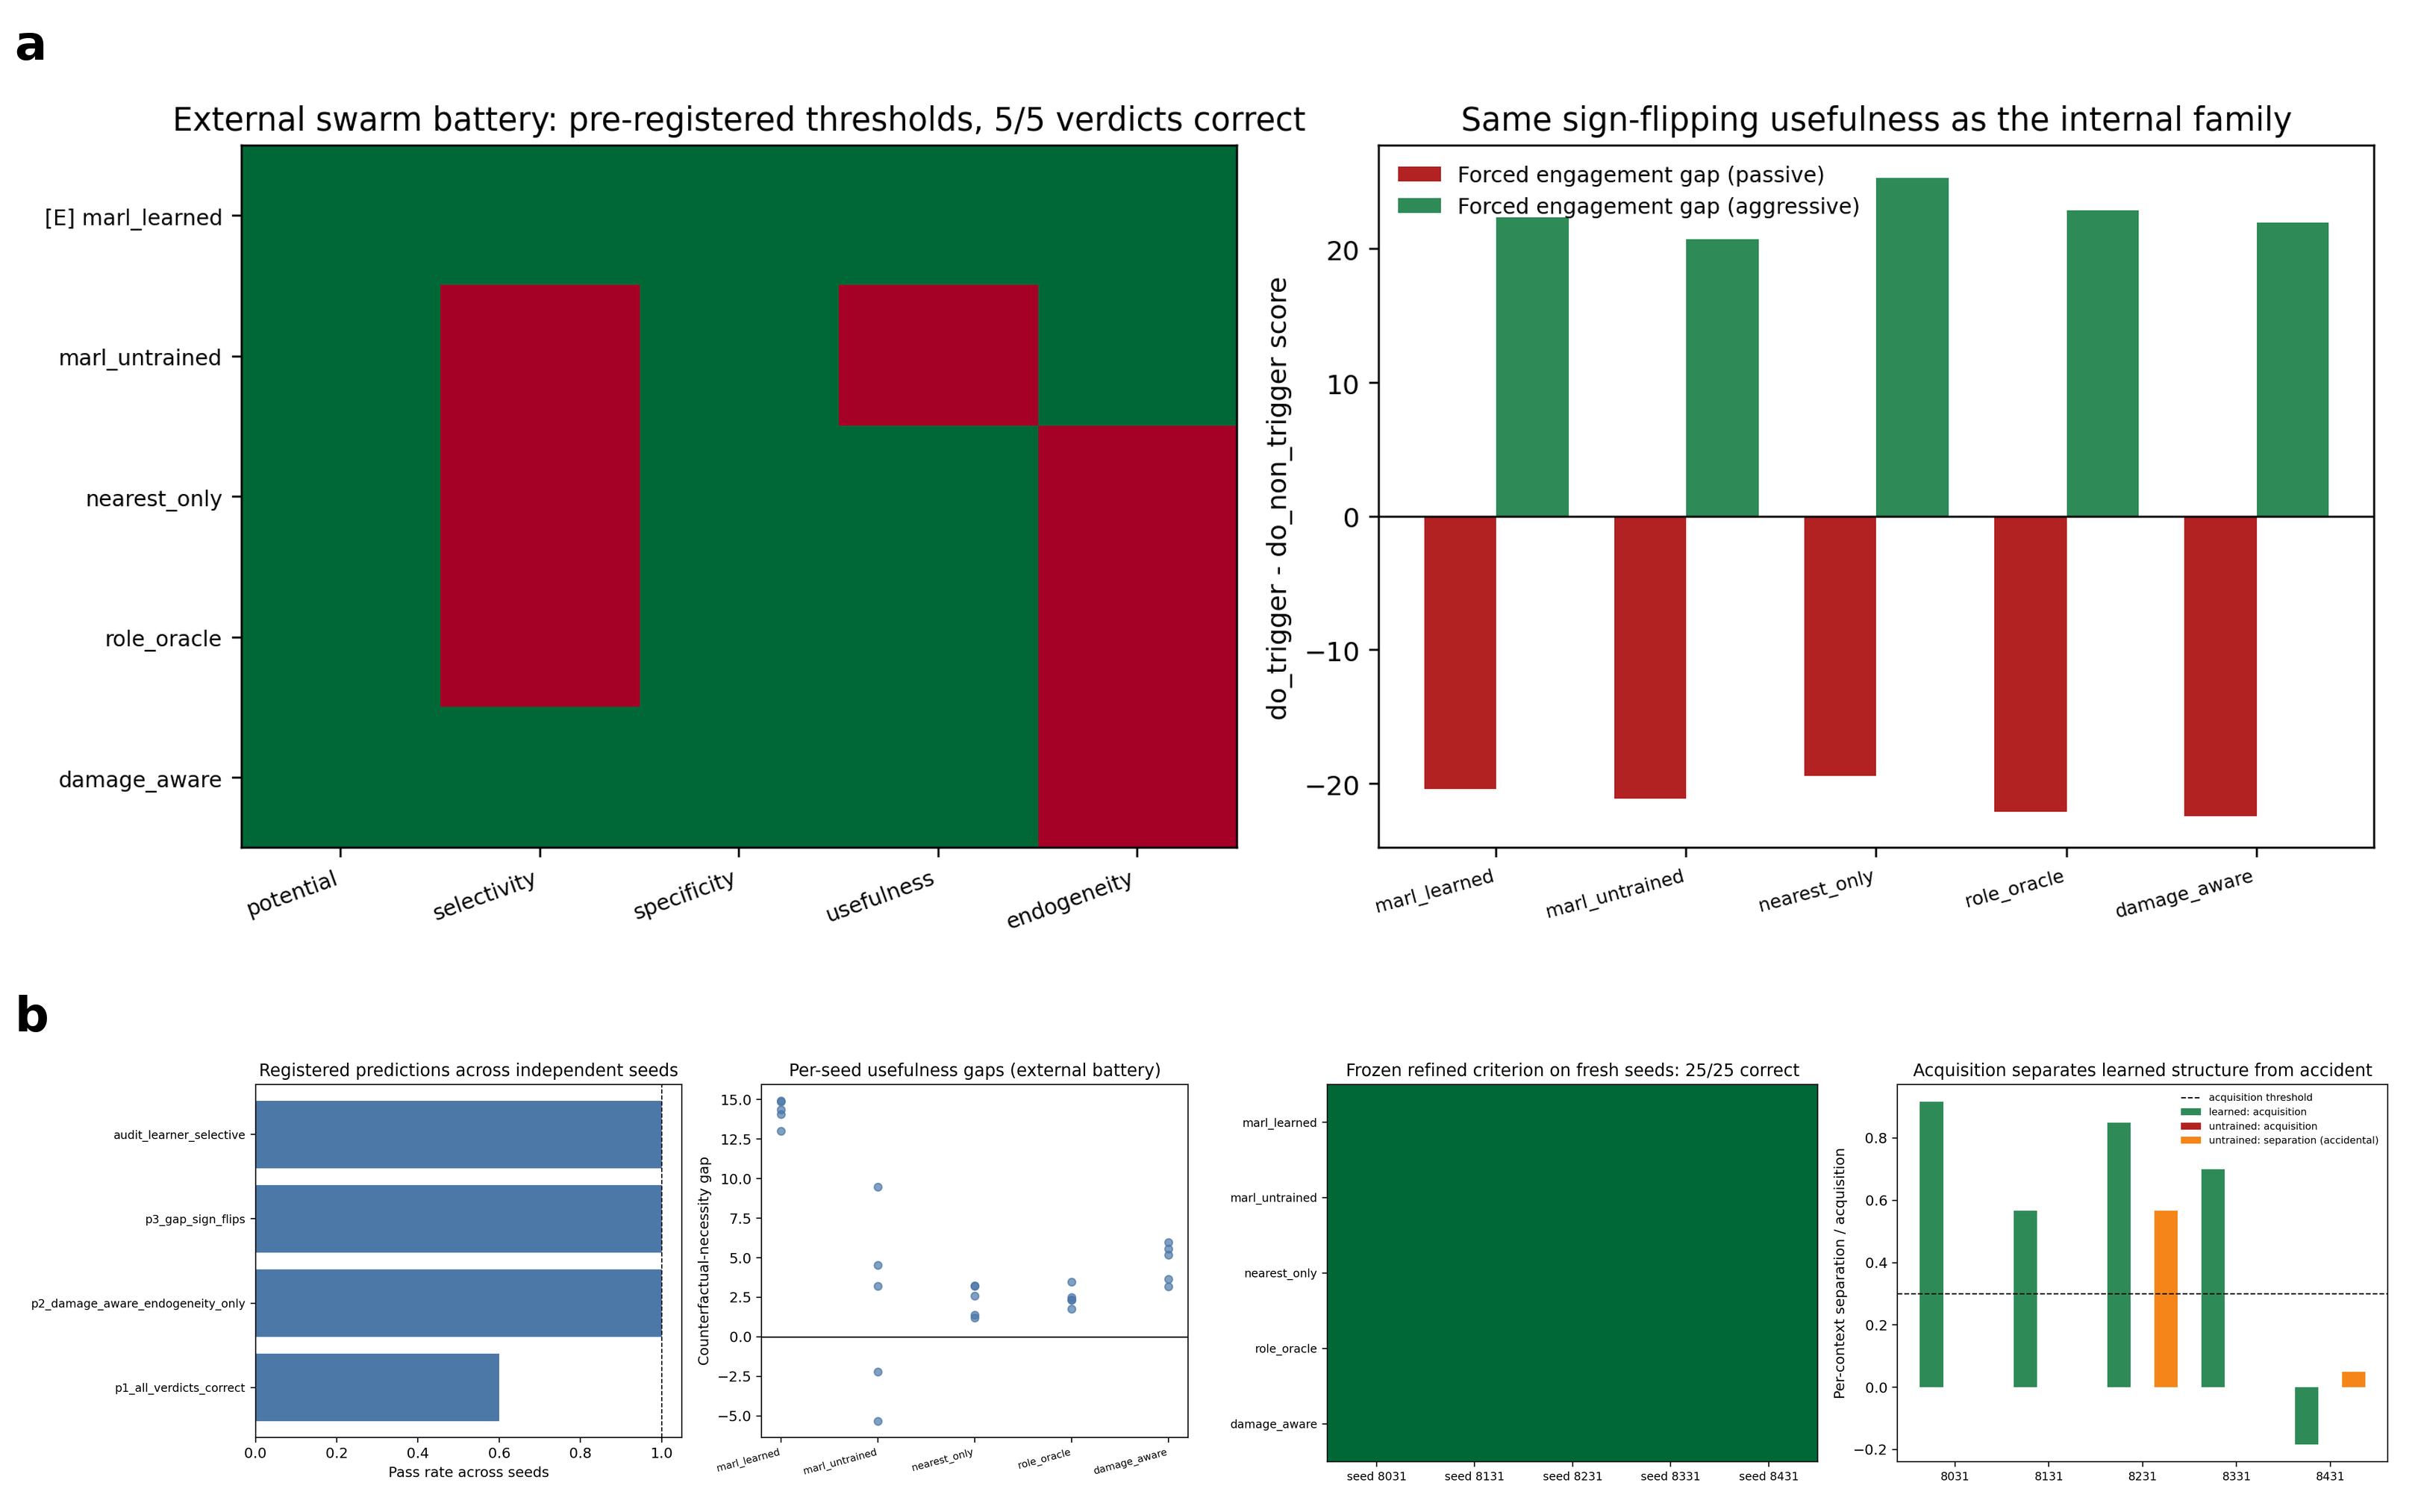
\includegraphics[width=\linewidth]{ed_fig5.png}
  \caption{\textbf{Prospectively frozen transfer to an external swarm
  benchmark.}
  \textbf{a}, Five controllers on a continuous decoy/targeting swarm
  environment sharing no state space, action space, or dynamics with
  the internal family, thresholds copied unchanged: only the learned
  controller (audited engagement rate 1.00 in the aggressive context,
  0.00 in the passive one) is accepted; the damage-aware
  controller---the external analogue of reward shaping---passes all
  four measured components and is excluded purely by endogeneity,
  pinning that component with an external counterexample.
  \textbf{b}, Multi-seed sweep with the registered failure (2/5 seeds
  accepted an untrained network on marginal tension; kept and
  reported) (left); the refined criterion (conditional selectivity,
  acquisition; frozen before new data) confirmed out-of-sample:
  25/25 external verdicts on five fresh seeds (right).}
  \label{fig:ed-swarm}
\end{figure}

\begin{figure}[p]
  \centering
  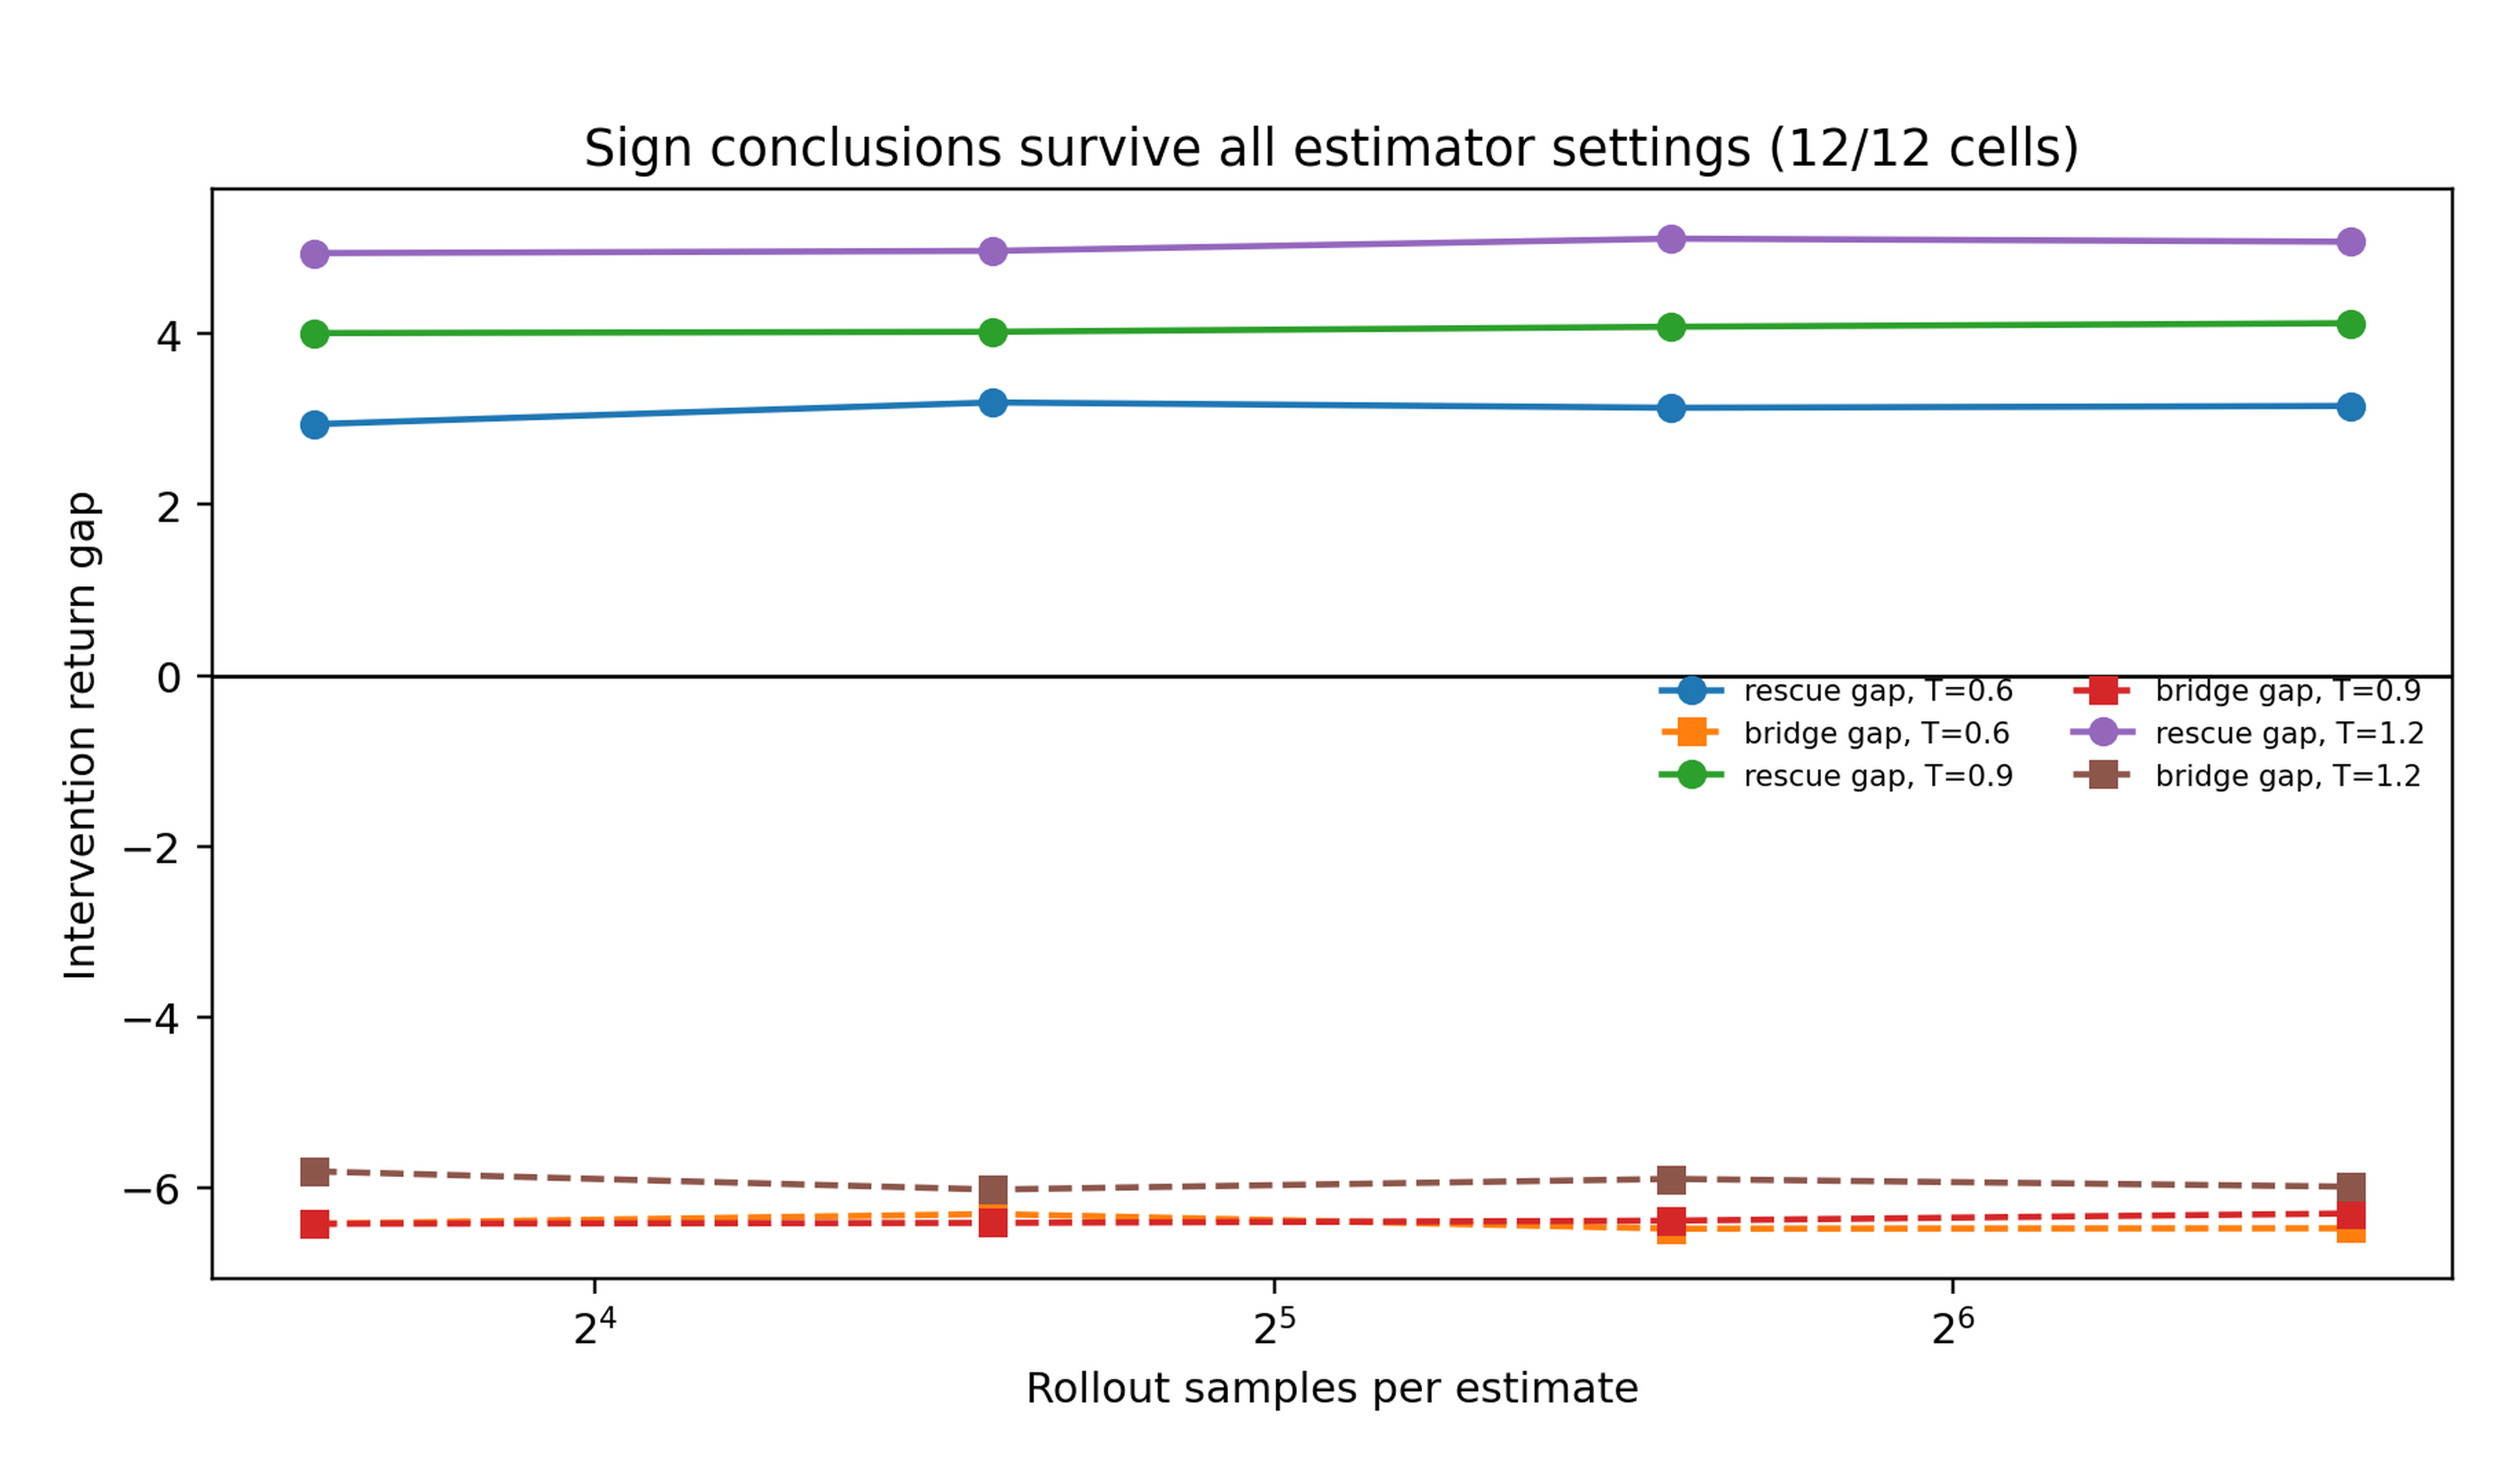
\includegraphics[width=0.9\linewidth]{ed_fig6.png}
  \caption{\textbf{Estimator robustness.} All qualitative conclusions
  of the within-episode probes (do-contrast signs, potential ordering)
  are unchanged across rollout counts $n \in \{12..96\}$ and probe
  temperatures (12-cell grid). Together with the 12-cell chess grid
  (Fig.~5b) and the LBF probe-temperature grid (Methods), this
  documents where the framework is estimator-robust and where its one
  declared observer-dependence lies: the \emph{absolute} scale of the
  potential component.}
  \label{fig:ed-robust}
\end{figure}

\begin{figure}[p]
  \centering
  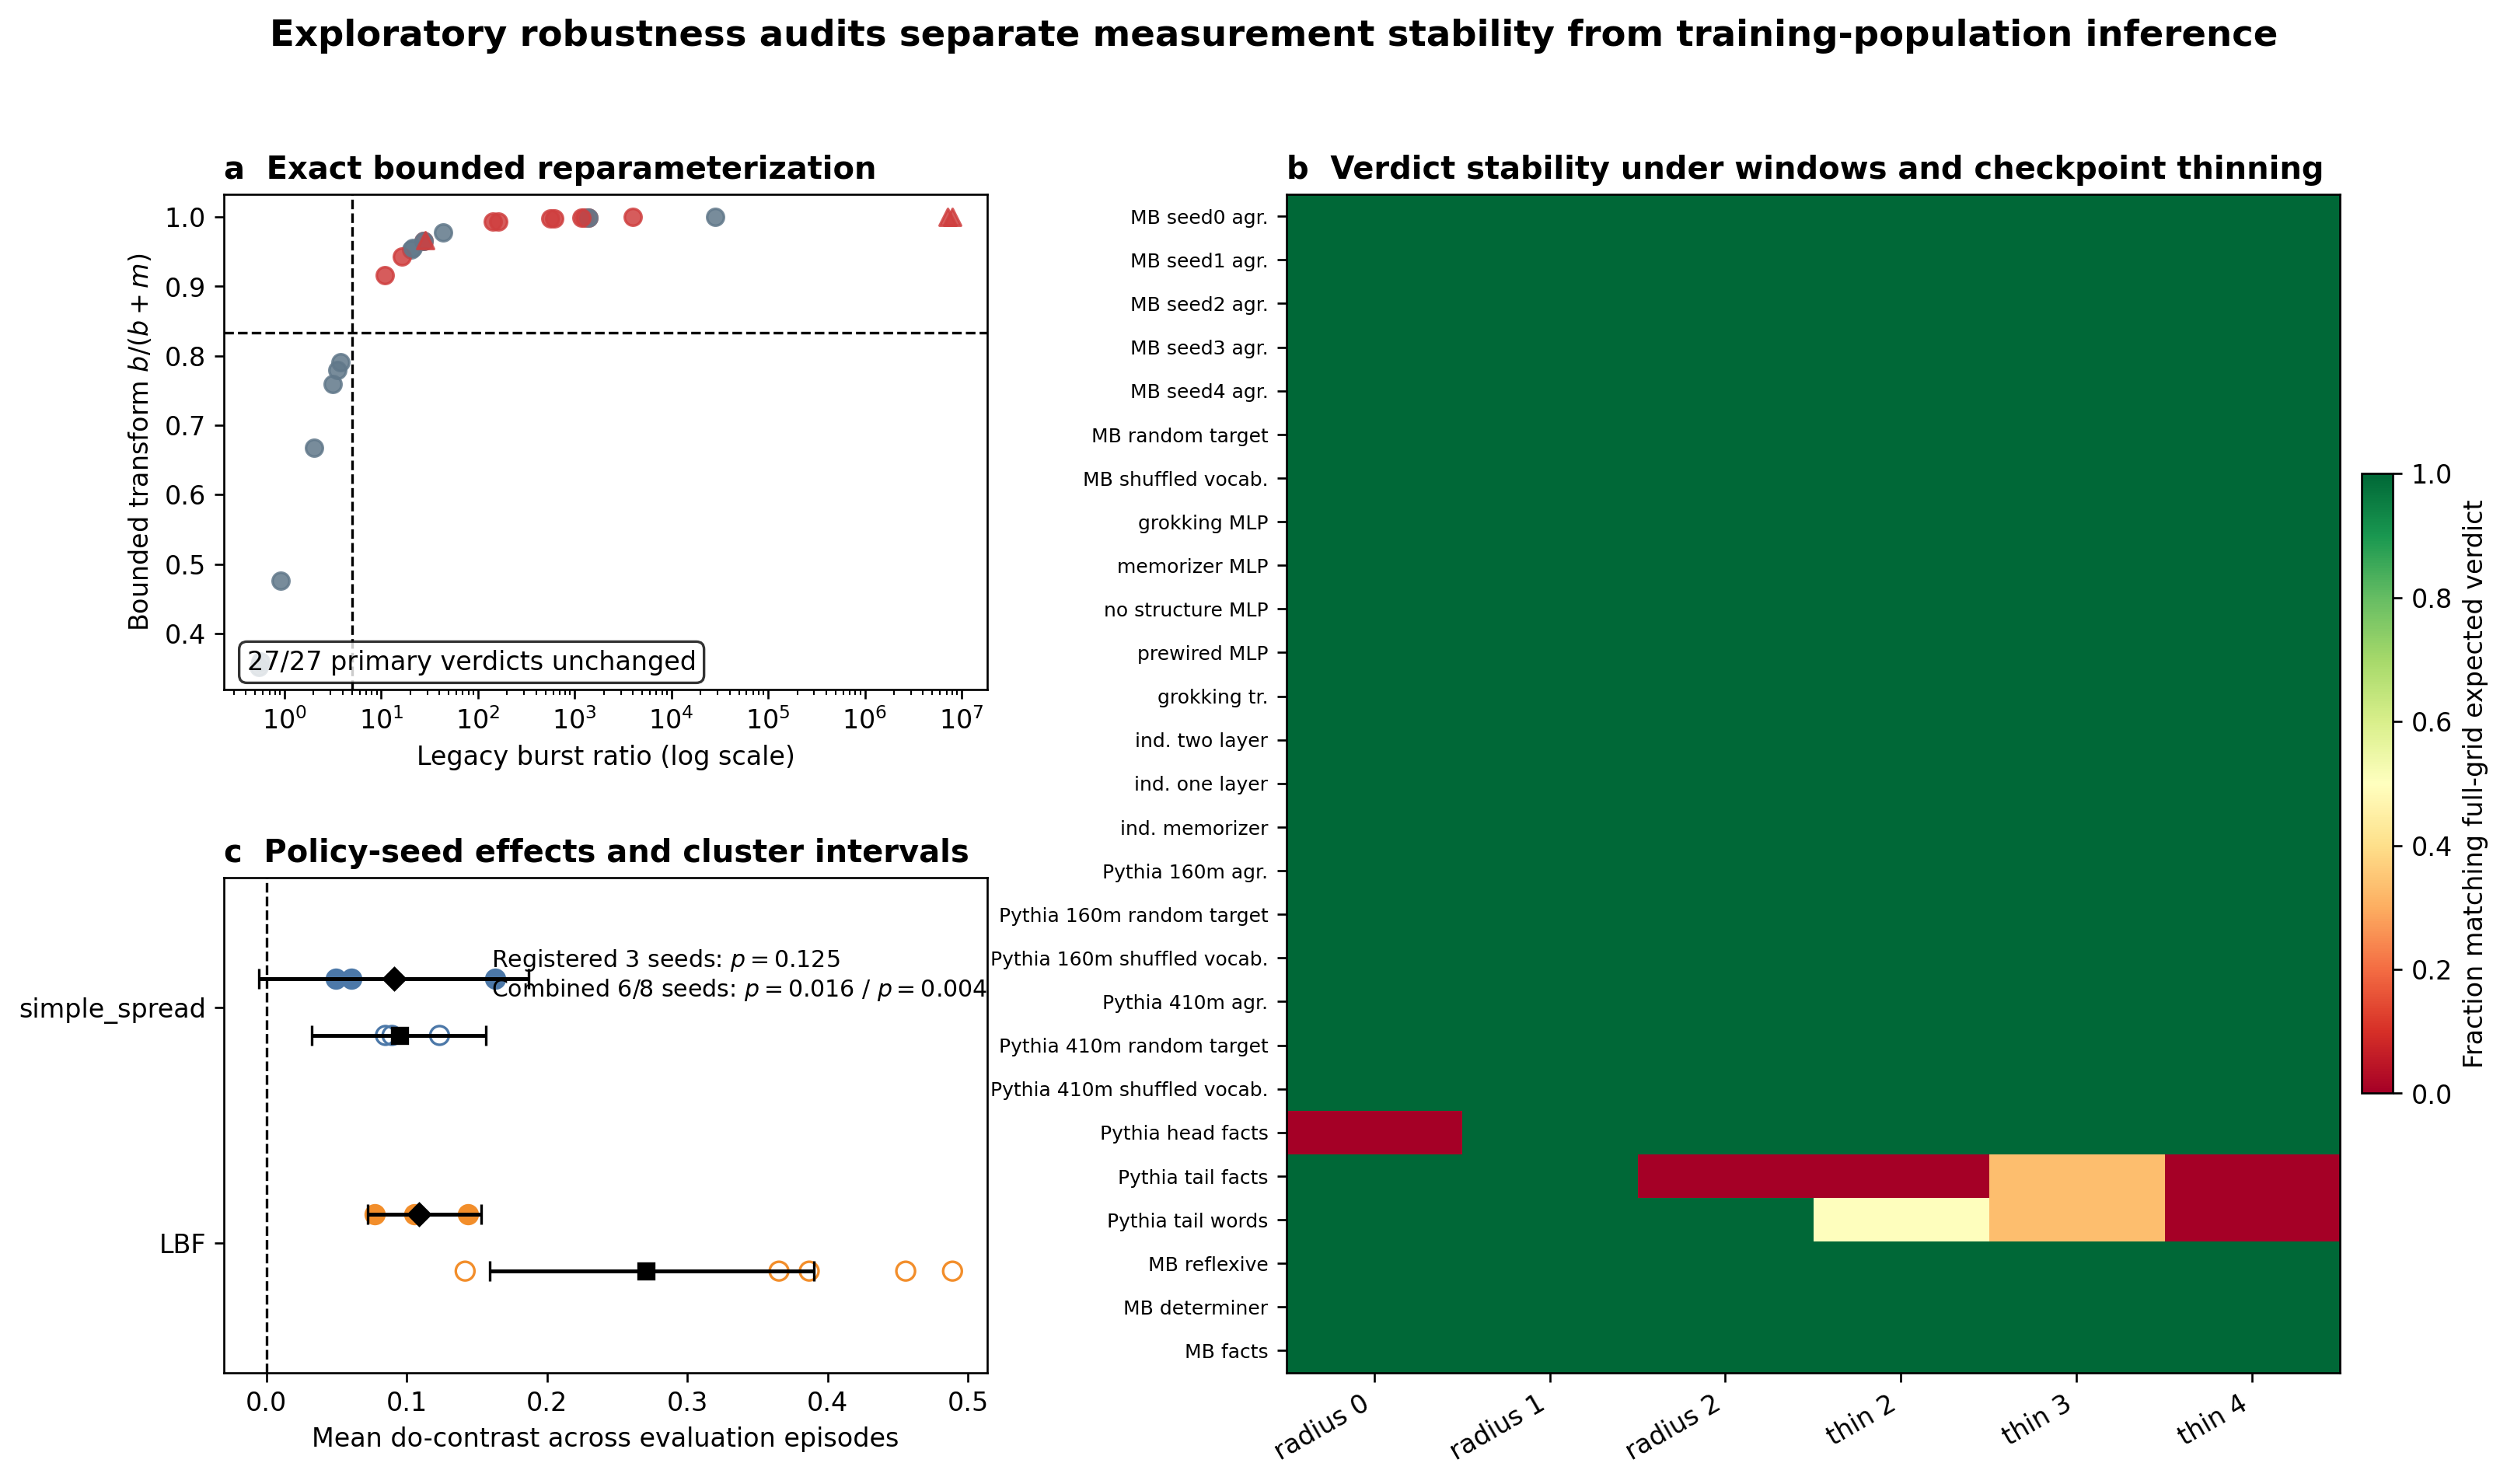
\includegraphics[width=\linewidth]{ed_fig7_robustness_hierarchy.png}
  \caption{\textbf{Exploratory process-grid robustness and seed-aware
  MARL inference.}
  \textbf{a}, The bounded burst statistic is a monotone
  reparameterization of the frozen ratio; its threshold $5/6$ is
  exactly the legacy ratio threshold 5, and 27/27 primary verdicts are
  unchanged.
  \textbf{b}, Verdict agreement under window radii 0--2 and checkpoint
  thinning factors 2--4. Full-grid agreement is perfect; 228/243
  thinning cells agree, with disagreements concentrated in two Pythia
  tail controls.
  \textbf{c}, Per-policy-seed mean do-gaps for the three registered
  seeds (filled circles; diamonds/lines give their two-stage
  seed--episode bootstrap intervals) and for the post-hoc seed
  extension (open circles; squares/lines give the combined-seed
  intervals). With three seeds the exact positive-seed sign test is
  $p=0.125$ in either domain and the simple\_spread mean interval
  crosses zero; the extension (three more simple\_spread and five more
  LBF policies, all positive) tightens these to $p=0.016$ and
  $p=0.004$ with positive combined mean intervals (Methods). All
  panels are post-hoc robustness analyses and are not counted as
  prospectively registered confirmations.}
  \label{fig:ed-newrobust}
\end{figure}

\begin{figure}[p]
  \centering
  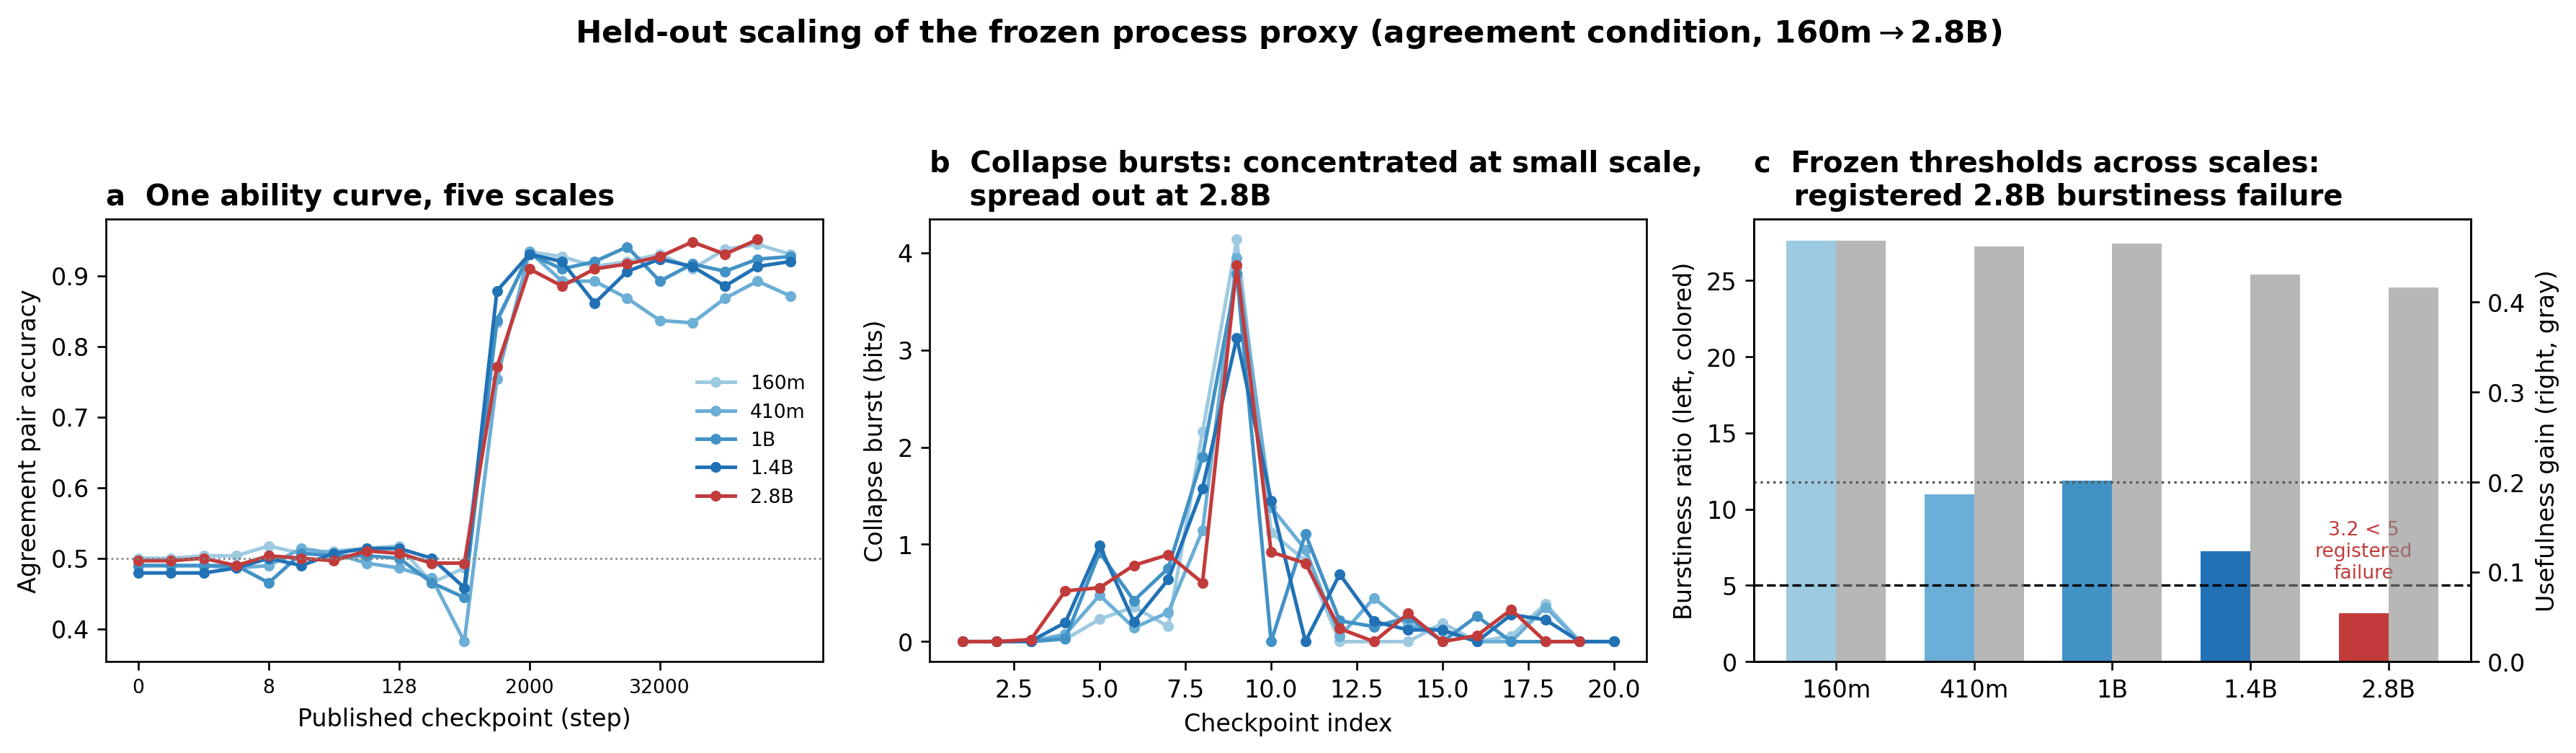
\includegraphics[width=\linewidth]{ed_fig9_pythia_scaling.png}
  \caption{\textbf{Held-out scaling of the frozen process proxy
  (Pythia agreement condition, 160m--2.8B).}
  \textbf{a}, The same templated subject--verb-agreement battery under
  identical frozen thresholds at five public scales; every scale
  crosses from chance to $>0.85$ within the same checkpoint region.
  \textbf{b}, Collapse bursts along the published checkpoint grid. At
  160m--1.4B one dominant burst precedes the ability jump; at 2.8B the
  same total collapse is spread over several early intervals.
  \textbf{c}, Component values against the frozen cutoffs (dashed:
  burstiness 5; dotted: usefulness 0.2). Usefulness passes at every
  scale; burstiness declines monotonically with scale and fails
  registered prediction S1 at 2.8B ($3.2<5$), kept as a registered
  failure. Under every $2$--$4\times$ checkpoint thinning the 2.8B
  verdict flips back to accept (registered S7 failure, $80.2\%<90\%$
  agreement), identifying the failure as grid-relative: larger models
  acquire the ability faster and more diffusely than the published
  log-spaced grid can resolve.}
  \label{fig:ed-scaling}
\end{figure}

\begin{figure}[p]
  \centering
  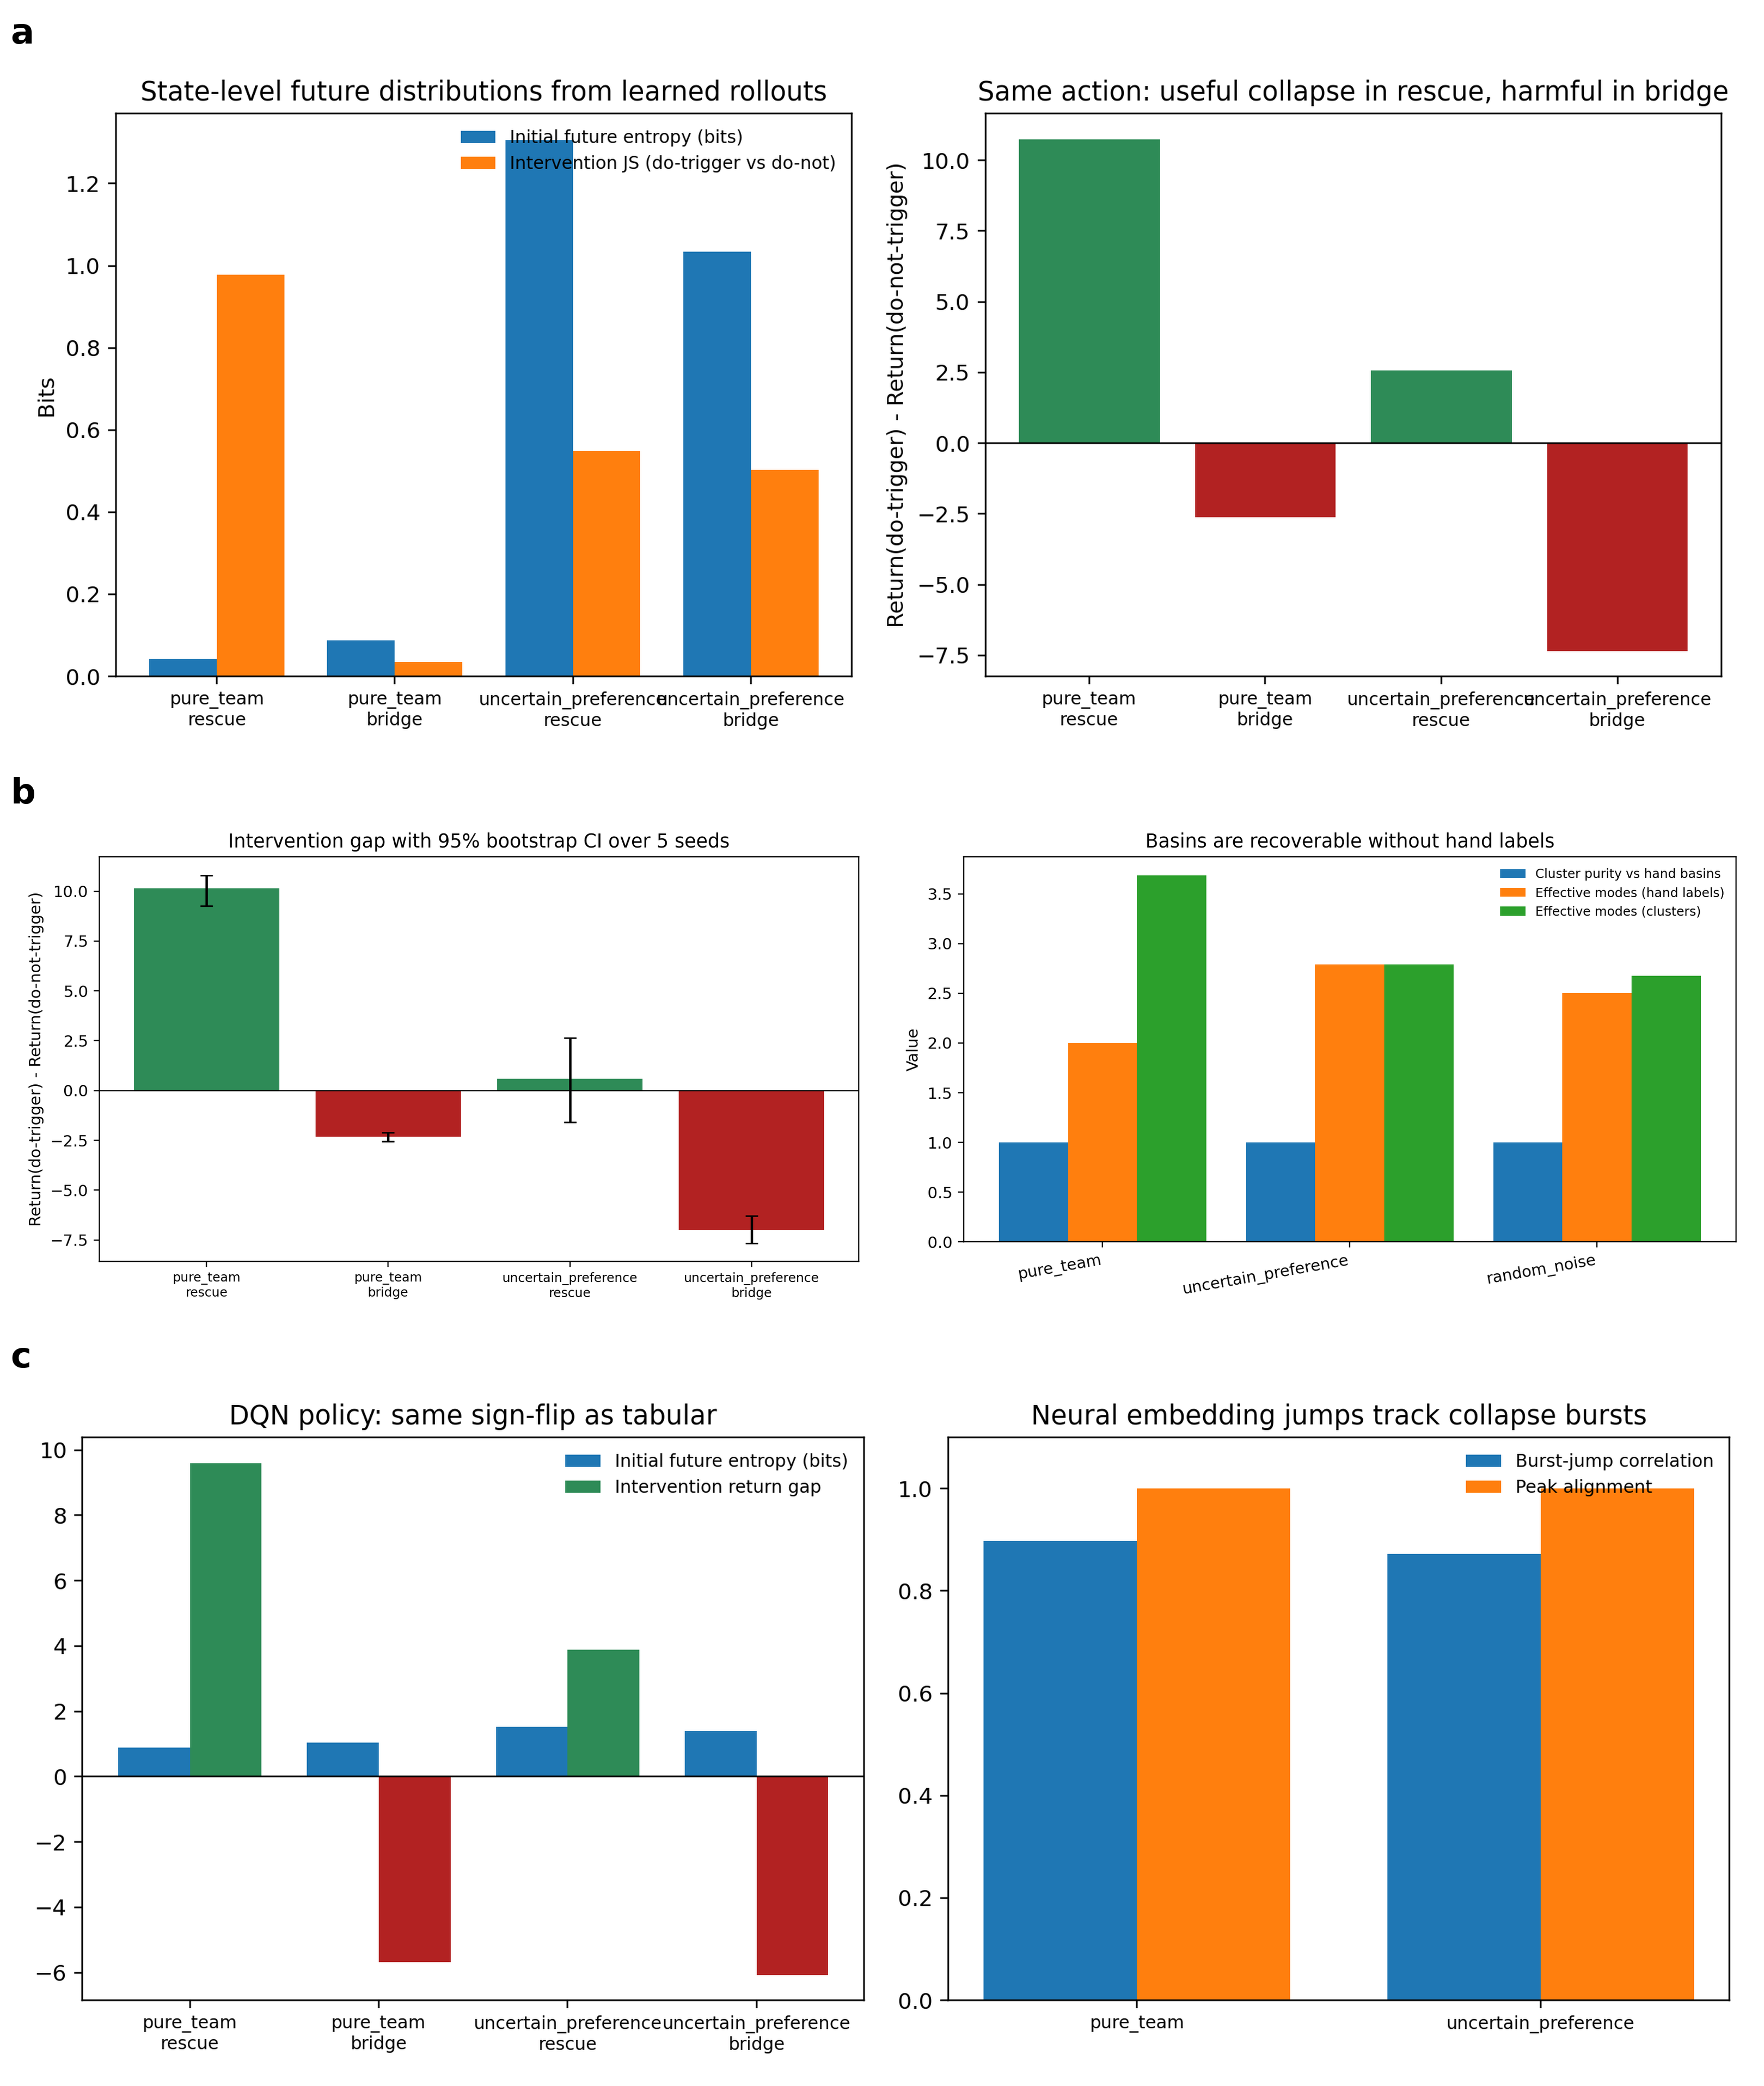
\includegraphics[width=\linewidth]{ed_fig10_mechanism.png}
  \caption{\textbf{The mechanism within single episodes.}
  \textbf{a}, State-level future distributions from learned rollouts:
  initial future entropy and intervention JS (left); the same action
  produces a useful collapse in the rescue context and a harmful one
  in the bridge context---the sign flip no unsigned signature carries
  (right).
  \textbf{b}, Intervention gaps with bootstrap 95\% CIs over five
  seeds (left); basins are recoverable without hand labels: label-free
  clustering matches hand basins with purity $1.00$ in the internal
  regimes and preserves effective-mode counts in the key
  uncertain-preference condition (right; pure-team loss episodes split
  more finely).
  \textbf{c}, Neural (DQN) replication shows the same sign structure
  (left), and neural embedding jumps track collapse bursts
  (correlation $0.87$--$0.90$, peak alignment $1.0$; right)---the
  representation jump as a downstream symptom, as
  Proposition~\ref{prop:pinsker} requires.}
  \label{fig:ed-mechanism}
\end{figure}

\begin{figure}[p]
  \centering
  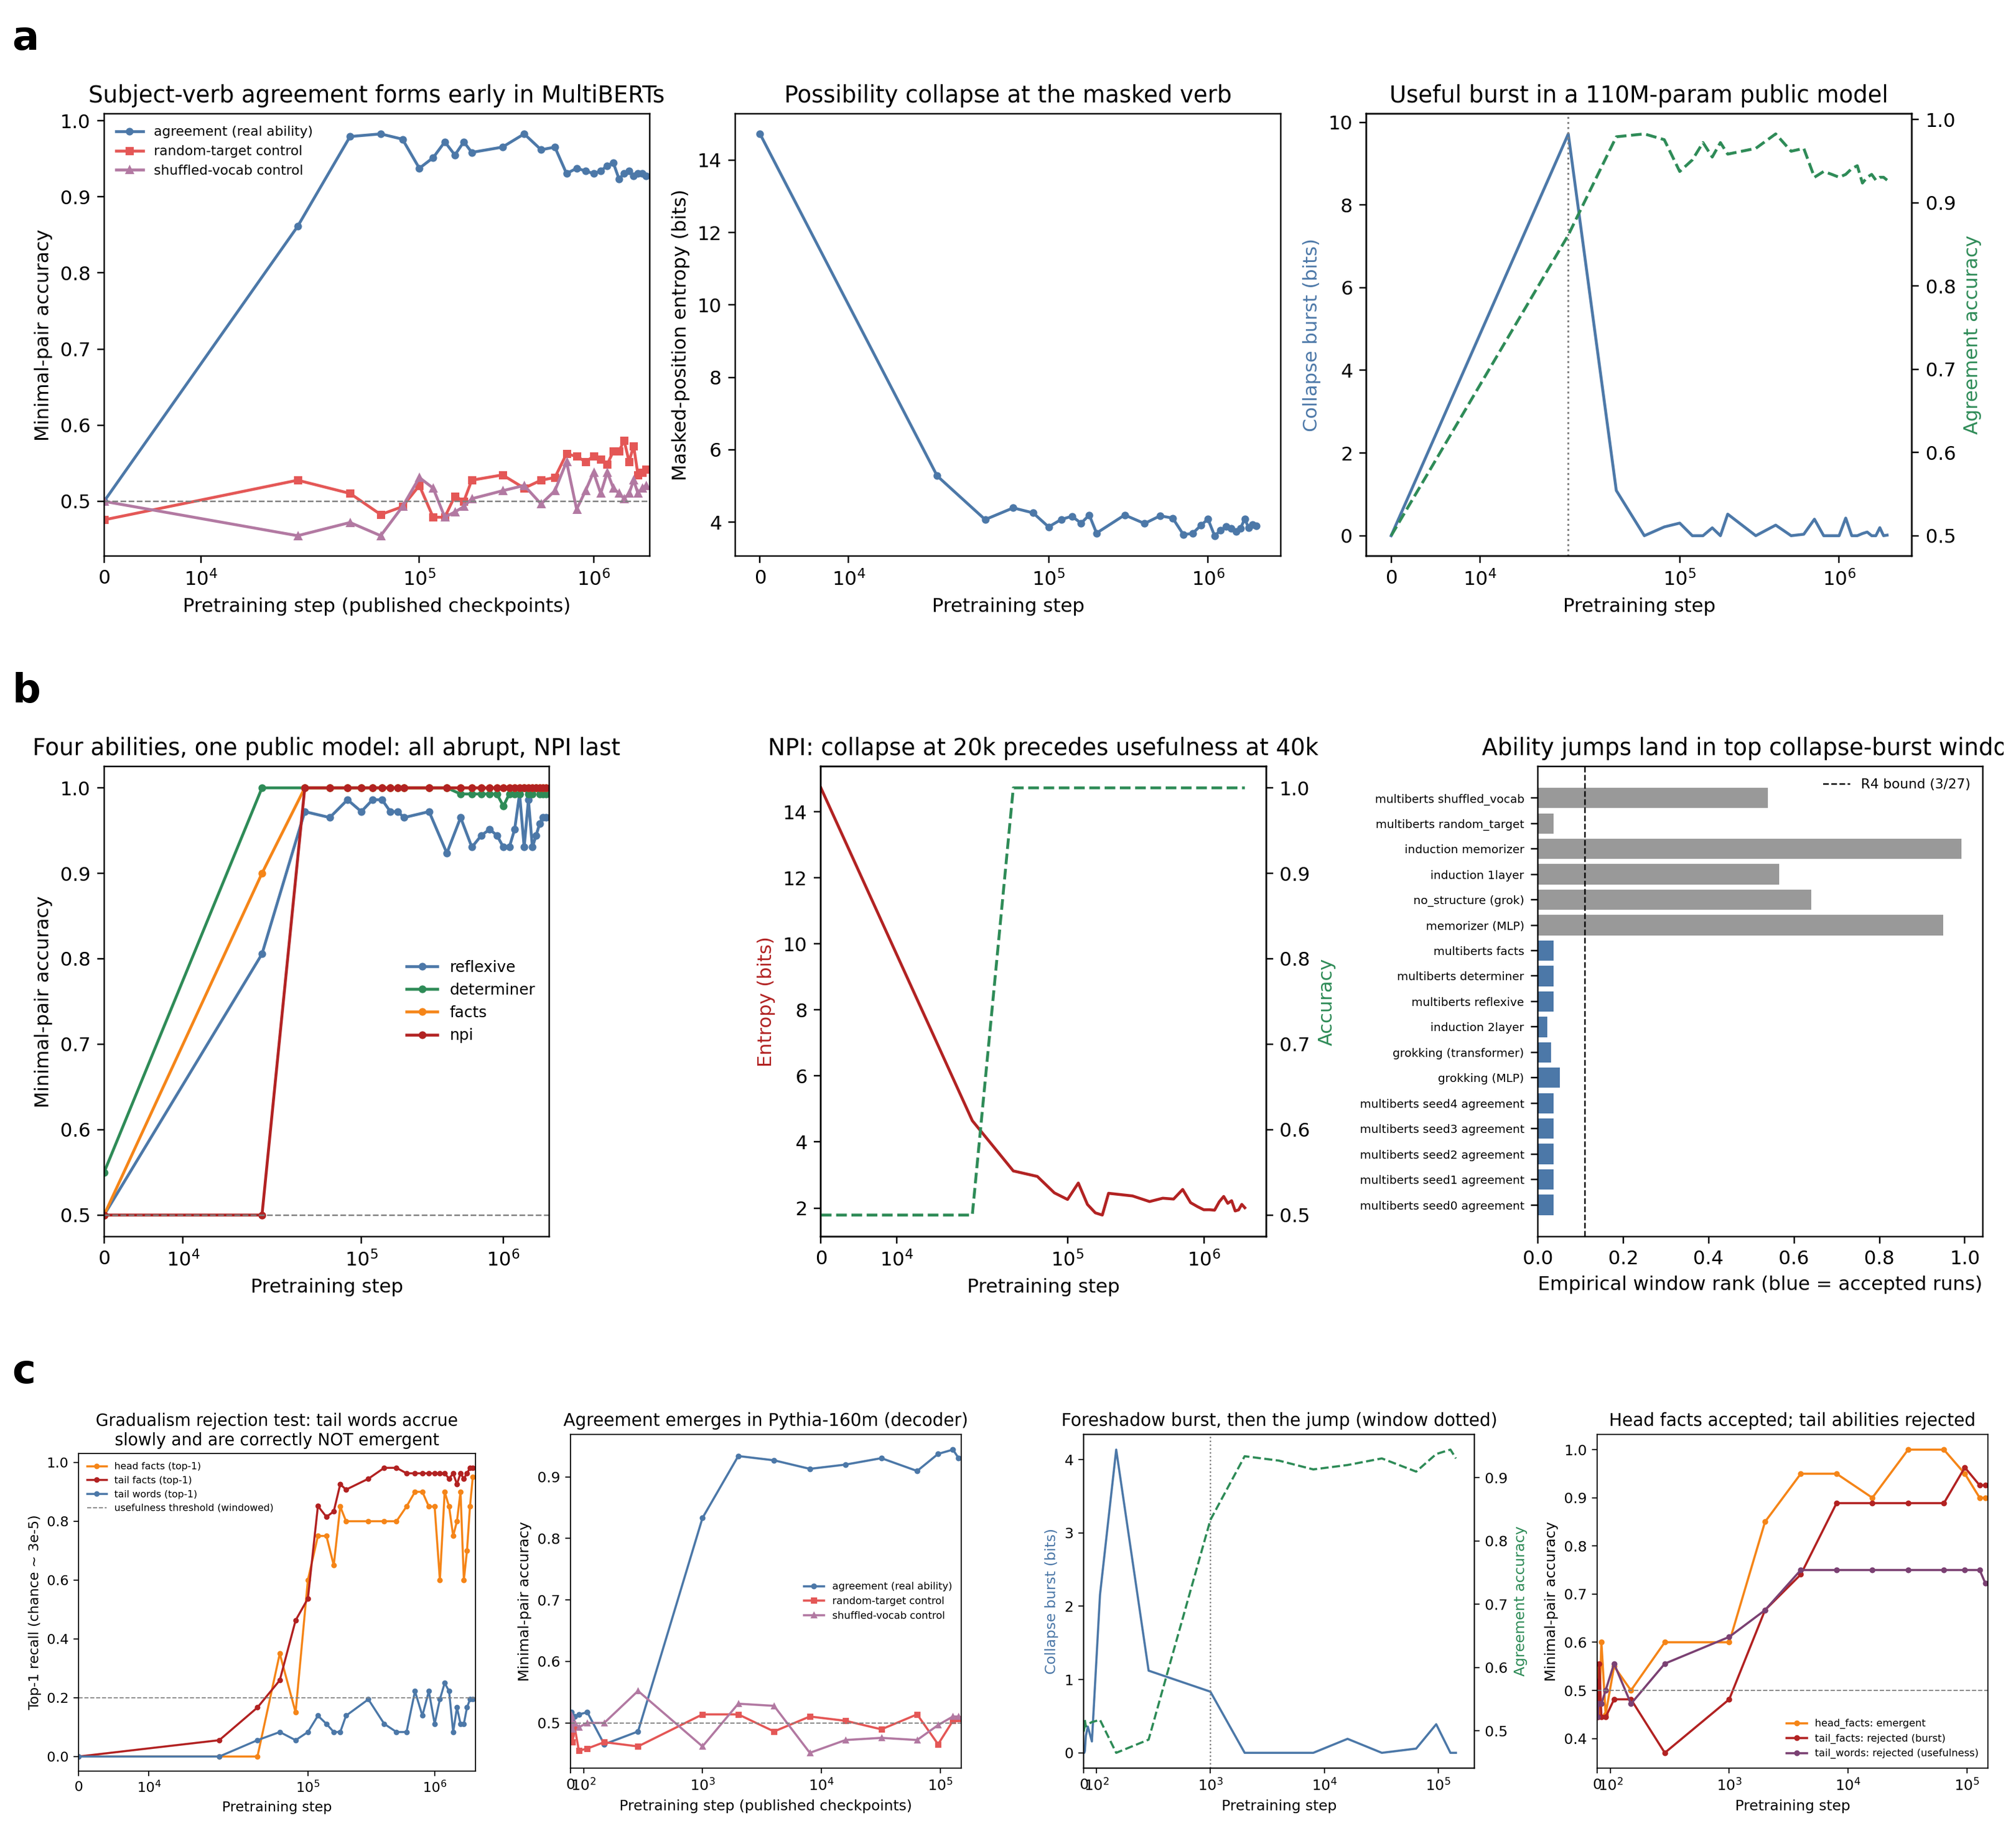
\includegraphics[width=\linewidth]{ed_fig11_public.png}
  \caption{\textbf{Training-time acquisition in public checkpoint series
  (no authorial control over training; observer protocol author-defined).}
  \textbf{a}, MultiBERTs: subject--verb agreement accuracy jumps
  $0.50 \to 0.98$ while random-target and shuffled-vocabulary controls
  stay at chance (left); the masked-verb possibility space collapses
  from $14.7$ bits (middle); the collapse burst coincides with the
  ability jump (right; agreement accepted 5/5 seeds and paired controls
  rejected, not 15 independent trials).
  \textbf{b}, Five-ability battery on the published checkpoint grid,
  NPI last (left); the NPI case shows collapse at 20k
  \emph{preceding} usefulness at 40k (middle); a permutation test puts
  every accepted run's jump in a top collapse-burst window (right;
  descriptive per-run empirical ranks, not an omnibus significance test).
  \textbf{c}, The rejection side. Left: MultiBERTs tail-gradualism
  test---tail words accrue slowly and are correctly \emph{not}
  emergent. Right three panels: Pythia decoder series---agreement
  emerges with both controls at chance; the foreshadow burst precedes
  the jump (dotted anchored window); head facts are accepted while
  \emph{both} frequency-tail families are rejected, through two
  different components. Verified at two scales (160m, 410m).}
  \label{fig:ed-public}
\end{figure}

\begin{figure}[p]
  \centering
  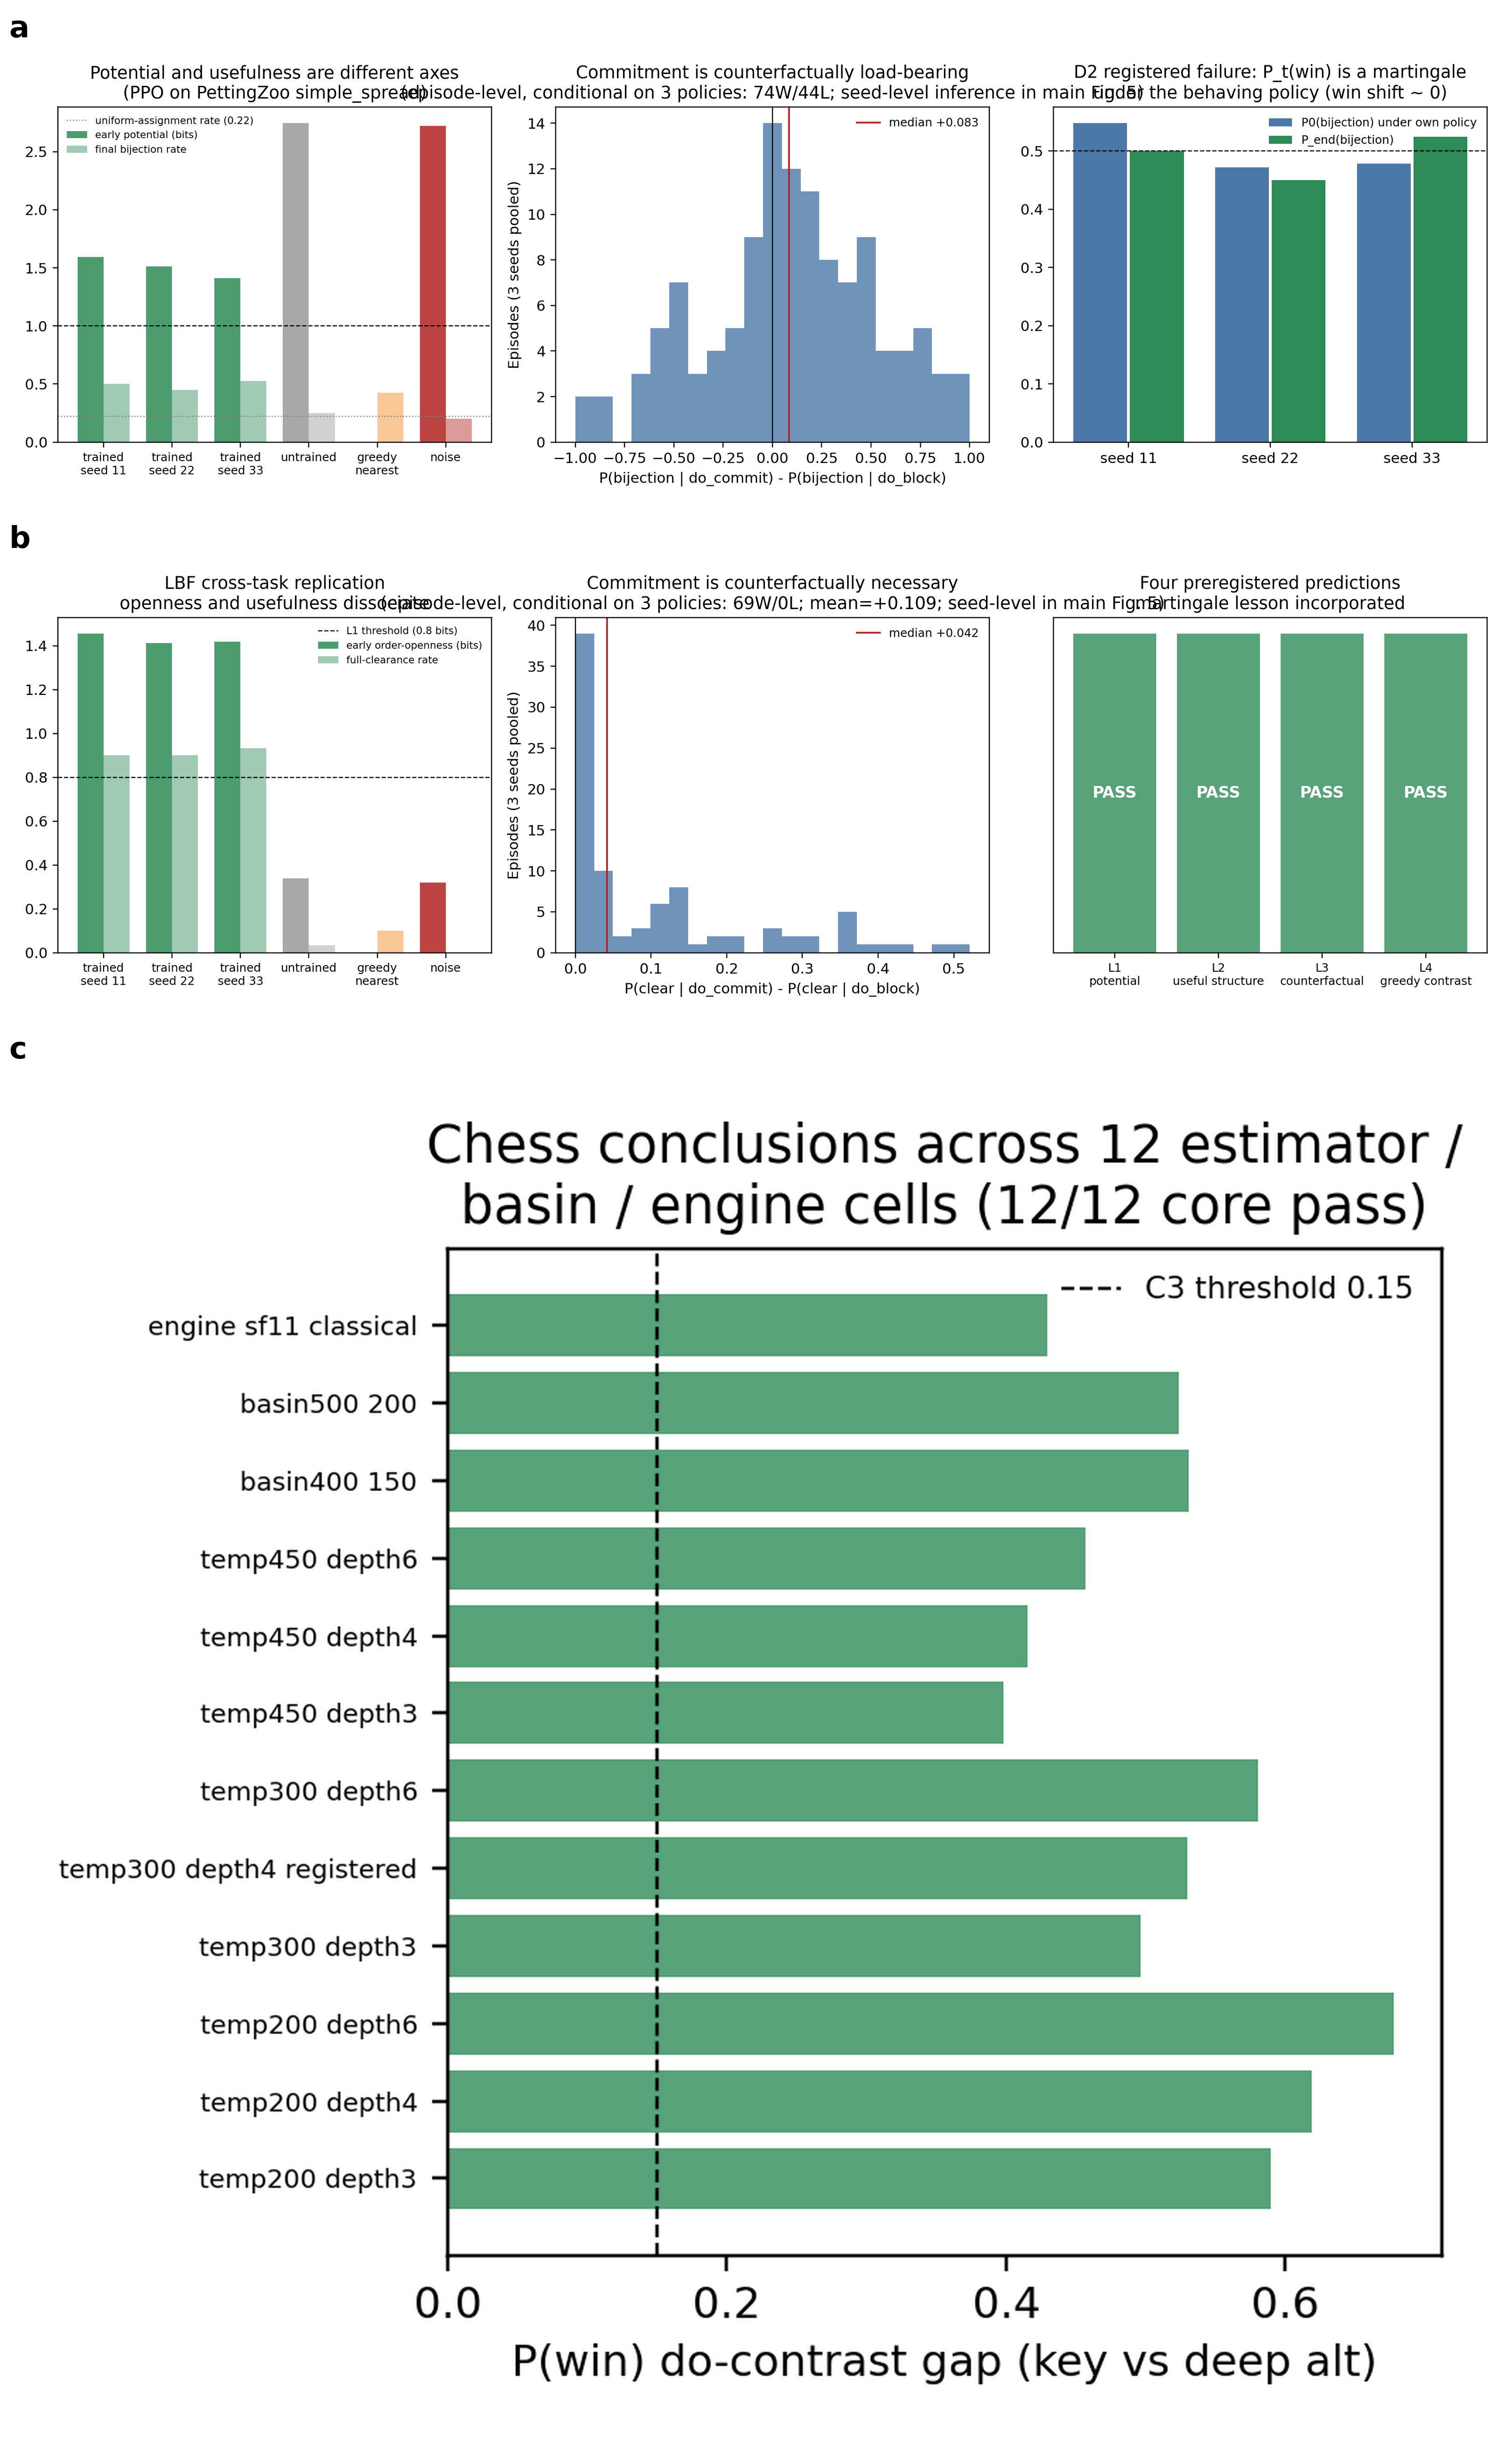
\includegraphics[width=\linewidth]{ed_fig12_episode_detail.png}
  \caption{\textbf{Episode-level MARL detail and the chess robustness
  grid.}
  \textbf{a}, simple\_spread (MAPPO): potential and usefulness are
  different axes---untrained openness does not qualify (left);
  episode-level do-contrast distribution, conditional on the three
  registered policies (middle); the registered D2 failure:
  $P_t(\text{win})$ is a martingale under the behaving policy (right).
  \textbf{b}, Level-Based Foraging cross-task replication: openness
  and usefulness dissociate again (left); blocking one agent's
  commitment destroys the joint outcome in 69/90 evaluation episodes,
  21 ties, no negative contrasts (middle); the four internally frozen
  predictions (right). Seed-level inference is in main
  Fig.~\ref{fig:marl}a.
  \textbf{c}, Chess: core do-contrast conclusions hold across 12
  estimator, basin and engine robustness cells.}
  \label{fig:ed-episode}
\end{figure}

\begin{figure}[p]
  \centering
  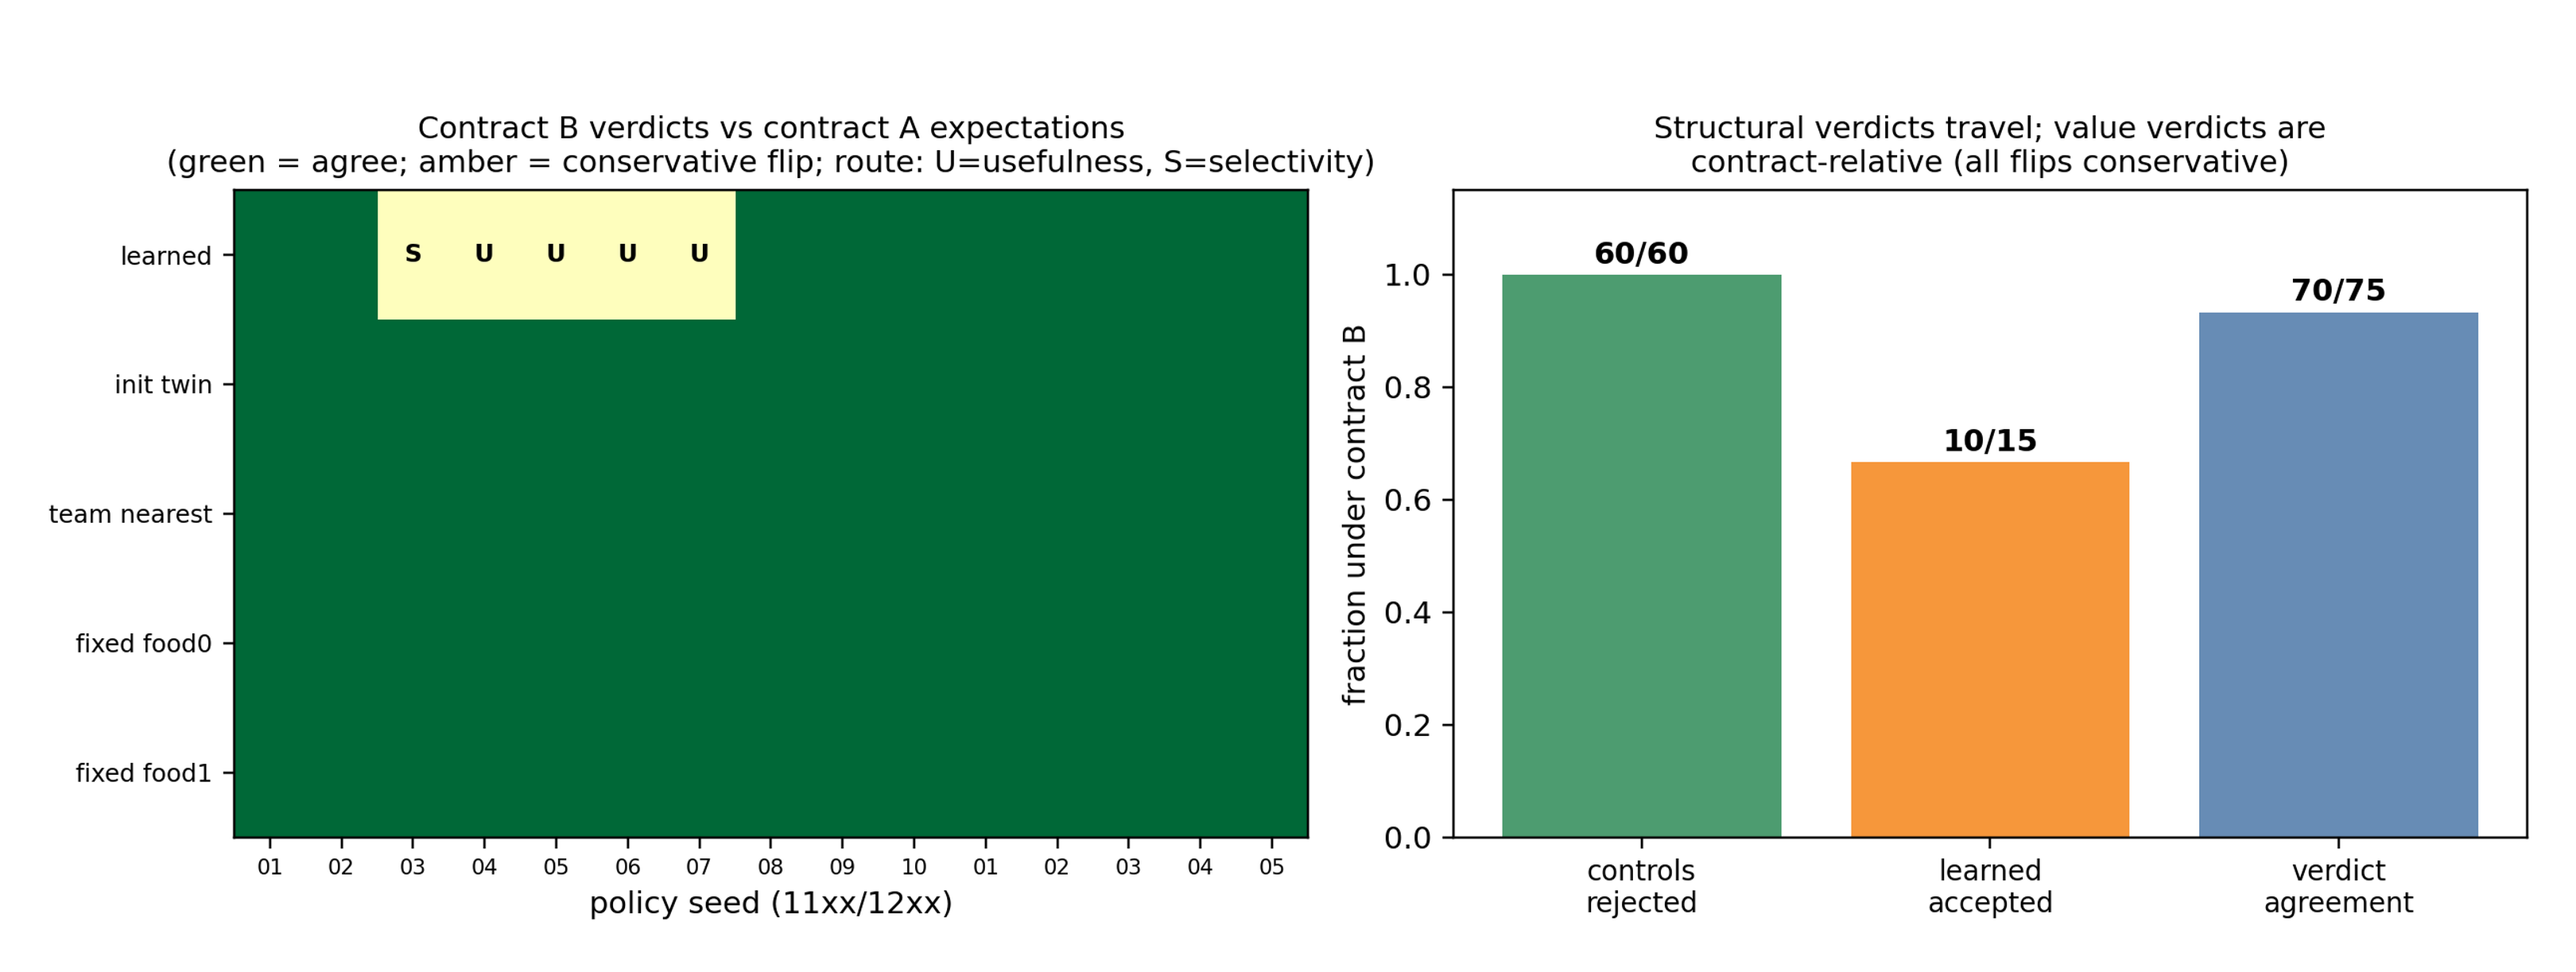
\includegraphics[width=0.95\linewidth]{ed_fig13_dual_observer.png}
  \caption{\textbf{Two plausible observer contracts on the Contextual
  LBF systems.}
  Contract B (declared before running) changes the horizon (15 to 12),
  the value function (discounted reward to undiscounted success) and
  the basin refinement (win/loss to completion speed) while still
  resolving the trigger identity. Left: verdict grid across all 75
  stored systems; every disagreement (amber) is a conservative
  rejection of a learned seed, routed through usefulness (U) in four
  cases and borderline selectivity (S) in one. Right: controls are
  rejected under both contracts (60/60); structural components agree
  on 14/15 learned seeds; the value component is contract-relative,
  as the layered definition declares.}
  \label{fig:ed-dualobs}
\end{figure}

\begin{figure}[p]
  \centering
  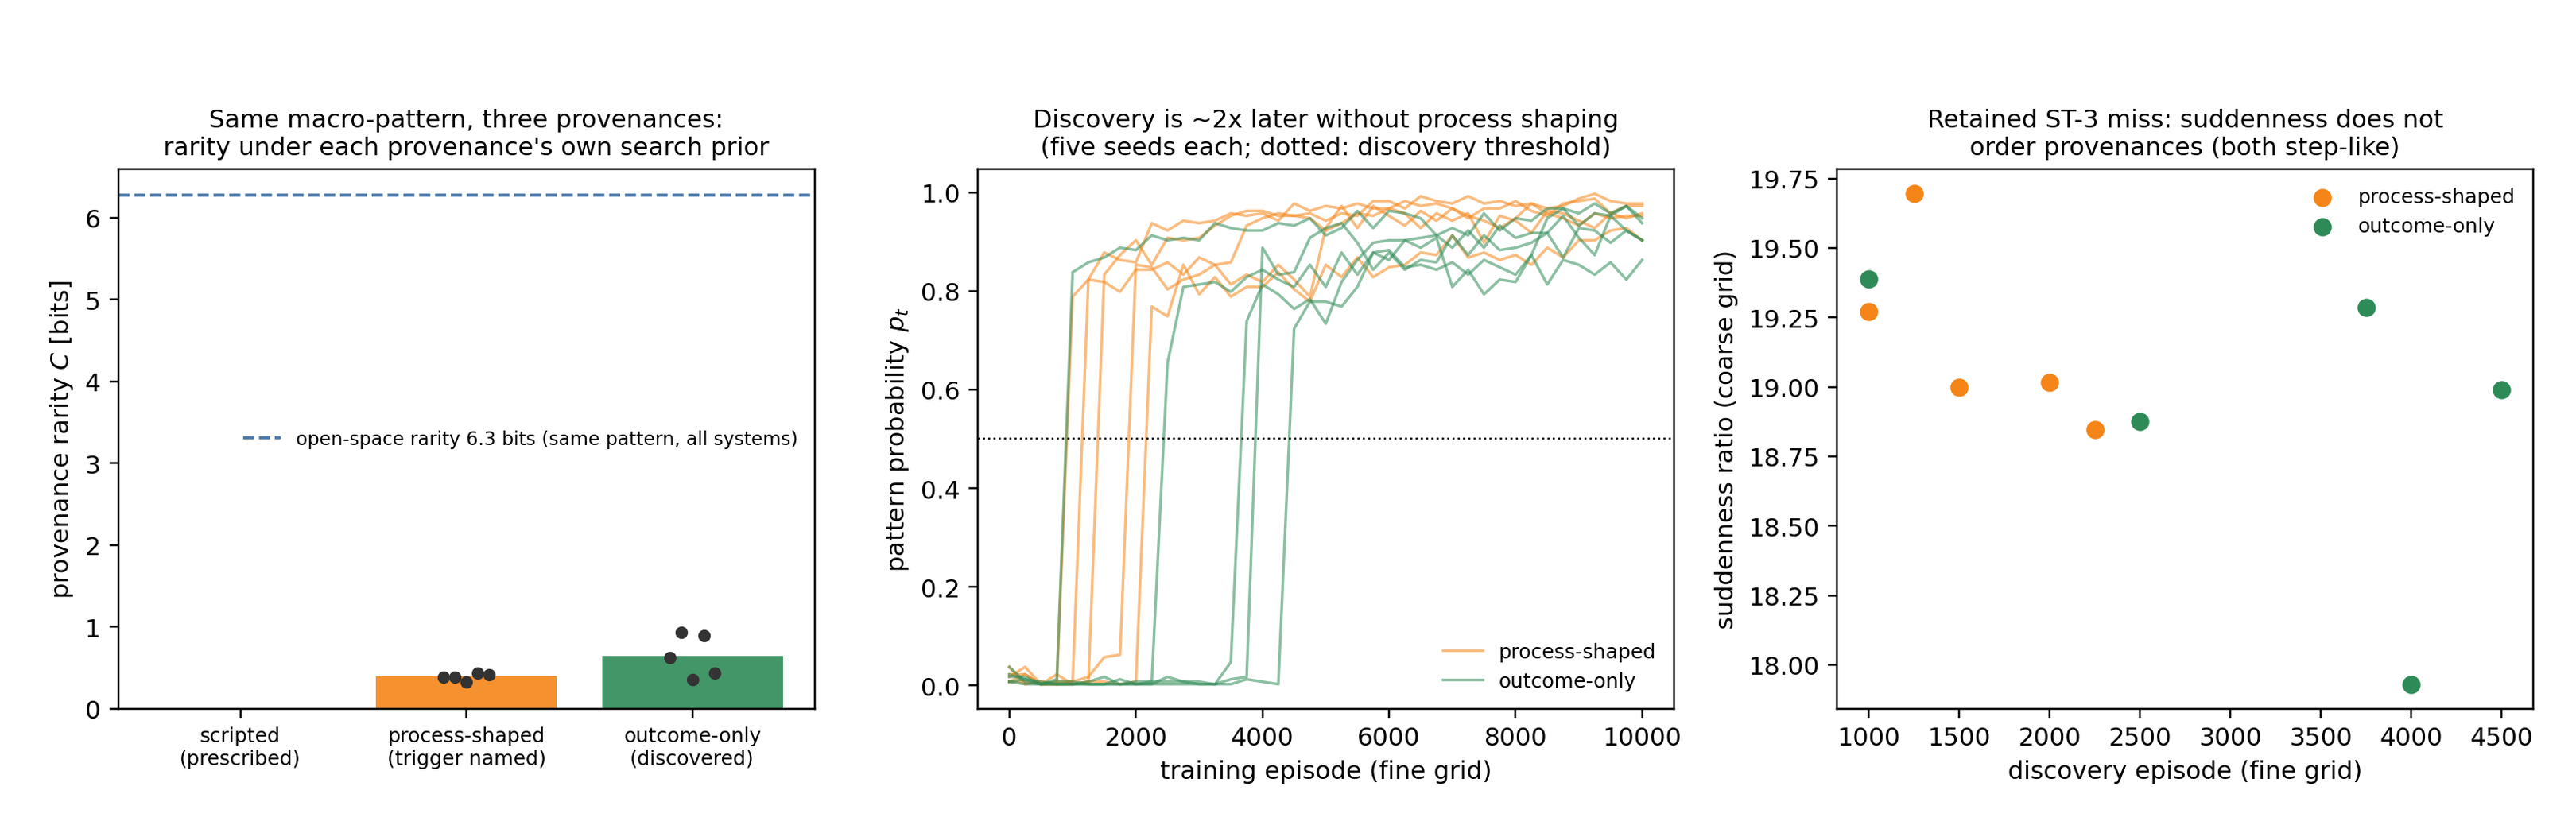
\includegraphics[width=\linewidth]{ed_fig14_strength_gradient.png}
  \caption{\textbf{Emergence strength as provenance rarity: one
  macro-pattern, three provenances.}
  Left: under the frozen open-space reference the sacrifice--rescue
  pattern is equally rare for every system ($6.3$ bits, dashed);
  under each provenance's own early search distribution the seed-mean
  rarity orders as the substrate predicts---scripted $0$ $<$
  process-shaped $0.39$ $<$ outcome-only $0.65$ bits (dots:
  individual seeds).
  Middle: fine-grid acquisition traces; the outcome-only provenance
  discovers the same pattern about twice as late as the
  process-shaped one, at matched final competence.
  Right: the retained ST-3 miss---collapse suddenness does not order
  the provenances, because both acquisitions are step-like at this
  grid; strength is carried by provenance rarity and discovery time,
  not burst shape.}
  \label{fig:ed-strength}
\end{figure}

\begin{figure}[p]
  \centering
  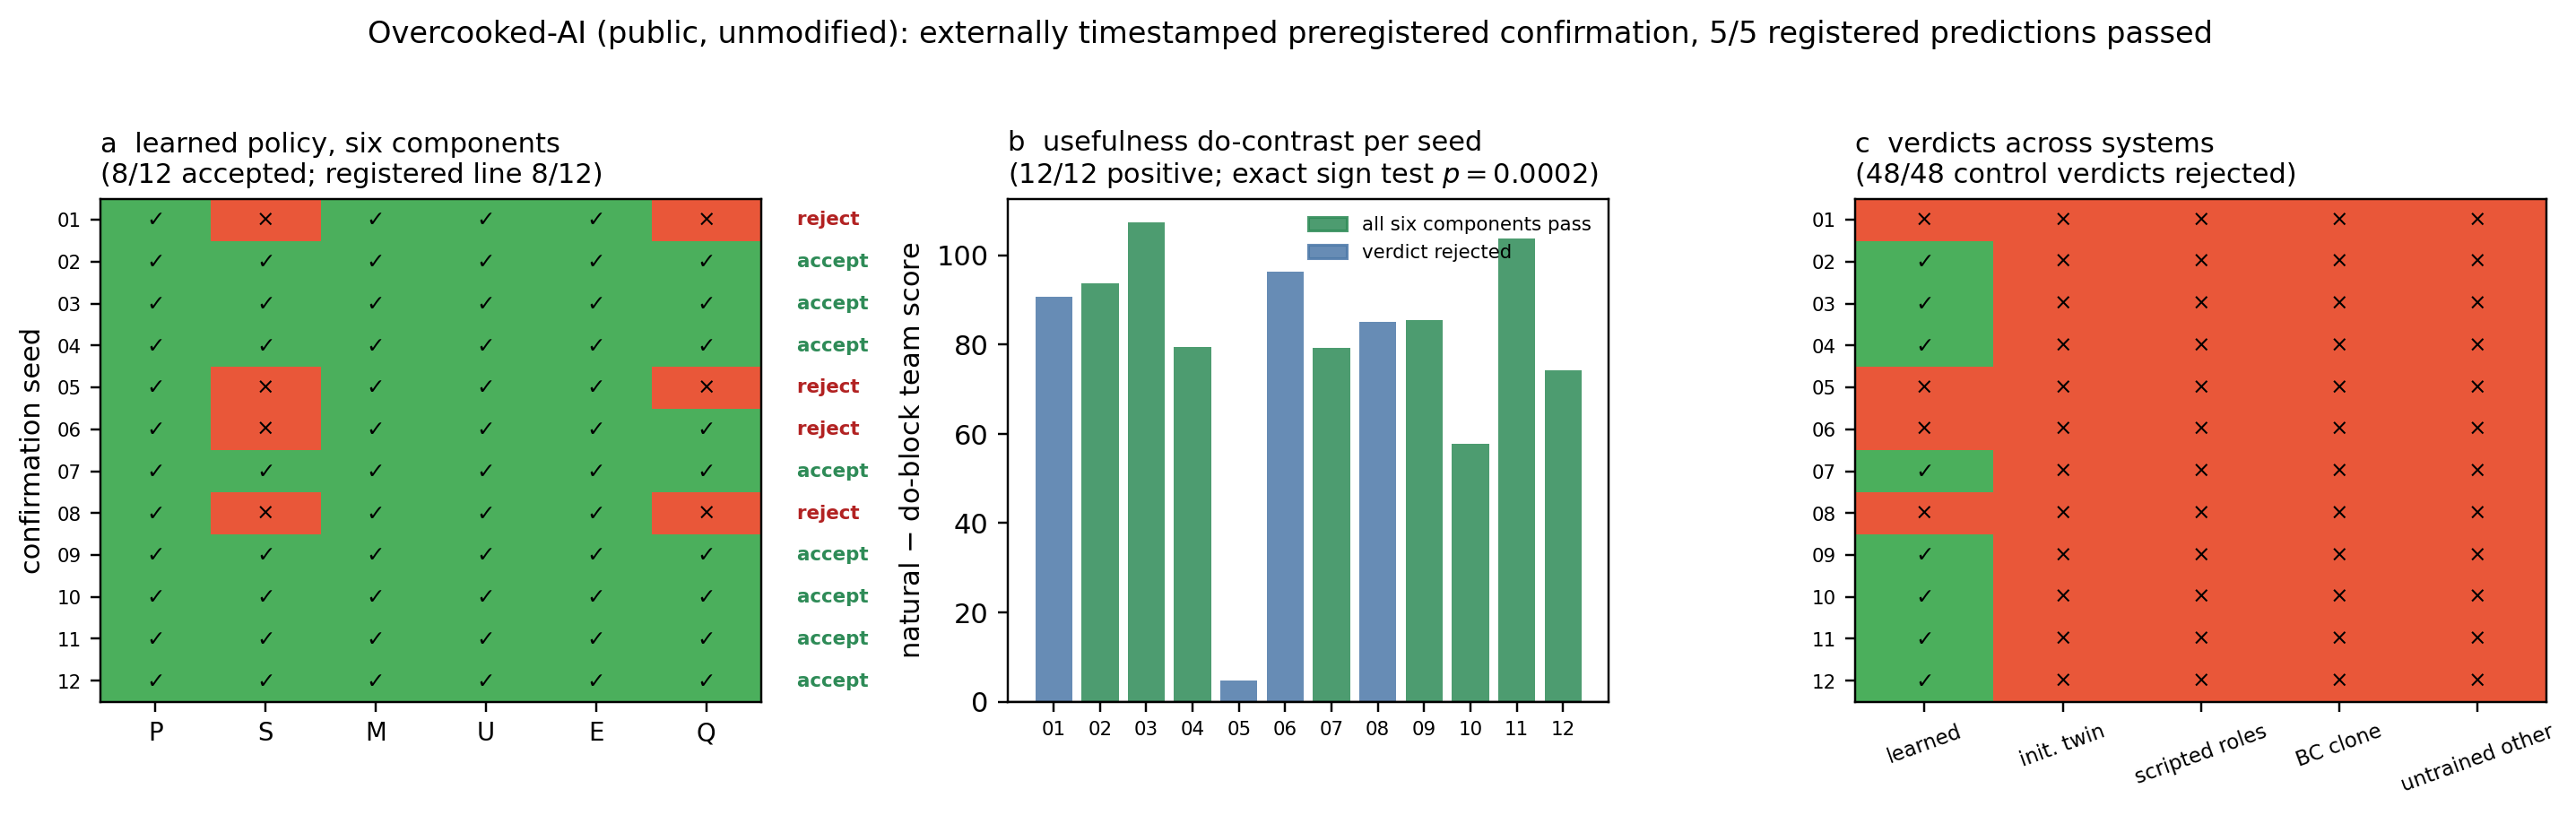
\includegraphics[width=\linewidth]{fig45_overcooked_confirmation.png}
  \caption{\textbf{Public third-party environment: externally
  timestamped, preregistered Overcooked-AI confirmation (all five
  registered predictions passed).}
  \textbf{a}, Per-seed six-component outcome for the learned self-play
  policy across the 12 confirmation seeds: 8/12 accepted, exactly the
  registered acceptance line; every rejection routes through
  conditional selectivity (with acquisition), the correct verdict for
  policies that pot indiscriminately in both layouts.
  \textbf{b}, The primary seed-level inference: the usefulness
  do-contrast (natural minus do-block team score) is positive on
  12/12 seeds (exact sign test $p=2\times10^{-4}$); colour marks
  full-certificate acceptance.
  \textbf{c}, All 48 control verdicts are rejections: scripted role
  pairs and their behavioural clones fail endogeneity and acquisition
  despite high competence; initialization twins and untrained pairs
  fail selectivity and usefulness. The protocol, thresholds and
  predictions were frozen with a public external timestamp before any
  confirmatory seed was launched (Methods).}
  \label{fig:ed-overcooked}
\end{figure}

\begin{figure}[p]
  \centering
  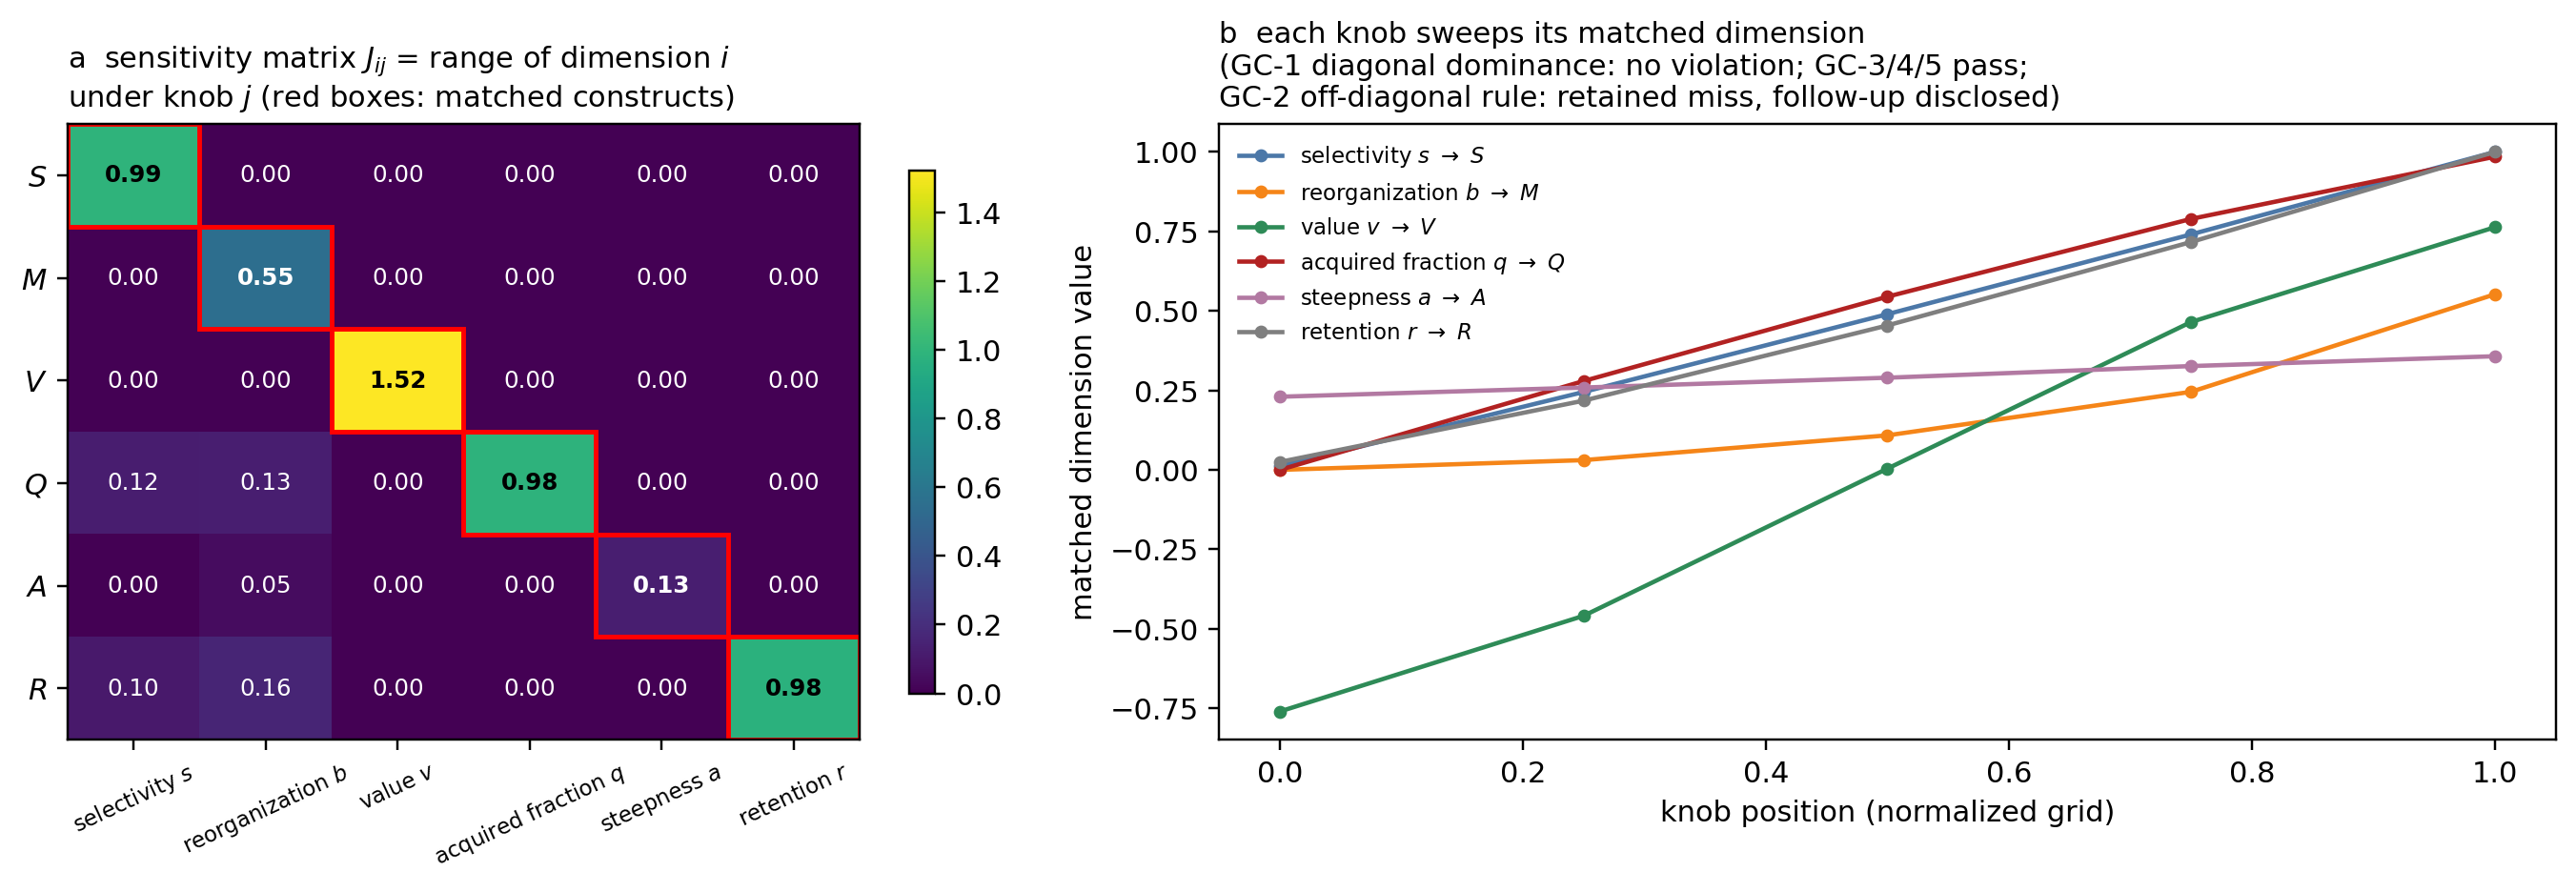
\includegraphics[width=\linewidth]{fig46_generator_calibration.png}
  \caption{\textbf{Six-knob ground-truth generator: the continuous
  record measures the constructs it names.}
  \textbf{a}, Sensitivity matrix: response range of each measured
  dimension (rows) as each generator knob (columns) sweeps its grid
  with all other knobs at reference values, averaged over measurement
  seeds; every measurement uses the same finite-sample estimator
  pipeline as the real systems. Red boxes mark the matched
  construct--knob pairs; the registered diagonal-dominance prediction
  passed with no violation.
  \textbf{b}, Matched sweeps: each knob moves its own dimension across
  its full range (selectivity $0.01\to1.00$, value $-0.76\to+0.76$,
  normalized acquisition $0.00\to0.99$, retention $0.03\to1.00$) while
  unmatched dimensions stay flat. Nullity (GC-3), value separability
  (GC-4) and provenance separability (GC-5) passed as registered; the
  off-diagonal suppression rule (GC-2) failed on two couplings and is
  retained---the frozen exemption list omitted the matched acquisition
  pair, and persistence responds to reorganization at $0.29$ of its
  diagonal because retention is retention \emph{of} structure.}
  \label{fig:ed-generator}
\end{figure}

\end{document}
